\documentclass{memoir}[11pt,oneside,a4paper,openany]
\PassOptionsToPackage{svgnames}{xcolor}
\usepackage{amsmath}
\usepackage{amssymb}
\usepackage{siunitx}
\usepackage{mhchem}
\usepackage{nth}
\usepackage{wrapfig}
\usepackage[hidelinks=true,colorlinks=false]{hyperref}
\usepackage{graphicx}
\usepackage{bm}
\usepackage{xspace}
\usepackage{booktabs}
\usepackage{tcolorbox}
\usepackage{braket}
\usepackage{subcaption}
\tcbuselibrary{skins,breakable}
\usetikzlibrary{shadings,shadows}

\newenvironment{myexampleblock}[1]{%
    \tcolorbox[beamer,%
    noparskip,breakable,
    colback=LightGreen,colframe=DarkGreen,%
    colbacklower=LimeGreen!75!LightGreen,%
    title=#1]}%
    {\endtcolorbox}

\newenvironment{myalertblock}[1]{%
    \tcolorbox[beamer,%
    noparskip,breakable,
    colback=LightCoral,colframe=DarkRed,%
    colbacklower=Tomato!75!LightCoral,%
    title=#1]}%
    {\endtcolorbox}

\newenvironment{myblock}[1]{%
    \tcolorbox[beamer,%
    noparskip,breakable,
    colback=LightBlue,colframe=DarkBlue,%
    colbacklower=DarkBlue!75!LightBlue,%
    title=#1]}%
    {\endtcolorbox}


\setlrmarginsandblock{2cm}{2cm}{*}
\setulmarginsandblock{2cm}{*}{1}
\checkandfixthelayout

\setlength{\parskip}{0.3cm}

\renewcommand{\thefootnote}{\fnsymbol{footnote}}

\newcommand{\wf}{\ensuremath{\bm{\Psi}}\xspace}
\newcommand{\dd}{\ensuremath{\mathrm{d}}}
\newcommand{\bv}{\ensuremath{\bm{v}}}
\newcommand{\bp}{\ensuremath{\bm{p}}}
\newcommand{\bj}{\ensuremath{\bm{J}}}
\newcommand{\bw}{\ensuremath{\bm{\omega}}}



\DeclareSIUnit{\mph}{mph}

\title{Introductory Quantum Mechanics - Handout}
\author{J. D. Pickering}

\begin{document}
\begin{titlingpage}
\maketitle
\end{titlingpage}
\tableofcontents
\chapter{Origins of Quantum Mechanics}

\section{The Breakdown of Classical Mechanics}
Since antiquity, humans have sought to develop rules that enable them to better understand the world around them. Since at least the time of Archimedes ($\sim$300BC) theories that allow the motion and behaviour of macroscopic objects to be described and predicted have been developed. During the Renaissance, scientists such as Galileo, Copernicus, and Kepler developed more and more descriptions of everyday observations - especially astronomical ones. By the end of the Renaissance, Sir Isaac Newton had laid the foundations of what is now known as `classical mechanics'. 

Classical mechanics describes the motion of macroscopic objects, i.e. things you can see. Newton's laws were (and still are) shown to be powerful formulations that beautifully describe many natural phenomena, and are still used today by engineers, doctors, and anyone who is working at the macroscopic scale. However, by the mid \nth{19} century, advancements in experimental techniques enabled scientists to make observations at a deeper level than had been previously possible. Many of the new observations that were made were found to be inconsistent with the classical descriptions of the previous two millenia. Two important observations, that illustrated the limitations of classical mechanics, are detailed below.

\subsection{Black-Body Radiation and the Rayleigh-Jeans Law}

\begin{wrapfigure}{r}{0.5\textwidth}
	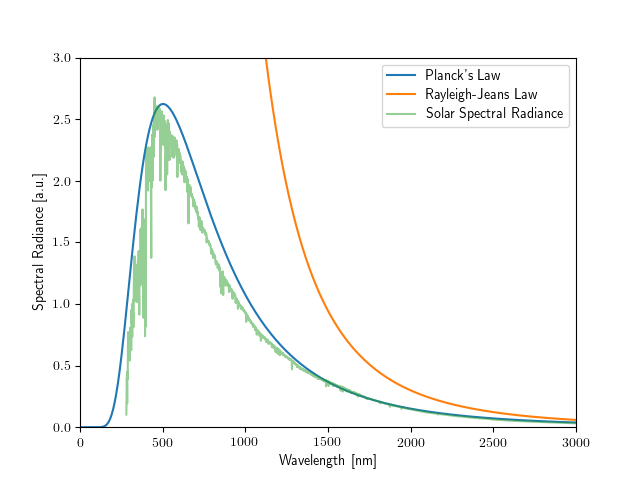
\includegraphics[width=\linewidth]{black_body.png}
	\caption{Black Body Radiation}\label{fig:black_body}
\end{wrapfigure}

Black-body radiation refers to the radiation that all objects emit when in equilibrium with their surroundings. Here when we refer to `radiation' we mean \emph{electromagnetic} radiation (i.e. radio waves/visible light/X rays), and not \emph{nuclear radiation}. A `black body' is an object which perfectly absorbs all radiation incident on it - and so appears black to human eyes. The frequency (or wavelength) of black-body radiation is strongly dependent on temperature. You will be familiar with this if you've ever seen metal heated in a flame or forge - at low temperatures the metal still appears grey; but as it gets hotter it starts to glow red, then orange, then yellow, and finally bright white. This is because the frequency of the black-body radiation increases as the temperature increases, and the wavelength of the emitted radiation goes from being infrared (invisible), to visible. 

Attempts to describe black-body radiation classically were made by Lord Rayleigh and James Jeans, who developed the \emph{Rayleigh-Jeans} Law given in~\autoref{eq:rayleigh_jeans}. This law relates the spectral radiance\footnote{Spectral radiance is literally what it sounds like, it's a measure of how radiant/bright something is at different wavelengths} $B_\lambda$ at a wavelength $\lambda$ to the temperature of the body, $T$.

\begin{equation}\label{eq:rayleigh_jeans}
	\centering
	B_\lambda(\lambda,T) = \frac{2ck_B T}{\lambda^4}
\end{equation}

The sun is (to a reasonable approximation) a black-body (but it appears orange because it's so hot), and the spectral radiance of the sun is shown in green on~\autoref{fig:black_body}. The temperature of the sun is \SI{5777}{\kelvin}, and the Rayleigh-Jeans spectral radiance of a black-body at \SI{5777}{\kelvin} is shown in orange on~\autoref{fig:black_body}. Compared to the true spectrum of the sun, it is clear that at long wavelengths, the Rayleigh-Jeans spectrum matches well. However, it fails spectactularly at short wavelengths - infact the Rayleigh-Jeans law would predict that at room temperature, every object is emitting bright ultraviolet light, an obviously unphysical situation known as the \textbf{ultraviolet catastrophe!}

\begin{equation}\label{eq:plancks_law}
	\centering
	B_\lambda(\lambda, T) = \frac{2hc^2}{\lambda^5} \frac{1}{\exp{\frac{hc}{\lambda k_B T}}-1}
\end{equation}

The situation was resolved by Max Planck who derived \emph{Planck's Law} (\autoref{eq:plancks_law}), by assuming that energy could only be emitted in discrete, fixed amounts. It is clear from\autoref{fig:black_body} that the spectral radiance predicted by Planck's Law (blue) is a much better fit to the experimental data than the Rayleigh-Jeans law. This was among the first evidence for the \textbf{quantisation of energy} - the idea that energy only exists in discrete `packets'. In the case of EM radiation (light), these packets are called \emph{photons} - and can be thought of as particles with energy $E=\hbar\omega$, where $\omega$ is the frequency of the light. Classical physics had always described light as a wave, but Planck's law started to suggest that this picture was incomplete. Albert Einstein went on to provide more evidence of this incomplete classical picture.   

\subsection{The Photoelectric Effect}
\begin{wrapfigure}{r}{0.5\textwidth}
	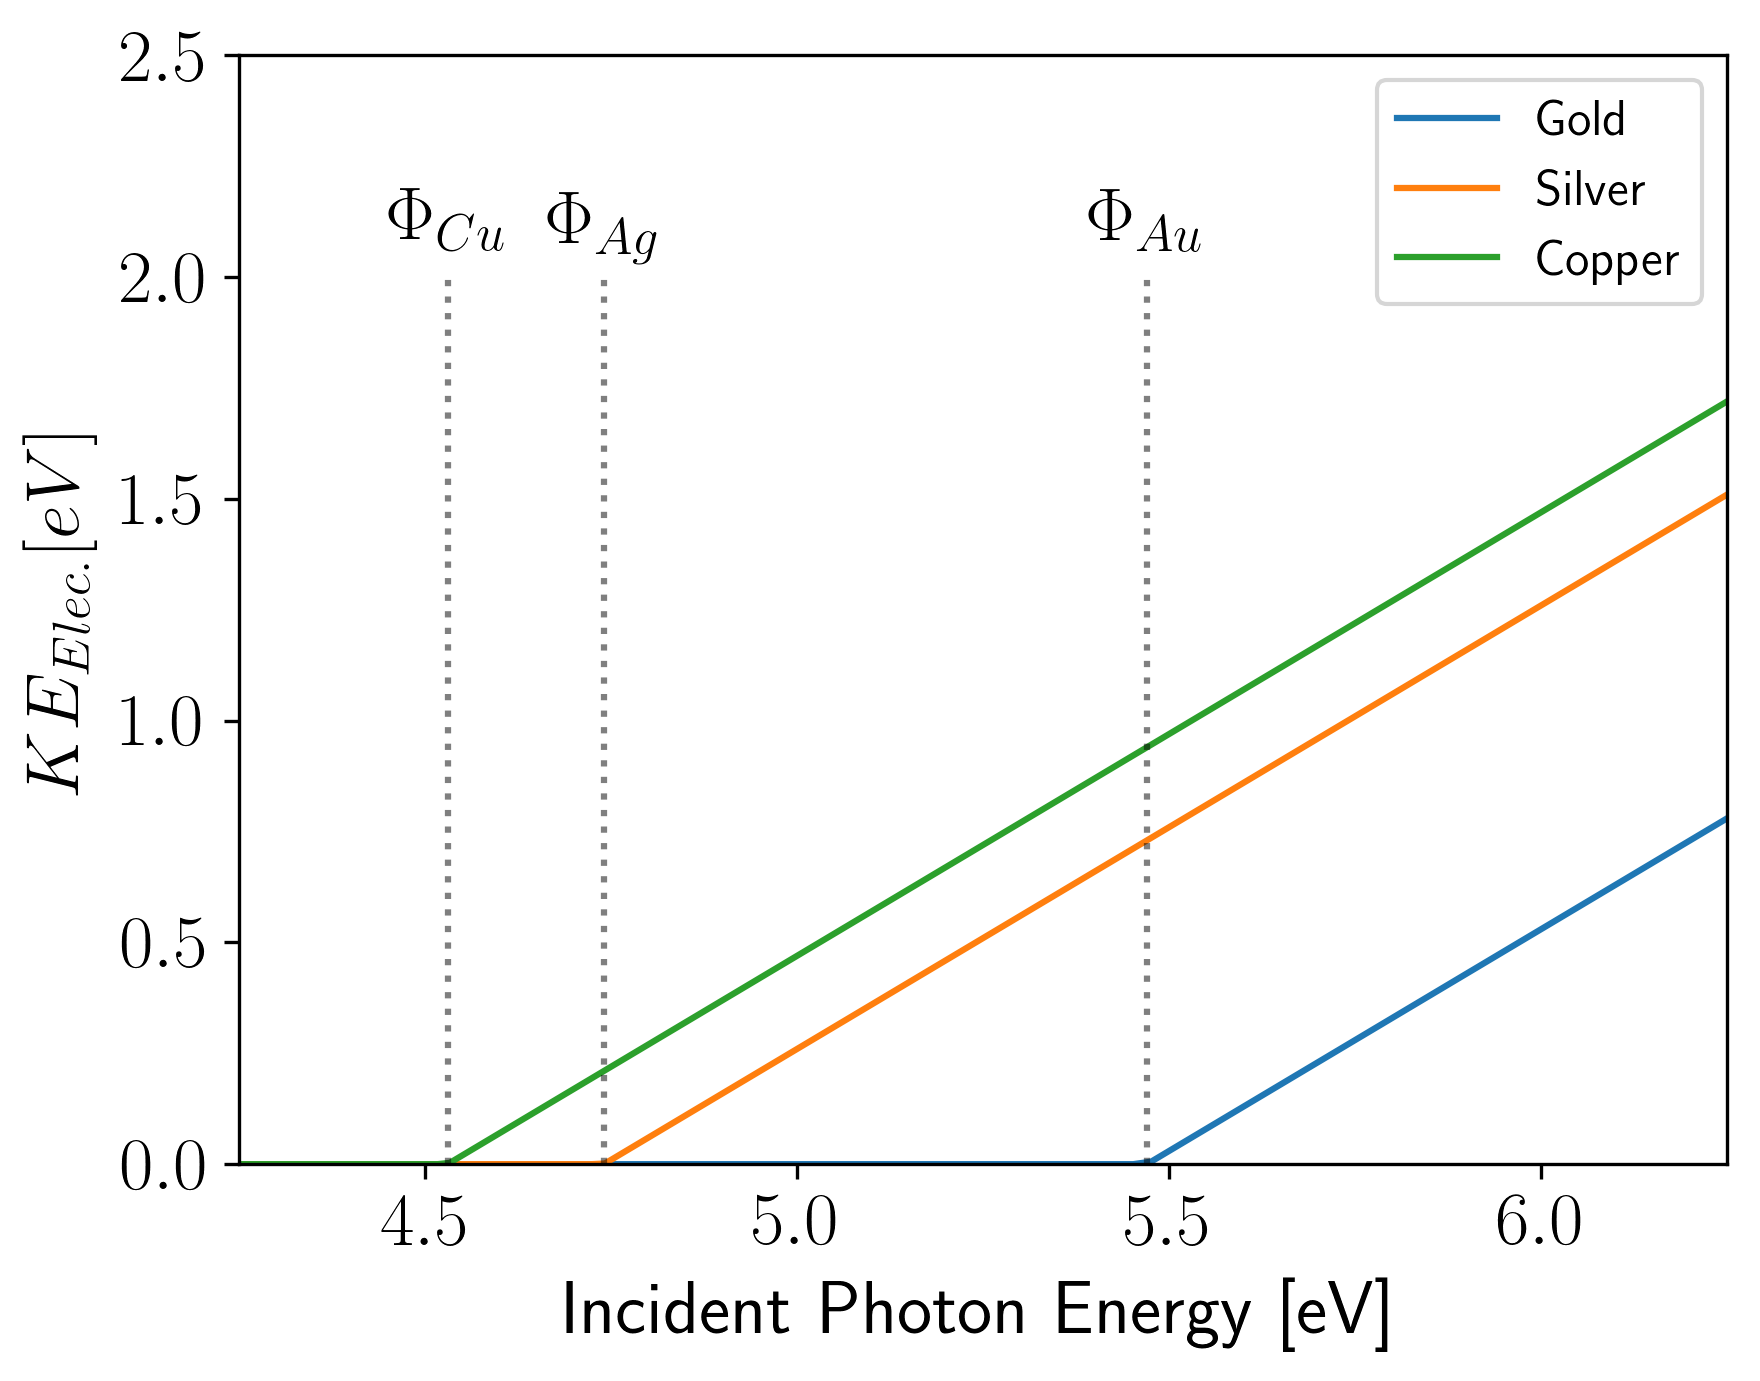
\includegraphics[width=\linewidth]{photoelectric.png}
	\caption{Photoelectric Effect}\label{fig:photoelectric}
\end{wrapfigure}
Further evidence for the impending breakdown of classical mechanics came from Albert Einstein's description of the \emph{photoelectric effect}. The photoelectric effect is the observation that electrons can be emitted by metals when light is shined on them. Classically it was expected that brighter light would result in higher energy electrons being emitted. Yet it was found that the energy of the ejected electrons did not depend on the intensity (brightness) of the incident light, but only on the colour (frequency) of the light. Furthermore, materials didn't ejecting any electrons until a certain \emph{threshold frequency} (normally in the ultraviolet range) was exceeded - it wouldn't matter how bright the light was that you shone, no electrons would be emitted if it wasn't the right colour! The kinetic energy of the ejected electron also increased linearly as the frequency of the light was increased (increasing frequency means that the colour moves from red to blue, and into the UV). This is illustrated in~\autoref{fig:photoelectric}.

Einstein showed that the kinetic energy of an ejected electron was given by"\autoref{eq:photoelectric}, where $\Phi$ is an intrinsic property of the metal known as the \emph{work function}, and $\hbar\omega$ is the energy of the incident photon ($\omega$ is the frequency of the light). Central to his model was the idea that the light behaved as a `packet' of energy $\hbar\omega$ - this `packet' is a photon. One can imagine the process as a collision between a photon and the metal that results in the photon knocking off an electron. If the photon only just has enough energy to overcome the work function, then the energy of an ejected electron is very low. If the photon has an energy which is much greater than the work function, then the excess energy becomes the kinetic energy of the ejected electron, $KE_{elec.}$. 
\begin{equation}\label{eq:photoelectric}
	KE_{elec.} = \hbar\omega - \Phi
\end{equation}
The equation above is plotted in \autoref{fig:photoelectric} for three different metals - it is clear that the energy of the incident photon has to pass some threshold before a photoelectron is emitted. This plot also provides a direct way to measure Planck's constant, $h$ - can you see how?


\subsection{Wave-Particle Duality}
Einstein's description of the photoelectric effect provided clear evidence for the particle (photon) nature of light (which was classically thought of, and modelled as, a wave). The wave description of light explains many phenomena very well, such as diffraction and interference; but we have seen that other phenomena (such as the photoelectric effect), are better modelled using the particle (photon) description. In reality, there is nothing contradictory about this - sometimes the wave picture is more useful and sometimes the particle picture is more useful - both are valid! This concept is referred to as \emph{Wave-Particle Duality}, and is a \textbf{central} concept in quantum mechanics.

You should be familiar with the concept of a \textbf{de Broglie Wavelength} from \nth{1} year physical chemistry. To briefly recap, de Broglie postulated that any particle (e.g. a photon, an electron, an atom, or a potato) travelling with linear momentum $p$\footnote{Remember $p = mv$.}, also has a wavelength $\lambda_{dB}$ given by~\autoref{eq:de_broglie}.
\begin{equation}\label{eq:de_broglie}
	\lambda_{dB} = \frac{h}{p}
\end{equation}
In the case of something like a potato, the de Broglie wavelength is so tiny (because the momentum is so huge) that it is impossible to detect the wave nature of the particle. However, for things like electrons (tiny mass and therefore tiny momentum), the wave-like nature can be observed - for instance in the \emph{Davisson-Gerner} experiment, where electrons were diffracted from a crystal lattice, much like light can be diffracted through a grating.

This idea of \emph{Wave-Particle Duality} is like a stake driven into the heart of classical physics, where waves and particles were treated as entirely separate entities. This picture was clearly inconsistent with empirical observations, so had to be amended. To quote Albert Einstein:
\begin{quote}
	\textit{``We have two contradictory pictures of reality; separately neither of them fully explains the phenomena of light, but together they do''.}
\end{quote}
A consequence of Wave-Particle Duality is that rather than thinking of particles as travelling along well-defined trajectories, they should instead be thought of as being spread out in space like a wave. The mathematical formulation that describes this trajectory is called the \textbf{Wavefunction}.

\section{Wavefunctions and Mathematical Tools}
The concept of a \textbf{wavefunction} is key concept going forward - however it comes with some mathematical baggage if a full understanding is desired! 

\subsection{Wavefunctions and the Schr{\"o}dinger Equation}
The wavefunction (henceforth referred to as \wf for brevity) contains \emph{all the dynamical information about the system that it describes}. `Dynamical information' means all the information about where the system is, what energy it has, and how it's changing. That is to say, that if we want to calculate any physical property of a system, all we need to do is find the wavefunction of that system! This sounds very powerful (and it is!), but in reality it can be tricky/impossible to find wavefunctions that will describe complex systems (such as anything macroscopic, or even large molecules). An obvious question is then - how is a wavefunction calculated?

The equation that allows the wavefunction of any system to be calculated is named after Erwin Schr{\"o}dinger - \textbf{The Schr{\"o}dinger Equation} - and probably ranks in the top 3 (if not at the top) of any `Most Important Equations in the World' list. Strictly, there are two variants, the \emph{Time-Dependent Schr{\"o}dinger Equation} (TDSE), and the \emph{Time-Independent Schr{\"o}dinger Equation} (TISE). The TDSE is the most general form, but we will solely focus on the TISE - as this is the most relevant for us as chemists (we tend to be interested in calculating things on static molecules - at least initially). The TISE is given in~\autoref{eq:tise}, drum roll please...

\begin{equation}\label{eq:tise}
	\hat{H}\wf = E\wf
\end{equation}

This looks remarkably simple! Unpacking it, it tells us that the \textbf{Hamiltonian Operator} $\hat{H}$ of a system \emph{operating} on the wavefunction \wf, produces the total energy of the system $E$, multiplied by the original \wf. It also tells us that we can find a wavefunction for any system by solving this equation - solving the Schr{\"o}dinger Equation directly is beyond the scope of this course, but the solutions will be presented in due course. What is actually happening here (including what an \textbf{operator} actually is) will be explained more thoroughly in the following sections. 

\subsection{The Born Interpretation and Normalisation}
Before embarking on a quest to solve the Schr{\"o}dinger Equation, it is worth exploring the properties of wavefunctions in more detail. We said in the previous section that the wavefunction contains \textbf{all dynamical information about the system that it describes}. We will see how we can extract different kinds of information in the following sections, but first it is useful to focus on the simplest information - the location of the particle in the system. 

Max Born developed a law which is known as `Born's Law', or `The Born Interpretation'\footnote{Not to be confused with any of Matt Damon's action films.}. Simply, this law states that the probability density of finding a particle at a certain position in a system is proportional to the square modulus of the wavefunction at that position. Mathematically:
\begin{equation}
	P(X=x) \propto \lvert \wf(x) \rvert ^2 \mathrm{d}x 
\end{equation}
Where $P(X=x)$ is the probability that the position ($X$) of the particle is at $x$ (in a region of width $\mathrm{d}x$). This probability is proportional to the square modulus ($\lvert \wf \rvert ^2 = \wf \wf^*$, if $\wf$ is complex) of the wavefunction multiplied by the width of the region. This looks like a lot of maths - but it's actually quite simple. It's saying that the probability of finding the particle at some point between $x$ and $x+\mathrm{d}x$ is proportional to square modulus of \wf, multiplied by $\mathrm{d}x$. If we made $\mathrm{d}x$ massive, then the probability would be massive too - which makes sense as the probability of finding the particle in a big area is bigger than the probability of finding it in a small area! 

We can extend this now, and ask what the probability of finding the particle between two limits is, say between two locations $a$ and $b$? All we need to do is to sum the probability density over the area bounded by $a$ and $b$ - which can be easily done via integration:
\begin{equation}
	P(a\leq x \leq b) = \int_a^b \lvert \wf(x) \rvert ^2 \mathrm{d}x
\end{equation}

A useful question to ask now, is what is the probability that we find the particle in \emph{any location in space}? Obviously, we have to find the particle \textbf{somewhere}! We can write this mathematically by saying that the probability of finding the particle anywhere in space has to be 1:
\begin{equation}\label{eq:normalisation}
	P(\text{anywhere}) = \int_{-\infty}^{\infty} \lvert \wf(x) \rvert ^2 \mathrm{d}x = 1
\end{equation}

This puts some limitations on what an acceptable wavefunction can be - it has to satisfy the equation above, which means it cannot be infinite anywhere. If it were infinite anywhere, then the probability of the particle being at that location would be infinite, which is clearly unphysical! By the same argument, it cannot be zero everywhere - the particle needs to be somewhere! Additionally, the wavefunction has to be \emph{single-valued}, meaning that there can only be one value of $\wf(x)$ at each value of $x$. If this were not the case, then the probability of a particle being at a position $x$ would have multiple values - which is clearly nonsensical\footnote{Imagine if I told you that the probability of there being a cup of tea on my desk was simultaneously 40\% likely and 90\% likely.}! We will return to these constraints (and add more) later.

Now we come to the concept of \textbf{normalisation}. Normalisation is the process of making wavefunctions satisfy~\autoref{eq:normalisation}. It is a mathematical feature of the Schr{\"o}dinger Equation that if \wf is a solution, then $N \times \wf$, where $N$ is a constant, is also a solution. This is very convenient, as it means we can actually make more or less any wavefunction satisfy \autoref{eq:normalisation}, as:
\begin{equation}
	P(\text{anywhere}) = \int_{-\infty}^{\infty} \lvert N\wf(x) \rvert ^2 \mathrm{d}x = N^2 \int_{-\infty}^{\infty} \lvert \wf(x) \rvert ^2 \mathrm{d}x = 1
\end{equation}
Where we call $N$ the \emph{normalisation constant}, which we can pull out of the front of the integral as it's just a constant. We just have to pick the value of $N$ such that the above equation is satisifed, i.e:
\begin{equation}
	N = \frac{1}{\sqrt{\int_{-\infty}^{\infty} \lvert \wf(x) \rvert ^2 \mathrm{d}x}}
\end{equation}
We will see some examples of this, and normalise some of our own wavefunctions, in due course.

\subsection{Hamiltonians, Operators, and Observables}
We previously referred to the \textbf{Hamiltonian Operator}, $\hat{H}$, of a system. The small `hat' on top of the $H$ denotes that this is an \textbf{operator}. An operator is simply something that tells you to carry out a mathematical operation on whatever follows it. For example, I could define an operator $\hat{O} = 2\times$, which simply doubles whatever it operates on - i.e. $\hat{O}3 = 2\times 3 = 6$. That's all operators are - just mathematical instruction sheets. 

The \textbf{Hamiltonian Operator} is slightly more complicated - it's operation is that it calculates the \emph{total energy} of the system it operates on. You can think of it as just an instruction that you give to the wavefunction of a system to tell it to give you the total energy of the system back to you. The specific form of the Hamiltonian Operator depends on the system we're applying it to - for the sake of argument let's imagine that we are interested in a single particle of mass $m$ moving in one dimension. 

From basic physics we know that the total energy of any particle, $E_{\text{Total}} = E_{\text{Kinetic}} + E_{\text{Potential}}$, i.e. the total energy is the sum of the kinetic and potential energies. When we write our Hamiltonian, we therefore need to have a part of it that calculates the kinetic energy and a part of it that calculates the potential energy. The mathematics of how these are derived is beyond the scope of this section, but is in~\autoref{app:operator_construction} for interested readers. The full Hamiltonian for a particle of mass $m$ moving in one dimension along $x$, consisting of both kinetic ($\hat{H}_{\text{Kin.}}$) and potential ($\hat{H}_{\text{Pot.}}$) energy terms, is given in~\autoref{eq:hamiltonian_1d}. 

\begin{equation}\label{eq:hamiltonian_1d}
	\hat{H} = \hat{H}_{\text{Kin.}} + \hat{H}_{\text{Pot.}} = -\frac{\hbar^2}{2m} \frac{\mathrm{d}^2}{\mathrm{d}x^2} + V(x)
\end{equation}

The first term of~\autoref{eq:hamiltonian_1d} is the operator that gives the kinetic energy of the particle, and the second term is the operator that gives the potential energy. So, mathematically what we do is take the second derivative of \wf, multiplied by $-\frac{\hbar^2}{2m}$, and then add on $V(x) \times \wf$. If we do all this correctly, then we extract the total energy of our system, as shown in~\autoref{eq:tise_1d}.

\begin{equation}\label{eq:tise_1d}
	\hat{H}\wf = \hat{H}_{\text{Kin.}} + \hat{H}_{\text{Pot.}} = -\frac{\hbar^2}{2m} \frac{\mathrm{d}^2\wf}{\mathrm{d}x^2} + V(x)\wf = (E_{\text{Kin.}}+E_{\text{Pot.}})\wf = E_{\text{Total}} \wf
\end{equation}

So we can see that \textbf{operating on \wf with the Hamiltonian operator produces the total energy of the system.} Here the total energy is referred to as an \textbf{observable} - i.e. something we can physically measure. Operators and observables correspond in this way generally - we can define operators that will produce any physical observable when applied to a wavefunction. For example, we could define an operator for linear momentum, $\hat{p}$, which, when used on a wavefunction of a system, will return the linear momentum $p$ (an observable) of that system. We will see some specific examples of this in later sections, but for now just remember that operators and observables correspond in this way.  

A final point to note here relates to the acceptability of wavefunctions, that we started to discuss in the previous section. We already showed that a wavefunction has to be \emph{single valued}, and that a wavefunction \emph{cannot be infinite anywhere or zero everywhere}. The second derivative in \autoref{eq:hamiltonian_1d} adds another constraint - namely that we have to be able to compute the second derivative of the wavefunction. Specifically, this means that the wavefunction needs to be continuous (no sharp kinks or steps), and that the first derivative of the wavefunction also has to be continuous. 

We now have all the constraints that are placed on wavefunctions if they are to be acceptable. These constraints are quite strict, and actually it turns out that it's not normally possible to find acceptable wavefunctions for arbitrary values of $E$. Generally, you can \textbf{only find acceptable wavefunctions for specific energies of the system}. This, then, is where quantisation arises, as a particle can only have certain, discrete, energies if it is to have an acceptable wavefunction. I think this is quite a beautiful result!

\subsection{Eigenvalues and Eigenfunctions}
If you remember back to A level maths, you might see that the Schr{\"o}dinger equation written in \autoref{eq:tise} is an example of an \textbf{eigenvalue equation}. To refresh memories, we could write a general eigenvalue equation as:
\begin{equation}
	\text{(Operator)(Eigenfunction)} = \text{(Eigenvalue)}\times\text{(Eigenfunction)}
\end{equation}
The \textbf{eigenvalue} is always a \textbf{scalar} - that is a \textbf{constant}. The \textbf{eigenfunction}, in contrast, is a function, or a \textbf{vector}. So we can see that the way this equation works is that when you \textbf{operate} on an \textbf{eigenfunction}, what you get back is just a \textbf{constant} (the eigenvalue), multiplied by your original \textbf{eigenfunction}.Note that in some texts you will see the eigenfunction called an \textbf{eigenvector} - it's the same thing.  

We can illustrate how this works with a simple example. Taking a wavefunction $\phi(x) = \sin(ax)$, where $a$ is a constant, and taking our Hamiltonian to be $\hat{H} = \frac{\mathrm{d}^2}{\mathrm{d}x^2}$ (ignoring the usual prefactor and potential energy for simplicity). We can see that:
\begin{equation}
	\hat{H}\phi(x) = \frac{\mathrm{d}^2\phi(x)}{\mathrm{d}x^2} = \frac{\mathrm{d}^2}{\mathrm{d}x^2} \sin(ax) = -a^2 \sin(ax) = -a^2\phi(x)
\end{equation}
So we can now say that $\sin(ax)$ is an eigenfunction of $\hat{H}$, with the eigenvalue $-a^2$. Simple! Can you show that $\sin(ax)$ is \textbf{not} an eigenfunction of $\hat{O} = \frac{\mathrm{d}}{\mathrm{d}x}$? 

If we apply this to the example in the previous section, we could say that when a \textbf{wavefunction} is an eigenfunction of our \textbf{Hamiltonian}, then the resulting eigenvalue corresponds to the \textbf{total energy} of the system described by the wavefunction. 

We can also look at this as a place where quantisation comes from, as there aren't actually that many acceptable solutions of the Schr{\"o}dinger Equation (as we stated in the previous section). In general it's only possible to find eigenfunctions and eigenvectors that satisfy the Schr{\"o}dinger equation for \textbf{specific, discrete energies} - hence quantisation. We will see some more concrete examples of this later on though. 

\subsection{Expectation Values of Operators}
A useful thing to be able to calculate is the \textbf{expectation value} of an operator. The expectation value of a measurement is the \emph{most probable} outcome of it. If we calculate the expectation value of an operator, then what we're actually finding is the \emph{most probable value of the corresponding observable} - as we saw that operators and observables correspond in the previous sections.

The expression for the expectation value $\langle O \rangle$ of the observable $O$, is given by:
\begin{equation}
	\langle O \rangle = \int \wf^* \hat{O} \wf \,\mathrm{d}\tau
\end{equation}
Where $\hat{O}$ is the operator corresponding to observable $O$, and $\mathrm{d}\tau$ denotes an integral over \emph{all space}. This equation is only valid for \emph{normalised wavefunctions}, but is very powerful. It allows us to calculate the average value of any physical quantity associated with a system, provided we have a good wavefunction and an operator corresponding to the quantity! For example, we can calculate the average value of the energy, $\langle E \rangle$, as:
\begin{equation}
	\langle E \rangle = \int \wf^* \hat{H} \wf \,\mathrm{d}\tau
\end{equation}

You'll probably come across this result again in the course of your degree in the context of \emph{the variational theorem} - something you'll do in more advanced quantum mechanics and computational chemistry. For now, it's sufficient just to know that it exists. However, after the previous few sections, some of you are probably asking: what operators exist and how can we determine them?

Construction of operators is quite simple but is beyond the scope of this document (see~\autoref{app:operator_construction}). But see the table below where some common physical observables and their corresponding operators - we won't go into detail, but just for your own interest. We will meet some of these later on in this course. 
\begin{table}[h!]
	\centering
\begin{tabular}{@{}ll@{}}
\toprule
Observable & Corresponding Operator \\ \midrule
Position (1D along x) & $\hat{x} = x$ \\
Linear Momentum (along x) & $\hat{p}_x = -i\hbar \frac{\partial}{\partial x}$ \\
Angular Momentum (around x) & $\hat{L}_x = -i\hbar \big( y\frac{\partial}{\partial z} - z \frac{\partial}{\partial y} \big)$  \\
Translational Kinetic Energy (along x)	& $\hat{T}_x = -\frac{\hbar^2}{2m} \frac{\partial^2}{\partial x^2}$ \\
Transition Dipole Moment (along x) &  $\hat{d}_x = q\hat{x}$ \\ \bottomrule
\end{tabular}
\end{table}
\vfill
\subsection{Commutators and Heisenberg's Uncertainty Principle}
\begin{figure}[h!]
	\centering
	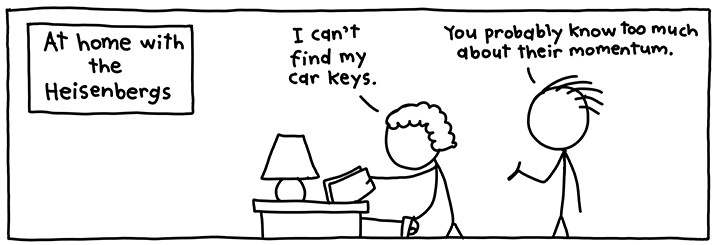
\includegraphics[width=0.7\textwidth]{keys-heis.jpg}
	\caption{Courtesy of \url{www.xkcd.com/824}}
\end{figure}

Most of you have probably heard of the uncertainty principle, as it's one of the more well known parts of quantum mechanics in popular science. As the cartoon above illustrates - one way of stating the uncertainty principle is to say that:
\begin{quote}
	\textit{It is impossible to simultaneously measure the exact position and momentum of a particle}
\end{quote}
Or alternatively, \emph{if we know the position of a particle exactly, then we cannot say anything about it's momentum} (and vice versa). Conceptualising this qualitatively is quite tricky, but we can imagine that a wavefunction where we knew the exact position of a particle would be zero everywhere except for at one well defined position. Such a wavefunction has to be made of combination of a huge number of different wavefunctions that all have different momenta (which is because of something called Fourier Theory, trust me!). Therefore, to have a well defined position, we inherently have a poorly defined momentum. So, if we know the exact position, we don't know anything about the momentum (i.e. we have enormous uncertainty in our measurement of the momentum).

This can be put on a more secure mathematical footing by considering something called a \textbf{commutator}. Two operators are said to \textbf{commute} if the order in which the operators are applied to a system \emph{does not matter}. That is, for two arbitrary operators $\hat{A}$ and $\hat{B}$, with corresponding observables $A$ and $B$:
\begin{equation}
	\hat{A}(\hat{B}\wf) = \hat{B}(\hat{A}\wf)
\end{equation}
These operators \textbf{commute}, and that means that we can \emph{exactly measure both of their corresponding observables simultaneously}. Looking at the equation above, this makes sense, because the equation tells us that it \textbf{doesn't matter if we measure A, then B, or B, then A}. The implication of this is that if measuring A \emph{affected} B, then it would matter in which order we measured them, and the operators would \emph{not} commute. Accordingly, then, the \textbf{position} and \textbf{momentum} operators \textbf{do not commute}, as we \textbf{cannot exactly measure position and momentum simultaneously}, or alternatively \textbf{measuring the position will affect the momentum, and vice versa.} 

A rearrangement of the above equation tells us that if the two operators commute, then $\hat{A}(\hat{B}\wf)-\hat{B}(\hat{A}\wf) = 0$. We can then define the quantity, $\hat{A}\hat{B}-\hat{B}\hat{A} = [\hat{A},\hat{B}]$, which is called a \textbf{commutator}. Specifically $[\hat{A},\hat{B}]$ is the \textbf{commutator of A and B}. If the two operators commute, then their commutator is equal to zero (as in the above case). The commutator of position and momentum $[\hat{x},\hat{p}_x] = i\hbar$ (see above table for definitions of position and momentum operators). The commutator of two operators is non-zero if the operators \textbf{do not commute}. In this case, it is \textbf{impossible to measure the corresponding observables both accurately and simultaneously}.

What does the value of the commutator tell us? It relates to the degree of uncertainty inherent in the measurement \textbf{when we try to measure both observables simultaneously}. Therefore, if the commutator is zero (i.e. the operators of the observables commute), then there is no uncertainty inherent in a simultaneous measurement, and we can accurately measure both observables simultaneously. In the case of a non-zero commutator, the product of the uncertainties associated with each observable is given by:
\begin{equation}
	\Delta A \Delta B \geq \frac{1}{2} \lvert \langle [\hat{A},\hat{B}] \rangle \rvert
\end{equation}
Which, when we plug in the position and momentum operators instead of our arbitrary $\hat{A}$ and $\hat{B}$ operators, leads us to the (maybe!) familiar statement of \textbf{Heisenberg's Uncertainty Principle}:
\begin{equation}
	\Delta x \Delta p \geq \frac{\hbar}{2}
\end{equation}
Plug in the operators and see for yourself!

\section{Summary - The Postulates of Quantum Mechanics}
Before we look at some specific examples this is a good time to take stock and summarise what we know. A lot of the results we've arrived at are referred to as \textbf{The Postulates of Quantum Mechanics}. A \emph{postulate} is just something that is \emph{assumed to be true} - these are the foundations on which quantum mechanics is based. The postulates are considered to be \emph{self-evident}, and aren't independently provable. You could try and argue with them, but this would be a waste of time - they're \emph{self-evident}.\footnote{This starts to get dangerously close to philosophy - and is very much beyond the scope of this course}.

The list below contains most of the postulates - one or two we haven't met as they're outside the scope of what we're currently doing. With each postulate, we'll recap some of what we learnt during this last chapter.

\begin{enumerate}
	\item All dynamical information about a system is contained within the \textbf{wavefunction} of a system. The wavefunction of a system is obtained by solving the \textbf{Schr{\"o}dinger Equation} for that system.
	\item Acceptable wavefunctions have the following properties:
		\begin{enumerate}
			\item They cannot be zero everywhere, or infinite anywhere.
			\item They must be \emph{single-valued} - they cannot contain any points where $\wf(x)$ has multiple values for the same value of $x$.
			\item They must be continuous, and have a continuous slope - with no steps or kinks. This is because it must be possible to compute the \emph{second derivative} of the wavefunction.
		\end{enumerate}
	
	\item The \emph{Born Interpretation} of the wavefunction says that the probability of finding a particle at a certain location is proportional to the square of the wavefunction at that location. 

	\item \emph{Observables} are computed using \emph{operators}, operating on \emph{wavefunctions}. 
		\begin{enumerate}
			\item Observables are quantities we can physically measure, like energy, momentum, position, or even things like dipole moments.
			\item Operators are just mathematical instruction sheets that tell you what mathematics to perform on whatever is being operated on.
			\item Finding the operator that corresponds to a specific observable allows us to calculate the observable for a certain system simply by \emph{operating} on the wavefunction for that system with the operator.
			\item The \emph{Hamiltonian Operator} is a special operator that calculates the observable \emph{total energy}.
		\end{enumerate}
	\item \emph{The Uncertainty Principle} states that it is impossible to specify simultaneously and precisely the momentum and position of a particle. This is because the position and momentum operators do not \emph{commute}.
\end{enumerate}
I hope you followed all this well enough - it probably seems like a lot of things to get your head around! Luckily, we've introduced most of the new concepts already. The subsequent sections will just be applying them to different specific situations. Starting with a simple one - the \textbf{particle in a 1-D box}.
\newpage
\begin{vplace}
	\begin{center}\textbf{\Large{Aside: Solving the Schr{\"o}dinger Equation}}\end{center}
Generally speaking, there aren't really very many systems for which the SE can be \emph{analytically} solved. To solve something \emph{analytically} means to apply algebra and find the exact solution - the equation $x^2 + 1 = 0$ has two analytical solutions (what?). The SE tends to not be analytically solvable (except for some systems which we will see here), so instead needs to be solved \emph{numerically}. 

	Solving something numerically means to make a series of (normally educated) guesses at the solution, and then testing to see how good they are. Then the solutions will be optimised using trial-and-error until an accurate solution is found. This solution will always be an \emph{approximation} to the true solution - but could be within $0.000001\%$ of the true solution! In computational chemistry, this is normally how the SE is solved - as for anything more complicated than a Helium atom (i.e. most things on earth), the SE cannot be analytically solved! 

In the subsequent sections, we will focus our attention on model systems that can be analytically solved - these are educational without having all the extra complexity of having to be solved numerically! These model systems correspond to three kinds of motion that are common in atoms and molecules: \textbf{translational}, \textbf{vibrational}, and \textbf{rotational} motion. We will take each of these systems in turn.  
\end{vplace}
\chapter{Translational Motion}
Translational motion is motion through space. If I pick up a potato and throw it, I am \emph{translating} it's position from my hand to somewhere else. You might then say that the potato gains \emph{translational kinetic energy}. From a more chemical perspective, molecules undergo translational motion as they move around in space - and the amount of translational kinetic energy they have depends on their temperature. We will now describe this motion using the language of quantum mechanics.

\section{Free Motion in 1 Dimension}
In the previous chapter we discussed the Schr{\"o}dinger Equation (SE) ($\hat{H}\wf = E\wf$) and the idea of operators and observables. We saw that the \emph{Hamiltonian operator} is the operator that will produce the observable \emph{total energy} when applied to a wavefunction. If we imagine a particle of mass $m$ moving freely (in no potential, so $V(x)=0$) in one dimension along $x$, it only has kinetic energy. The Hamiltonian, $\hat{H}$ therefore only has one term (a kinetic energy operator), and is given by:
\begin{equation}
	\hat{H} = -\frac{\hbar^2}{2m} \frac{\mathrm{d}^2}{\mathrm{d}x^2}
\end{equation}
Where $\hbar$ is the reduced Planck constant ($\hbar = h/2\pi$). If we call the wavefunction that describes this system \wf, then the SE that describes this system is:
\begin{equation}\label{eq:free_motion}
	-\frac{\hbar^2}{2m} \frac{\mathrm{d}^2\wf}{\mathrm{d}x^2} = E \wf
\end{equation}
Where $E$ is the total energy of the system, which in this case is just the kinetic energy as the potential energy is zero for a free particle. You'll notice that \autoref{eq:free_motion} is a second-order differential equation, and deriving the solutions for this kind of equation is beyond the scope of this course. So you'll need to trust me that the general solutions to this kind of equation, $\wf_k$ can be written as follows:
\begin{equation}\label{eq:general_wavefunction}
	\wf_n = A\cos(kx)+B\sin(kx)
\end{equation}
Where $A$ and $B$ are constants. $k$ is a parameter related to the wavelength of the wave described by~\autoref{eq:general_wavefunction}, the details of which need not detain us here.   

Try to plug $\wf_k$ into \autoref{eq:free_motion}, and you should find the following:
\begin{align}
	-\frac{\hbar^2}{2m} \frac{\mathrm{d}^2\wf_k}{\mathrm{d}x^2} &= -\frac{\hbar^2}{2m} \frac{\mathrm{d}^2}{\mathrm{d}x^2}(A\cos(kx)+B\sin(kx)) \\ &= -\frac{\hbar^2}{2m}(-k^2 A\cos(kx) - k^2 B\sin(kx)) \\ &= \frac{\hbar^2k^2}{2m} (A\cos(kx) + B\sin(kx)) \\ &= \frac{\hbar^2k^2}{2m} \wf_k = E_k\wf_n
\end{align}
So, in this case the total energy of the particle is given by:
\begin{equation}\label{eq:free_motion_energy}
E_k = \frac{\hbar^2k^2}{2m}
\end{equation}
Where we have added the subscript $k$ to denote that this is the energy for an arbitrary value of $k$. Can you see how this is basically just the classical kinetic energy of particle? If not, then think about the general expression for kinetic energy, and how it can be rearranged in terms of linear momentum, $p=mv$.
\begin{equation}
	E_\mathrm{kin.} = \frac{1}{2}mv^2 = \frac{(mv)^2}{2m} = \frac{p^2}{2m}
\end{equation}
So, we can now see that if we take \autoref{eq:free_motion_energy}, and define the momentum of our particle as $p_k = k\hbar$, then we obtain an equation for the kinetic energy that looks like the above! So what does this mean? We've shown that the momentum of our particle along $x$ is given by $p_x = k\hbar$, with it's kinetic energy being given by $E_\mathrm{kin.} = \frac{k^2\hbar^2}{2m}$. Expressing energy and momentum in units of Planck's constant is something that you will become used to throughout quantum mechanics. There are some subtleties that I have deliberately omitted here - if you're very astute you may have noticed that the units of $\hbar$ are \si{\joule\second}, which makes it complicated to see how $k\hbar$ is the linear momentum! For now, you can just consider that $k$ is a constant that allows you to express linear momentum in units of $\hbar$. I'll refer you to Chapter 2 of \emph{Molecular Quantum Mechanics} by Atkins and Friedman if you want to know more. 

One key point here is that we have so far seen \emph{no restrictions on the value of $k$}. Or, in other words - \textbf{the energy of a free particle is not quantised}. This makes perfect sense - as if a particle is free to move wherever it wants to, and have whatever energy it wants to, it doesn't make sense for it to be trapped into discrete, quantised energy states! If I took my potato and threw it, it could have whatever energy I threw it with - it wouldn't be locked into specific energy states. A good analogy for this is imagining two cars, a Quantum Car and a Classical Car. The Classical Car behaves like a car we know - you can accelerate and the speedometer can show any speed between 0 and (around) \SI{140}{\mph}. In contrast, if you drove a Quantum Car, your speedometer would be locked at specific speeds - you could only drive at (for example) 0, 30, 60, 70, or \SI{100}{\mph}. The speeds are \textbf{quantised}.   

\section{Particle in a 1D Box}
Now we move on to a system that you're probably (at least somewhat) familiar with - the \textbf{particle in a one-dimensional box}. This is just like the system above, except that now there are two walls at either end of our region of space - so we don't have completely free movement. The particle isn't allowed to exist outside of the space bounded by the two walls.

Mathematically we can define this situation as follows. We take the $x$ dimension to be the dimension our particle is moving in, and we define three distinct regions of space along $x$. We have an area where the particle can move freely (the interior of the box). As the particle can move freely here, there is no potential energy acting on the particle, so the potential along $x$, $V(x)=0$. We can then define two other regions, where the particle cannot exist - these are the walls of the box. Here, the potential $V(x)$ is infinitely large. We can the define the overall potential as a \textbf{piecewise potential}, as shown below alongside the pictorial representation of the box. 

\begin{minipage}[c]{0.35\textwidth}
	\begin{equation*}
		 V(x) = \begin{cases} 0 &\mbox{if}~ 0\leq x \leq L \\ \infty & \mbox{otherwise} \end{cases}
	\end{equation*}
\end{minipage}
\begin{minipage}[c]{0.64\textwidth}
	\centering
	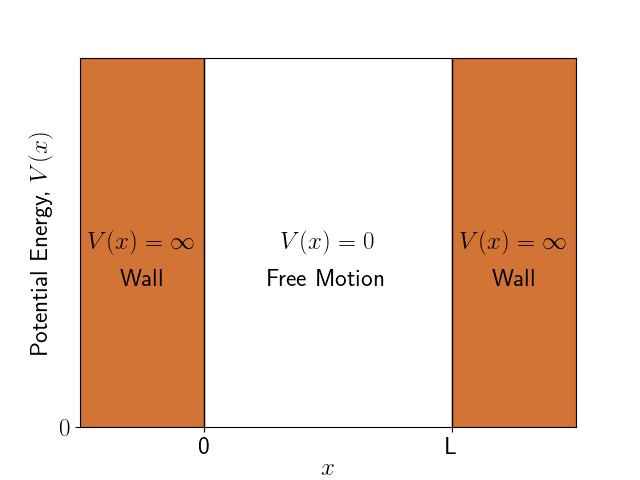
\includegraphics[width=\textwidth]{particle_box_walls.png}
\end{minipage}

Here we have defined our box as being a length $L$, such that the two walls occur at $x=0$ and $x=L$. The piecewise potential shows us that the potential energy is zero between $0$ and $L$ (inside the box - the white area on the figure); and infinite at all other positions (the brown areas on the figure). You might ask why we're interested in this system - and we'll see why later - but it's a useful model system to learn about some of the key aspects of quantum mechanics, and can also be applied to some chemical problems too. 

Let's now look into the mathematics of this system. We can write the SE for this system as follows:
\begin{equation}\label{eq:particle_in_box}
	-\frac{\hbar^2}{2m}\frac{\dd^2\wf(x)}{\dd x^2} + V(x)\wf(x) = E \wf(x)
\end{equation}
This is the same as the SE for a free particle (\autoref{eq:free_motion}), but we've added in the potential $V(x)$, which we assumed was zero everywhere in the case of the free particle. Inside the box, where $V(x)=0$, \autoref{eq:particle_in_box} reduces to \autoref{eq:free_motion}. 

Outside the box, where $V(x)=\infty$, things are a bit more complex. A particle cannot exist with infinite potential energy - to understand this think of an equivalent classical situation: a potato rolling down an infinitely large hill. If a potato was on top of an infinitely large hill, it would have infinite potential energy - as it rolled down, it would eventually gain infinite kinetic energy. This violates all the laws of thermodynamics, because we have perpetual motion, and also an infinitely large hill is obviously a nonsensical thing to think about! \emph{Things cannot have infinite energy!}

Having established that the particle cannot have infinite energy, it therefore cannot exist in a region of infinite potential. Therefore, the wavefunction of the particle \emph{must be zero} when inside the walls (i.e. in either of the brown areas in the picture above). So what form does the wavefunction take inside the box? 

We saw that the SE for the particle in the box (\autoref{eq:particle_in_box}) reduces to the SE for a free particle (\autoref{eq:free_motion}) when we restrict ourselves to only existing between the two walls of the box, between $x=0$ and $x=L$. We already found out the solutions for this situation in the previous section! To recap, the wavefunctions that solve \autoref{eq:particle_in_box} when $V(x)=0$, together with the corresponding energies are:
\begin{equation}\label{eq:pinbox_general}
	\wf_k = A\cos(kx) + B\cos(kx), \qquad E_k = \frac{k^2\hbar^2}{2m}
\end{equation}
Previously we said there were no restrictions on the values of $k$ that were permissible, and therefore there was no quantisation. This is no longer the case due to \textbf{boundary conditions}. 

\subsection{Boundary Conditions and the Emergence of Quantisation}
To quickly recap a salient point, $\wf_k$ \textbf{must be zero inside the walls} - that is when $x<0$ and $x>L$ - else we would have a particle with infinite energy. Additionally, we know that between the walls, $\wf_k$ has a similar form to what we've already seen for a free particle. So we know what happens on either side of the walls. The interesting question is then: \textbf{what happens at the exact point where the wall starts?} Mathematically, we're then considering what happens when $x=0$ and $x=L$. 

\begin{wrapfigure}{r}{0.5\textwidth}
	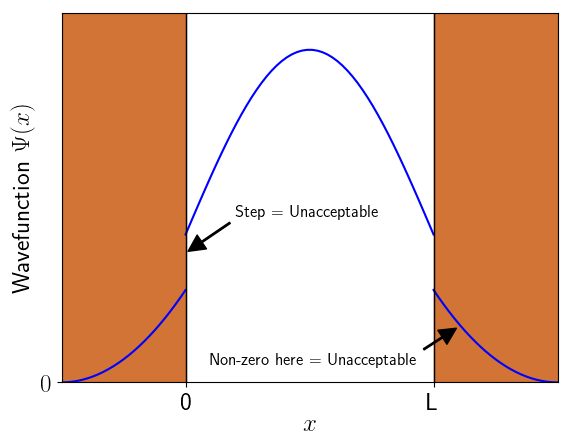
\includegraphics[width=\linewidth]{particle_box_wf_unacceptable.png}
\end{wrapfigure}
It was shown in the first chapter that acceptable wavefunctions have to be \textbf{continuous} - that is, have no steps or kinks in them. This has profound implications for us now, as it tells us that any acceptable wavefunction for this system \textbf{must be zero} when $x=0$ and $x=L$ - or more mathematically, $\wf_k(0) = \wf_k(L) = 0$. These are called our \textbf{boundary conditions} - they tell us \emph{what happens at the boundaries} of our system. The adjacent figure shows a wavefunction for our box which doesn't obey our boundary conditions - showing a clear step at the wall of the box, making it an unacceptable wavefunction. It also isn't zero when it's inside the walls - making it doubly unacceptable!

So what do the \emph{acceptable} wavefunctions look like? Let's start with our general expression for the form of the wavefunctions, $\wf_k(x)$:
\begin{equation}
	\wf_k = A\sin(kx) + B\cos(kx)
\end{equation}
We said that $\wf_k(0) = 0$ and $\wf_k(L) = 0$. Let's apply the first of these boundary conditions initially:
\begin{equation}
	\wf_k(0) = A\sin(k(0)) + B\cos(k(0)) = B\cos(0) = B = 0
\end{equation}
Where we have used the fact that $\sin(0) = 0$ and $\cos(0) = 1$ (and that anything multiplied by zero is zero). So this tells us already that $B=0$, so we have no cosine term in the true wavefunction. We can now apply the second boundary condition, $\wf_k(L) = 0$, knowing that $B=0$.
\begin{equation}
	\wf_k(L) = A\sin(kL) = 0
\end{equation}

\begin{wrapfigure}{r}{0.5\textwidth}
	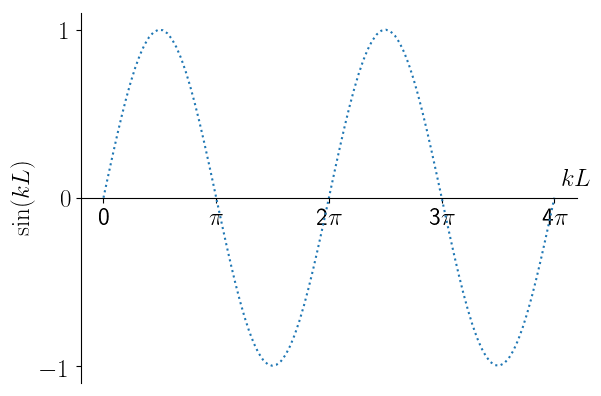
\includegraphics[width=\linewidth]{boundary_conditions_pinbox.png}
\end{wrapfigure}
Now we have to be a bit cleverer. We know that $L$ is a constant and is just the length of our box, so what values of $k$ do we have to pick such that $\sin(kL)=0$? To do this, consider the graph of $\sin(kL)$ against $kL$ plotted on the right - it should be clear that $\sin{kL}$ is equal to zero only when $kL$ is equal to \emph{integer values of $\pi$}. So we can write:
\begin{equation*}
	kL = n\pi, \qquad  n=0,1,2,3...
\end{equation*}
And a simple rearrangement then tells us that:
\begin{equation*}
	k = \frac{n\pi}{L}, \qquad n=0,1,2,3...
\end{equation*}
That is, there are only \emph{certain, discrete values of $k$ that give us an acceptable wavefunction}. So knowing this, and knowing that $B=0$ from our first boundary condition, allows us to write our overall wavefunction $\wf_n(x)$ as follows:
\begin{equation}
	\wf_n(x) = A\sin\bigg(\frac{n\pi x}{L}\bigg), \qquad n = 1,2,3,4...
\end{equation}
This is the general form of a wavefunction for a particle in a 1D box! Note that we have changed the subscript $k$ to a subscript $n$. Let's recap what each symbol means. $A$ is just a constant, and is actually the \emph{normalisation constant} - this was mentioned in the previous chapter. $L$ is simply the length of the box we have, $x$ is our position inside the box, $\pi$ is a constant, and $n$ is something called a \textbf{quantum number}. A quantum number is just a number (generally an integer but not always) which tells us \emph{which state of the system we are currently in}. You'll hopefully have spotted that even though $n=0$ satisfies our requirement for $\sin(kL) = 0$, it would actually result in an unacceptable wavefunction (because then $\wf_k(x) = 0$ everywhere, which is not allowed!), so our lowest quantum number is actually $n=1$. 

Before we look at what the wavefunctions actually look like, remember that in \autoref{eq:pinbox_general} we also had an expression for the energy of our particle, that depended on the value of $k$. Now we actually know what $k$ is, we can write a more precise definition of the energy of our particle, $E_n$ (remembering that $\hbar = \frac{h}{2\pi}$):
\begin{equation}
	E_n = \frac{(\frac{n\pi}{L})^2\hbar^2}{2m} = \frac{n^2\pi^2\hbar^2}{2mL^2} = \frac{n^2\pi^2h^2}{8\pi^2mL^2} = \frac{n^2h^2}{8mL^2},\quad\text{where:} n=1,2,3... 
\end{equation}
Can you see how this gives us a \emph{discrete, quantised set of energies?} As $n = 1,2,3...$, our only acceptable energies are obtained by plugging integer values of $n$ into this formula! What this is telling us is that \emph{the particle can only exist in the box with specific, discrete energies.} This is massive, as we've now \textbf{quantised} our energy! Furthermore, \textbf{the quantisation arose because we added boundary conditions} - the free particle with no walls was not quantised - so the presence of the walls creates the quantisation. Welcome to quantum mechanics!

\subsection{The Acceptable Solutions}
We are now in a position to write down the acceptable solutions of the SE for particle confined to a 1D box. However, we have neglected one thing, and that is to normalise our wavefunction - to find a value for the constant $A$. This will be left as an exercise for you (it isn't very difficult!), just remember that the definition of normalisation is:
\begin{equation}
	\int_{-\infty}^\infty \wf^2 \dd x = 1
\end{equation}
And in this case, the only space our particle has to exist in is between $x=0$ and $x=L$ - so we can rewrite our integral as follows:
\begin{equation}
	\int_0^L \wf^2 \dd x = \int_0^L A^2 \sin\bigg(\frac{n\pi x}{L}\bigg)^2 \dd x = 1
\end{equation}
If you evaluate this integral (go on!) and solve for $A$\footnote{Remember that for an acceptable solution $n$ is an integer.}, then you should find that:
\begin{equation}
	A = \sqrt{\bigg(\frac{2}{L}\bigg)}
\end{equation}
This allows us to write down the full set of solutions to the SE for this system:
\begin{myblock}{\begin{center}Particle in a 1D Box\end{center}}
	\begin{center}
		\begin{align*} & \text{\textbf{Hamiltonian}} \qquad\qquad \hat{H} = -\frac{\hbar^2}{2m}\frac{\dd^2}{\dd x^2} + V(x),\quad  \text{where} \quad V(x) = \begin{cases} 0 &\mbox{if}~ 0\leq x \leq L \\ \infty & \mbox{otherwise} \end{cases} \\
	& \text{\textbf{Schr{\"o}dinger Equation}} \qquad\qquad -\frac{\hbar^2}{2m}\frac{\dd^2\wf_n(x)}{\dd x^2} + V(x)\wf_n(x) = E_n \wf_n(x) \\
		& \text{\textbf{Wavefunctions}} \qquad\qquad \wf_n(x) = \sqrt{\bigg(\frac{2}{L}\bigg)}\sin\bigg(\frac{n\pi x}{L}\bigg), \quad \text{for} \quad 0 \leq x \leq L \quad\text{and}\quad n = 1,2,3... \\ 
		& \text{\textbf{Energies}} \qquad\qquad\qquad\qquad\qquad\qquad\quad E_n = \frac{n^2h^2}{8mL^2}, \quad \text{where} \quad n = 1,2,3...
	\end{align*}
	\end{center}
\end{myblock}


\begin{wrapfigure}{r}{0.5\textwidth}
	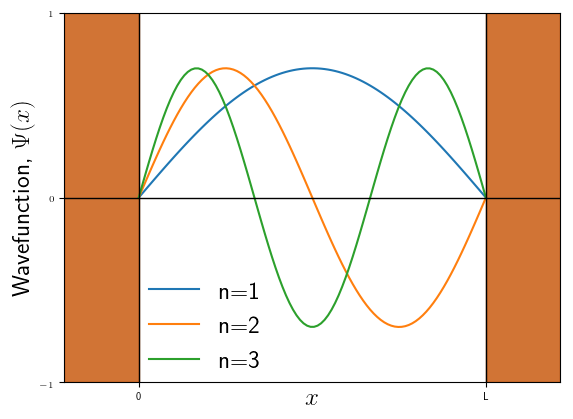
\includegraphics[width=\linewidth]{particle_in_box_wf.png}
	\caption{The first three normalised wavefunctions of the particle in a 1D box. As $n$ increases, the wavelength of the wave in the box decreases, and the energy increases.}
\end{wrapfigure}
So what do these actually look like? The figure to the right shows the first 3 wavefunctions (corresponding to $n=1,2$, and $3$), plotted inside the box. You can see that the lowest energy wavefunction, \wf$_1$, is only zero at the edges of the box, and has no other internal \textbf{nodes}. A \textbf{node} is a place where the wavefunction passes through zero. As you increase the value of the quantum number $n$, you can see that the number of nodes increases - by one each time. Higher energy wavefunctions \emph{have more nodes}. We can rationalise this as follows.

Consider each wavefunction as a \emph{standing wave} within the box - you may have seen standing waves in physics lessons in school. Standing waves occur when you can fit a half-integer number of wavelengths \emph{exactly} into the length of the box, and if the box was something like a flute, each standing wave is a different musical note. In this case, $n=1$ gives the first standing wave, and $n=2$ has fitted an extra half-wavelength in, and so on for $n=3$. As we do this, we can see that the \emph{wavelength of each standing wave is decreasing as the quantum number, n, increases}. Wavelength is inversely proportional to energy - shorter wavelengths mean higher energies, and higher quantum numbers mean shorter wavelengths, so higher quantum numbers must mean higher energies. 

\begin{wrapfigure}{l}{0.28\textwidth}
	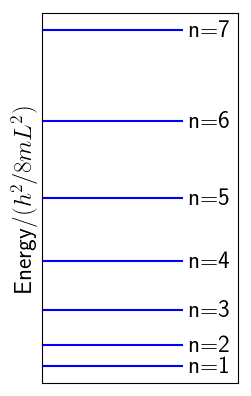
\includegraphics[width=\linewidth]{particle_in_box_energies.png}
	\caption{The first six energy levels for a particle in a 1D box.}
\end{wrapfigure}
It's useful now to consider the actual energies in more detail. The diagram to the left shows the first six energies of the particle in a 1D box, plotted relative to each other. Here we can see several interesting things. Firstly, the particle cannot have zero energy, and the lowest energy is given by $E_1$, when $n=1$. This is called the \textbf{zero-point energy}, and is the lowest energy a particle can have. This means that the particle cannot be stationary, with zero energy, as would be allowed classically. This zero-point energy cannot be removed. We can understand the zero-point energy in the context of the uncertainty principle (remember that this is an entirely quantum phenomenon and so a nice classical analogy involving potatoes isn't available here!). 

If a particle is confined to finite region (as in this case), it's position \emph{must be known} to some degree of precision - i.e. \emph{the particle must be in the box}. The Uncertainty Principle tells us that a particle can only have an absolutely precisely defined energy if the position is completely undefined. Therefore, for the energy to be zero (and exactly zero), it's position must be \emph{completely undefined}, which is not the case as we know the particle must in the box! Hence, a particle in a box always has to have some energy, even at the lowest quantum number, and this is the zero-point energy.

We can also look at the separation of adjacent energy states - it is clear from the diagram that the separation of two adjacent states increases as $n$ increases. We can learn more by considering the value of the energy spacing, $\Delta E = E_n - E_{n+1}$.
\begin{equation}
	\Delta E  = E_n - E_{n+1} = (2n+1)\frac{h^2}{8mL^2}
\end{equation}
Here we can clearly see what we previously observed, that a larger value of $n$ will result in a larger value of $\Delta E$. What we can also now consider is the effect of increasing or decreasing the width of the box, $L$. Consider the case where $L = 0$, here $\Delta E$ is infinitely large, and the particle cannot exist (obviously, because if $L=0$ there is no box). More interesting is the case where $L$ is infinitely large - $\Delta E$ will tend towards zero as $L$ tends towards infinity. This is a pleasant result, as if we make the box infinitely large, the spacing between adjacent energy states is zero, and the particle isn't quantised any more! This is what we observed at the start of this chapter, when we considered the energy of a particle free to move in one dimension.

\subsection{Probability Distributions and the Correspondence Principle}
We know from the \textbf{Born Interpretation} of the wavefunction that the probability of finding a particle at a point $x$ is proportional to the square of the wavefunction at $x$, $\lvert \wf(x) \rvert^2$. Now we have found some actual real-life wavefunctions, we can look at what these probability distributions look like in practice. If we take our generic particle-in-a-box wavefunction and square it, we obtain the following:
\begin{equation}\label{eq:pinbox_probability}
	\lvert \wf_n(x) \rvert^2 = \frac{2}{L}\sin^2\bigg(\frac{n\pi x}{L}\bigg)
\end{equation}
Simply analysing the form of \autoref{eq:pinbox_probability} tells us a few things. Firstly, that the probability distribution depends on how big the box is (as it depends on $L$) - this makes sense, as the bigger the box, the more places there are to find our particle! Secondly, it depends on the position in the box, $x$, so the probability isn't uniform for the entire box (i.e. we might be more likely to find it in certain positions than others). Finally, it depends on our quantum number, $n$, which means that \emph{the probability distribution for a particle depends on the energy state it's in} - this is key, as we will see shortly. 
\begin{figure}[h]
	\centering
	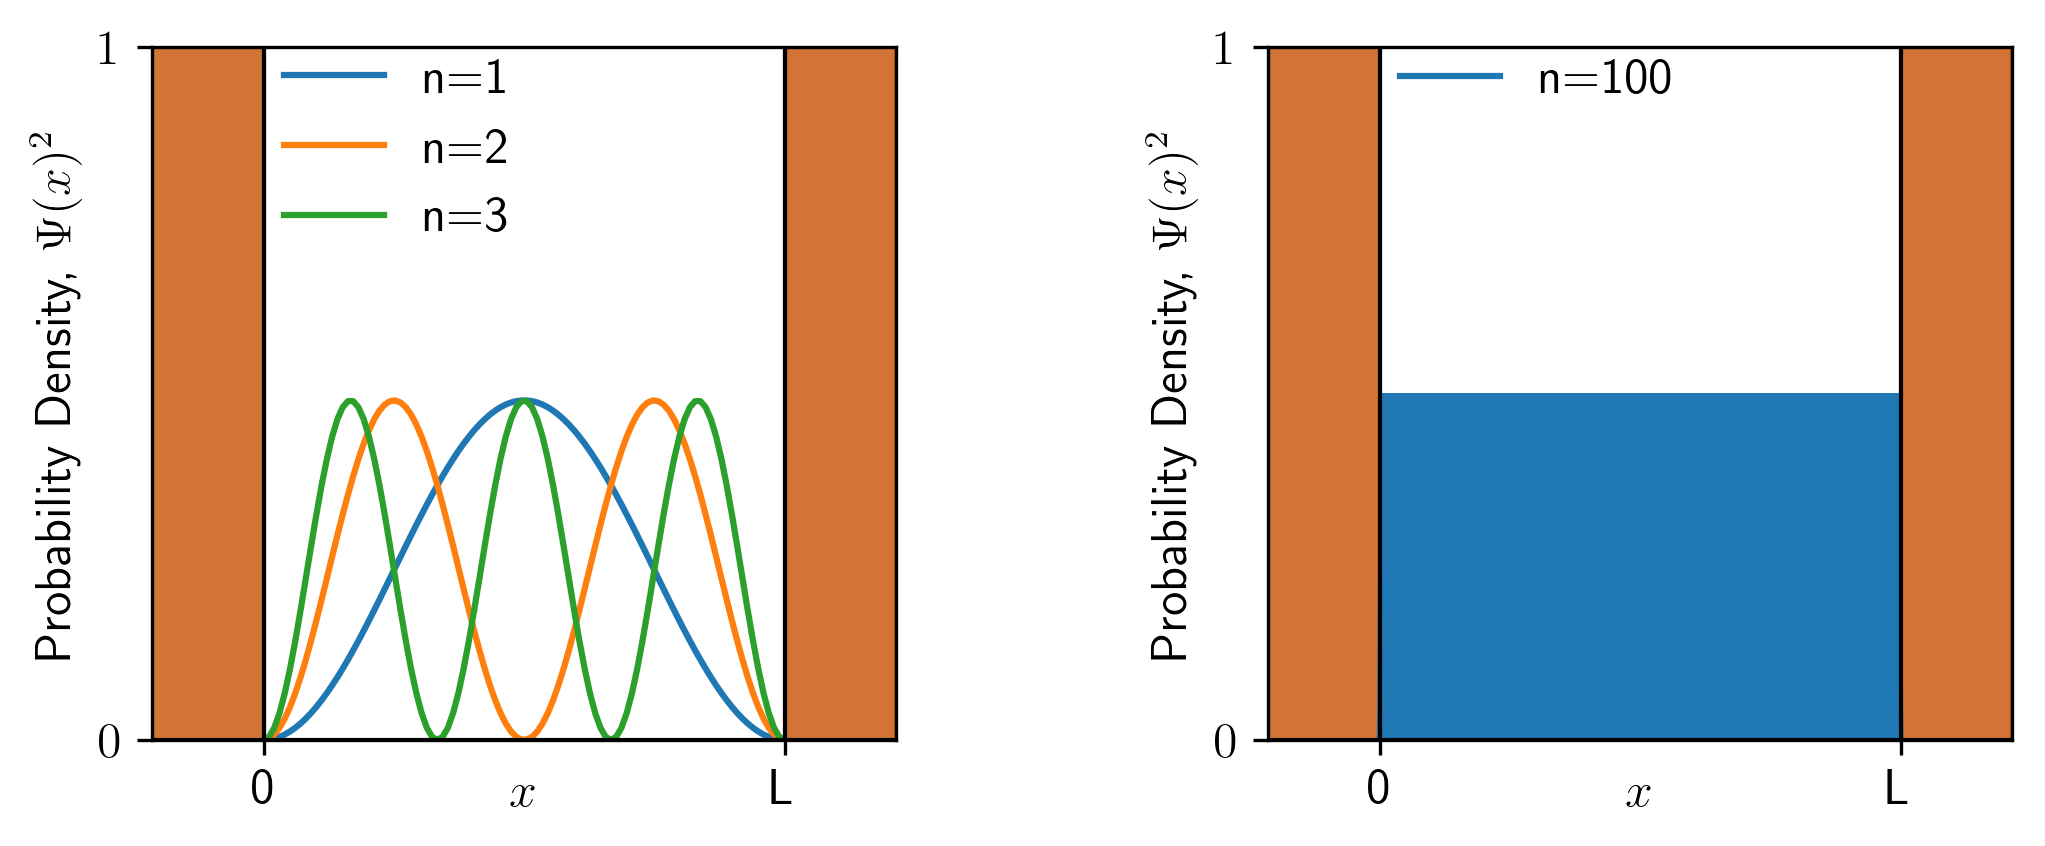
\includegraphics[width=0.7\textwidth]{particle_in_box_probabilities}
	\caption{Left: the probability densities for the particle in a 1-D Box for the first three energy levels. Right: the probability density for the hundreth energy level.}\label{fig:pinbox_probabilities}
\end{figure}

Plotted in \autoref{fig:pinbox_probabilities} are the probability density distributions for the particle in a 1D box at a variety of different values of $n$. On the left, we see the probability distributions for the first three values of $n$. For $n=1$, you can see that the particle is more likely to be found in the middle of the box than at the edges - this is bizarre to think about classically! As we increase to $n=2$ , there's an extra \textbf{node} in the center, and the particle is now more likely to be found nearer the edges - even more bizarre! As we increase to $n=3$, we get another node, and now there are three areas of high probability, at the center, and near the two edges.

This is all quite strange, but it helps to think about what we would expect \emph{classically}. If I gave you a box, and put a potato in it, and then asked you where in the box it was likely to be, you'd reply saying that it could be anywhere - that \emph{all positions are equally likely}. Classically, this is exactly what we would expect - a potato in a box isn't more likely to be in the middle than at the edges! Now, think about what we see in the leftmost figure as the quantum number $n$ increases. At low quantum numbers, the particle spends most time in the middle of the box. As the quantum number is increased, can you see that the probability density spreads out across the box? By $n=3$, there are three regions of high probability spread across the box. If I went to $n=5$, I would see 5 regions of high probability. What if I went to really high quantum numbers?

This is what the rightmost figure shows! If we go to a really high quantum number, $n=100$ in this case, then the \emph{probability distribution is evenly spread across the whole box}. That is, at high quantum numbers, the system behaves \emph{exactly as we would expect a classical system to behave!} This is beautiful, and is an example of the \textbf{quantum-classical correspondence principle}. One way of stating the correspondence principle is to say:
\begin{quote}
	\textit{``Classical mechanics and Quantum mechanics give the same answer at large quantum numbers''}
\end{quote}
Large quantum numbers occur when things are big (i.e. not atoms), or when things are hot (and room temperature is really hot compared to most of the universe!). So, in the limit of things being macroscopic and warm: \textbf{quantum mechanics turns into classical mechanics, almost magically}. Isn't this astounding? You can derive all of Newton's laws from quantum mechanics if you make the quantum numbers big enough! If you're not amazed by this, then I can't help you!

\section{Chapter 2 Summary}
What I want you to take away from this chapter:
\begin{itemize}
	\item The motion of a \textbf{free particle} is \textbf{not quantised}.
	\item \textbf{Quantisation} of a system appears when we add in \textbf{boundary conditions}. In this chapter, we saw that confining a particle moving with translational energy into a \textbf{box with infinite potential at the walls} meant that the energies of that particle became \textbf{quantised}.
	\item For a \textbf{particle in a box}, the \textbf{quantum number} that defines the energy state of the system is $n$. Higher values of $n$ correspond to higher energies.
	\item The energy spacing between two adjacent levels with quantum numbers $n$ and $n+1$ \textbf{increases} as the quantum number is increased. The same spacing will \textbf{decrease} if we make the box bigger, and if the box is \textbf{infinitely big} then the particle is \textbf{not quantised}.
	\item The \textbf{probability distribution} of the particle in a box is confined at low quantum numbers, but at large quantum numbers starts to behave classically. This is an example of the \textbf{quantum-classical correspondence principle}.
\end{itemize}
In the next chapter, we will look at the same situation (a particle with only translational energy), but now our potential is not defined by the walls of a box, but by a \textbf{harmonic oscillator.}

\chapter{Vibrational Motion}
We will now approach a more complicated problem - that is when our particle is confined in a \textbf{harmonic well}. This situation is analogous to that of a vibrating molecule (as we will see later). The mathematics of this problem quickly become too complex for this course - so I have been rather brief with several things. If you want to know more, look in Chapter 2 (and Further Information 2.2) of \emph{Molecular Quantum Mechanics} by Atkins and Friedman.

\section{The Classical Harmonic Oscillator}
You may be familiar with the idea of a \emph{harmonic oscillator}, perhaps from A-Level physics. To understand what it is, consider a spring which is attached to a fixed point, which we are holding at a position \emph{where the spring is completely at rest} - we are not stretching or compressing the spring at all. Let us call this point $x=0$ (the origin), where $x$ is the displacement of the spring. 

If we pull the spring away from $x=0$, perhaps to a point $x=1$, the spring will be resisting our pulling force, and will want to return to $x=0$. We can say here that the we are experiencing a \emph{restoring force}, the spring is trying to \emph{restore} itself back to $x=0$. The magnitude of this force depends on how hard we pull on the spring. If we only pull the string very slightly, it isn't very difficult to do (the restoring force is small). However, if we pull the spring violently, and try to stretch it to many times its original length, we will find that the more we pull it, the more the spring seems to resist. That is, the \emph{restoring force is proportional to how much we displace the spring by}. This is the basis of \textbf{Hooke's Law} (given below) and is illustrated in the picture below. 

\begin{minipage}{0.3\textwidth}
\begin{equation}
	F_R = -k_f x
\end{equation}
\end{minipage}
\hspace{2cm}
\begin{minipage}{0.6\textwidth}
	\centering
	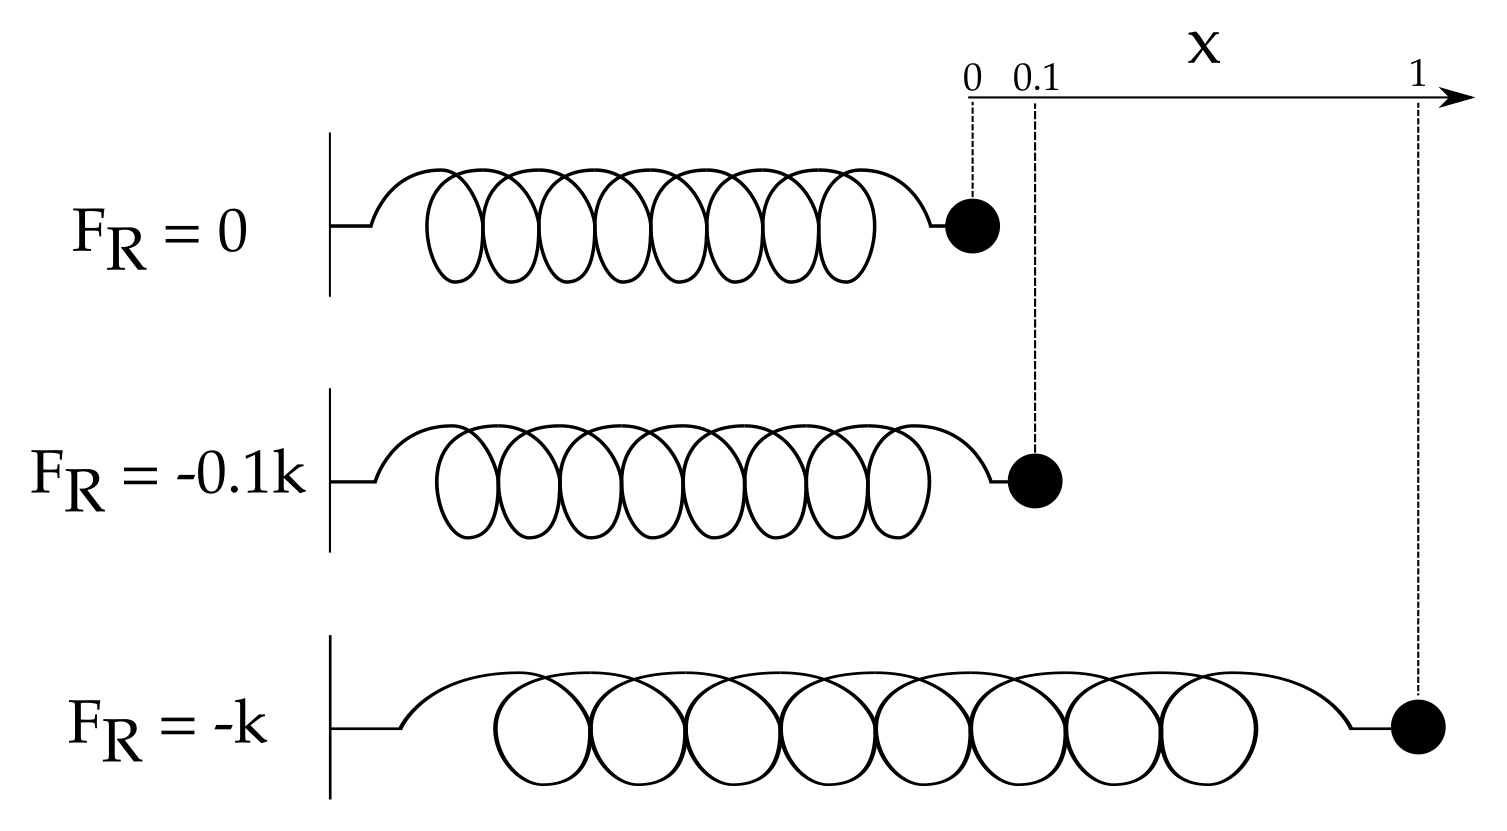
\includegraphics[width=0.7\textwidth]{hooke_law.png}
\end{minipage}

Here $F_R$ is the restoring force, $k_f$ is a constant known as the \textbf{force constant} or \textbf{spring constant} of the spring, and $x$ is the displacement of the spring from it's rest position at $x=0$. The restoring force is always negative, because the force is \emph{pulling us back towards the origin}. As the illustration shows, a larger value of $x$ leads to a larger restoring force. The \textbf{force constant} can be thought of as a proportionality factor between the \emph{restoring force} and the \emph{displacement}. A large value for $k$ means that the spring is very stiff, and we experience a high restoring force for a small pull on the spring. Conversely, a small value of $k$ would mean our spring is quite slack, and we would need to pull on the spring a lot to get a high restoring force. This is illustrated in~\autoref{fig:harmonic_potential}\,(a). 

An obvious extension to this discussion is to start to think about the \emph{potential energy}, $V(x)$, that an object on the end of our spring would have as we pull the spring. Intuitively it makes sense that if we pull the spring so that our object gets further away from $x=0$, then the \emph{potential energy} of the object must increase. We are \emph{doing work} on the object to pull it away from $x=0$, so we are giving it a potential energy that is \emph{proportional to the force we have to overcome to pull it}. The amount of energy it gains is equal to the work we had to do to pull it away from the origin - the further we pull it (or the stiffer the spring (larger $k$)), then the more work we have to do, and the more potential energy it gains. Mathematically, the potential energy $V(x)$ is given by\footnote{You may remember from mechanics that $\text{Work} = \int \text{Force} \,\,\mathrm{d}x$ (work is force times distance) - this is the same equation, except now we have a negative sign because we are now doing work \emph{against} the force, the force isn't doing work \emph{on} us.}:
\begin{equation}
	V(x) = -\int_{x=0}^{x} F_R \,\mathrm{d}x = -\int_{x=0}^{x} -k_fx \,\mathrm{d}x = \frac{1}{2}k_fx^2
\end{equation}
This is an expression for the \textbf{potential energy of a particle trapped in a harmonic well}. To illustrate why we call this a harmonic \textbf{well}, \autoref{fig:harmonic_potential}\,(b) shows a plot of $V(x)$ against $x$. You can see the characteristic parabolic `well' shape - and as the particle moves away from the center of the well, it gets more and more energy - so will tend to want to `roll' back down to the center of the well if it can. 

\begin{wrapfigure}{r}{0.55\textwidth}
	\vspace{-0.5cm}
	\centering
	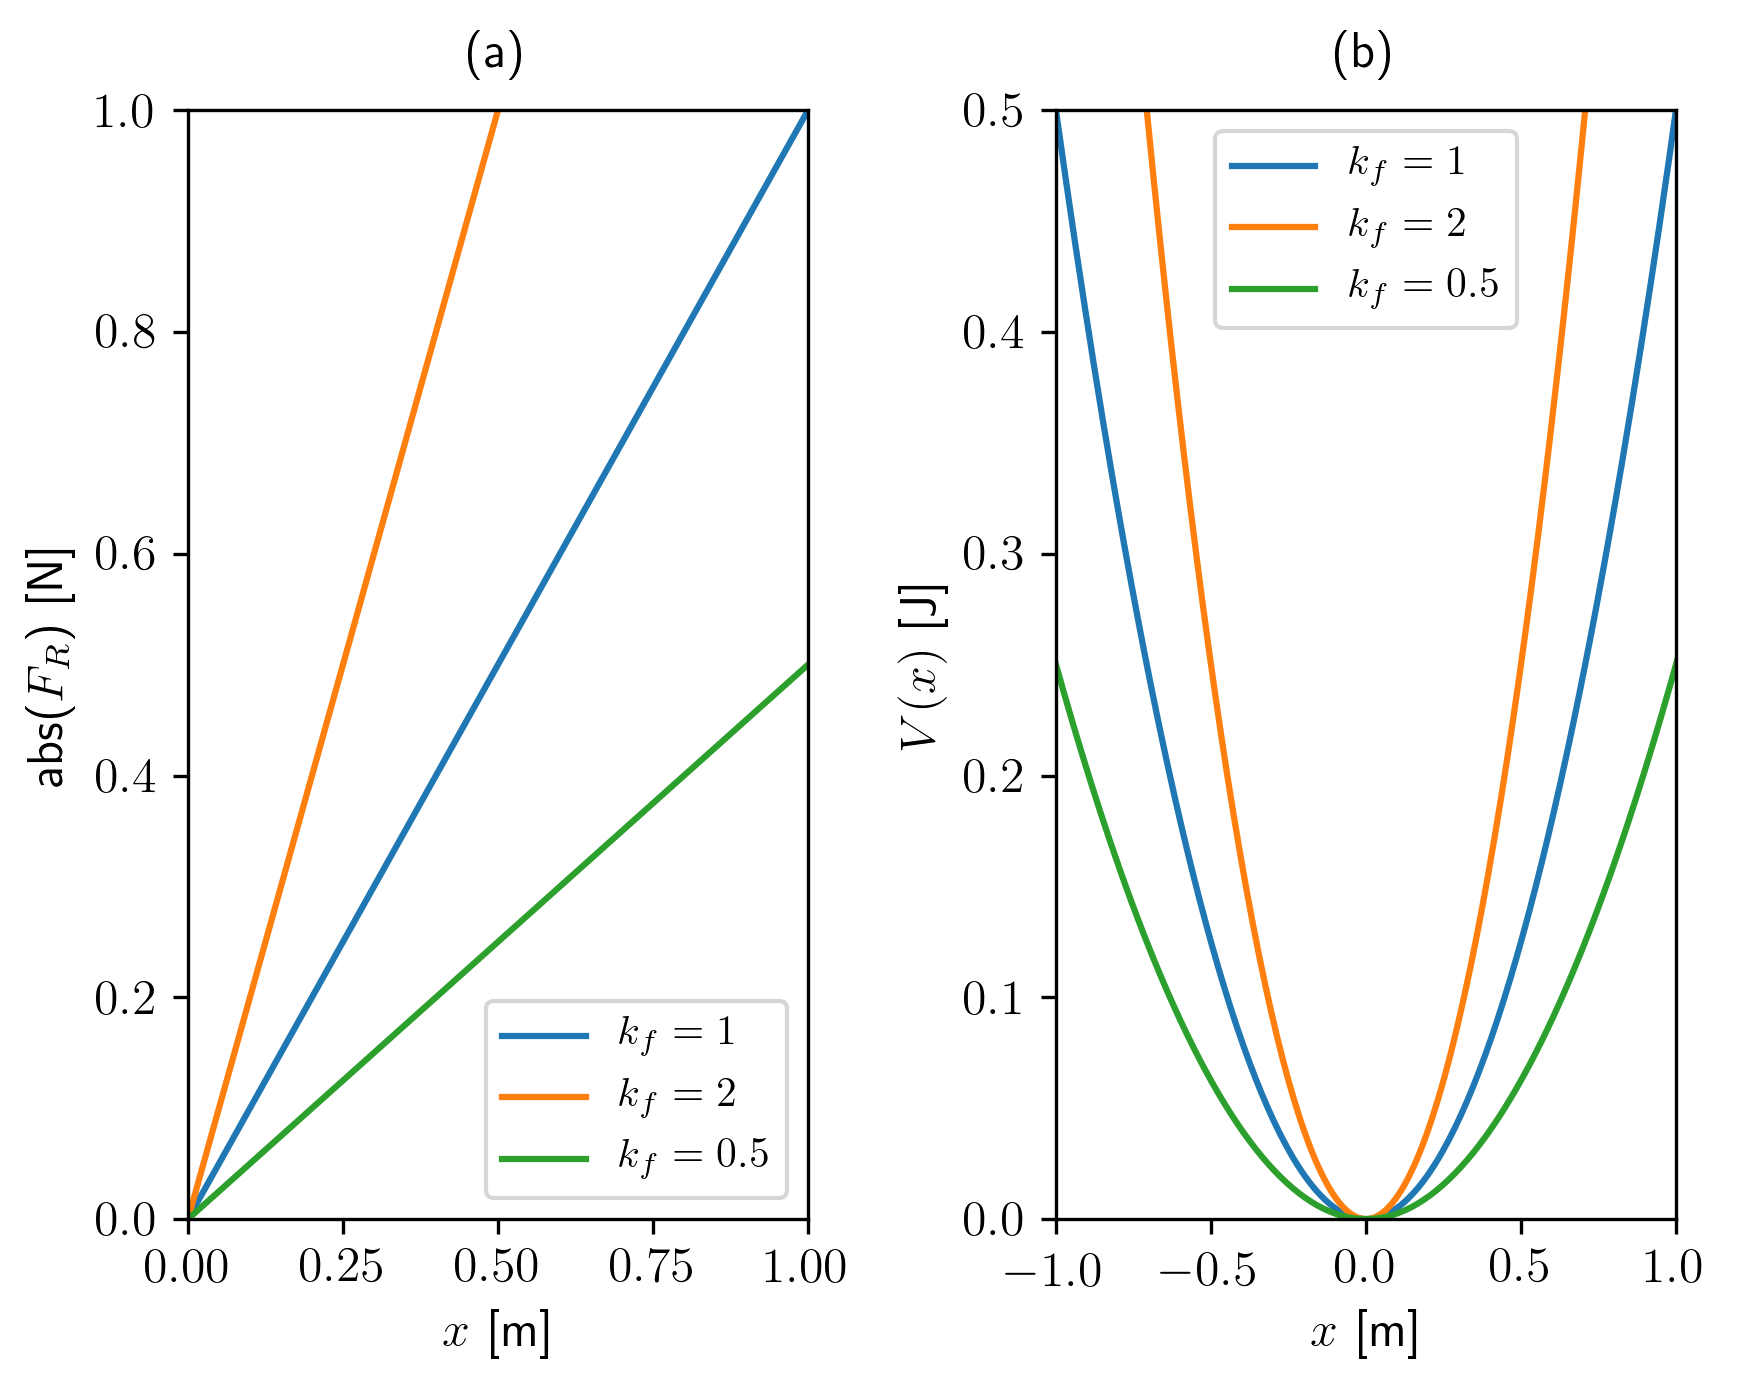
\includegraphics[width=\linewidth]{harmonic_well}
	\caption{(a) The magnitude of the $R_F$ as a function of $x$ for different force constants $k$. (b) As (a), but now the potential energy $V(x)$ rather than $R_F$. Note the characteristic well shape.}\label{fig:harmonic_potential}
\end{wrapfigure}

The figure to the right shows the magnitude of $R_F(x)$ (a) and the potential energy $V(x)$ for a variety of different force constants. Note that the magnitude of $R_F(x)$ is plotted - as $R_F$ is a negative quantity (directed back towards $x=0$), plotting the magnitude makes it easier to visualise. Clearly, the restoring force increases as the spring is stretched (as $x$ increases). Additionally, a larger value of $k_f$ gives a bigger restoring force for a given spring extension - as expected. 

Turning to (b), we can see the characteristic parabolic well shape. Clearly, the further away we are from the origin, the more energy we have - imagine a particle placed at $x=0.5$, it will tend to want to roll down towards $x=0$, converting PE into KE. Varying the force constant here affects how steep the sides are - how \emph{tight} the well is. At low values of $k$, the well is shallow and a particle placed at the edge would roll gently towards the middle. At higher values of $k$, the walls are steeper, and a particle at the edge would roll very fast towards the middle. 

So we have established an expression for the \emph{restoring force} a particle experiences if it is attached to a spring that is stretched, and have derived the \emph{potential energy} that such a particle feels. We haven't actually discussed what \textbf{harmonic motion} is, or why it's called a \textbf{harmonic} well!

Simply, a particle undergoes \textbf{harmonic motion} if it experiences a restoring force proportional to some displacement, as in Hooke's law. So a particle on the end of an oscillating spring is undergoing \textbf{harmonic motion} - and the whole system can be described as an \textbf{harmonic oscillator}. It's called an oscillator because the particle would \emph{oscillate} back and forth very quickly, as it rolls up and down the potential. Think about holding a marble at the top of one of the curves in \autoref{fig:harmonic_well}\,(b) - it would roll down, through the origin, up the other side, and back again - and continue doing so forever in the absence of any friction. This is what \textbf{harmonic motion} is. Another classic example of something which undergoes harmonic motion is a \textbf{pendulum} - we will talk about that a bit more later in the context of the zero-point energy. 

But why is it called \emph{harmonic} motion? This is because if we traced the displacement of that marble onto a piece of paper, or attached a pen to the bottom of a pendulum and dragged some paper under it as it swung, the resulting pattern would look like a sine wave. This is why it's called \emph{harmonic}, because the sine wave could be played as a sound - and would be a single frequency, making a musical note. An exercise left to you is to solve the system below, obtained by equating Newton's Second law and Hooke's law\footnote{Note that $a = \frac{\dd^2x(t)}{\dd t^2}$.}:
\begin{equation}
	ma = -kx
\end{equation}
And derive an expression for the displacement as a function of time, $x(t)$ - this will have the form of a sine or cosine function, as expected! 

\section{The Quantum Harmonic Oscillator}
At this point, after all the physics in the previous section, you're probably asking: ``I'm doing a Chemistry degree, why is all this relevant?''. To which the answer is firstly that science is no respecter of the artificial boundaries set up by University Admissions Departments, and secondly that \textbf{we can model a vibrating molecule as a harmonic oscillator}. We will see exactly how this modelling works later, but first we need to apply the harmonic oscillator potential to our quantum system.

%\subsection{Reduced Mass}
%Imagine a molecule like hydrogen iodide, \ce{HI}. The iodine is about 127 times more heavy than the hydrogen. To all intents and purposes, the hydrogen behaves as if it is pegged to a stationary iodine atom - think of it like a ball and chain. The iodine is an exceptionally heavy ball, and the hydrogen is an exceptionally light criminal. The chain is the chemical bond, which actually behaves \textbf{quite like a spring} under a lot of conditions. So if we wanted to think about the vibration of an \ce{HI} molecule, we can imagine it a bit like a hydrogen atom attached to a wall by a spring - exactly the situation we just described classically in the previous section! 

%We can actually extend this analysis a bit, and say that for \emph{any} diatomic molecule, we can imagine it as a single atom of mass $\mu$ attached to a stationary wall. In this case, $\mu$ is a quantity called the \textbf{reduced mass} - this will be used a lot in this section and also most of the following sections! The reduced mass is defined as:
%\begin{equation}
%	\mu = \frac{m_1 m_2}{m_1 + m_2}
%\end{equation}
%The idea just described is shown in the figure below. For something with a huge difference in mass like \ce{HI}, the reduced mass is basically just $m_H$, because $m_H + m_I \approx m_I$, and therefore $\mu \approx m_H m_I / m_I = m_H$. Where the mass difference isn't so enormous, we can just calculate the reduced mass in accordance with the equation above. Just be aware that reduced mass is a thing that we can use!
%\begin{figure}
%	\centering
%	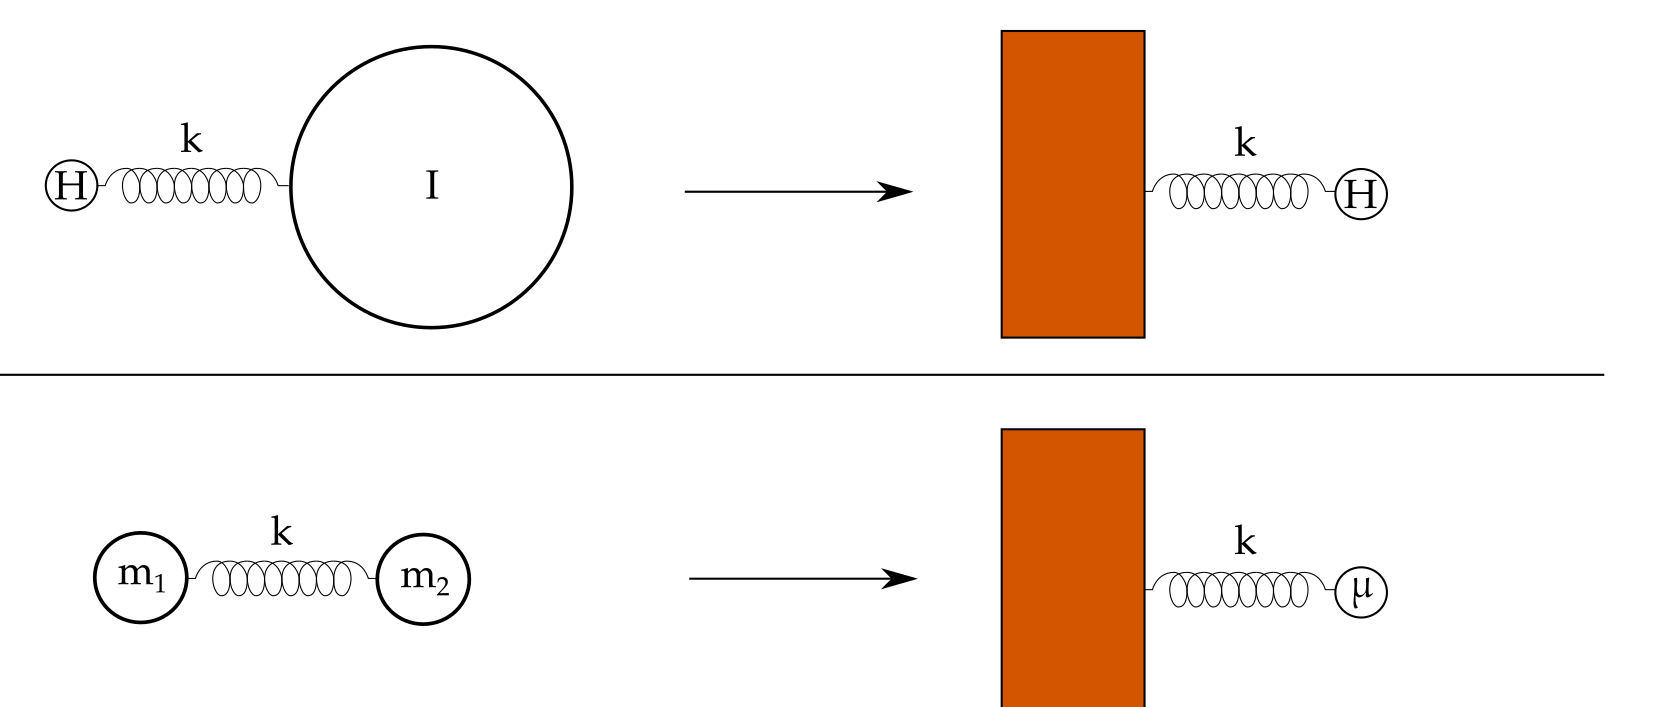
\includegraphics[width=\textwidth]{reduced_masses}
%\end{figure}

\subsection{The SE for a Harmonic Oscillator}
In the previous section, we showed that the potential energy $V(x)$ of a harmonic oscillator was given by:
\begin{equation}
	V(x) = \frac{1}{2} k_fx^2
\end{equation}
Where $k_f$ is the force constant. We can construct the SE for the system quite simply, by making our potential term equal to the equation above, such that our Hamiltonian, $\hat{H}$, is given by a sum of kinetic and potential energy terms:
\begin{equation}
	\hat{H} = -\frac{\hbar^2}{2m}\frac{\mathrm{d}^2}{\mathrm{dx}^2} + \frac{1}{2}k_fx^2
\end{equation}
Our overall SE is therefore given by:
\begin{equation}\label{eq:vibrational_SE}
	-\frac{\hbar^2}{2m}\frac{\mathrm{d}^2\wf_v}{\mathrm{dx}^2} + \frac{1}{2}k_fx^2\wf_v = E_v\wf_v
\end{equation}
Where the subscript $v$ denotes that we are now looking at \emph{vibrational} wavefunctions and energies.

The mathematics behind the solution to this equation are quite complex and beyond the scope of this course - it relies on finding a way to factorise the Hamiltonian which results in the creation of two new operators called \emph{creation and annihiliation operators}. If you're interested, look in Further Information 2.2 in \emph{Molecular Quantum Mechanics}. Without getting detained by the algebra, we can look at the solutions and their properties. 

\subsection{The Vibrational Energy Levels}
Considering first the energy levels $E_v$, these can be shown to given by:
\begin{equation}\label{eq:vibrational_energies}
	E_v = (v+\frac{1}{2})\hbar\omega\,,\quad \text{where:}\quad \omega = \sqrt{\frac{k_f}{m}},\quad\text{for}\, v=0,1,2,3...
\end{equation}
Here $v$ is our \textbf{vibrational quantum number}, and is a way of labelling which of the \textbf{vibrational energy levels} we are in. Note again that our energies are \textbf{quantised} - we can only solve the SE in~\autoref{eq:vibrational_SE} for \textbf{specific energies} - these energies ($E_v$) are given by the equation above, for integer values of $v$. This is very similar to the situation in Chapter 2, for a particle in a box. We saw there that when we added in a non-zero potential, our energies became \textbf{quantised} - the same thing is happening here. If I removed the harmonic potential ($V(x)=0$), we would be back to having a free particle. The main difference here is that now we are \emph{allowed to have an energy level with $v=0$} - previously this was forbidden because for a particle in a box, the energy level where $n=0$ had a wavefunction which was zero everywhere, which isn't allowed. More on this in the following sections. 

Turning back to the rest of the terms in~\autoref{eq:vibrational_energies}, $\omega$ is a constant that depends on the mass $m$ and the force constant $k_f$ of the oscillator. Physically, this can be thought of as being the \emph{characteristic frequency} at which a mass $m$ attached to a wall by a spring $k$ would oscillate at. This makes intuitive sense: if we increased $m$, then we would expect that the mass would oscillate more slowly - and here increasing $m$ would decrease $\omega$, as predicted. Similarly, if we used a stiffer spring (larger $k_f$), then the mass would oscillate more quickly - $\omega$ would increase. It's clear that increasing $\omega$ makes our energy, $E_v$, larger - this is completely in line with what we expect: \emph{higher frequencies correspond to higher energies}.  

\begin{wrapfigure}{r}{0.55\textwidth}
	\centering
	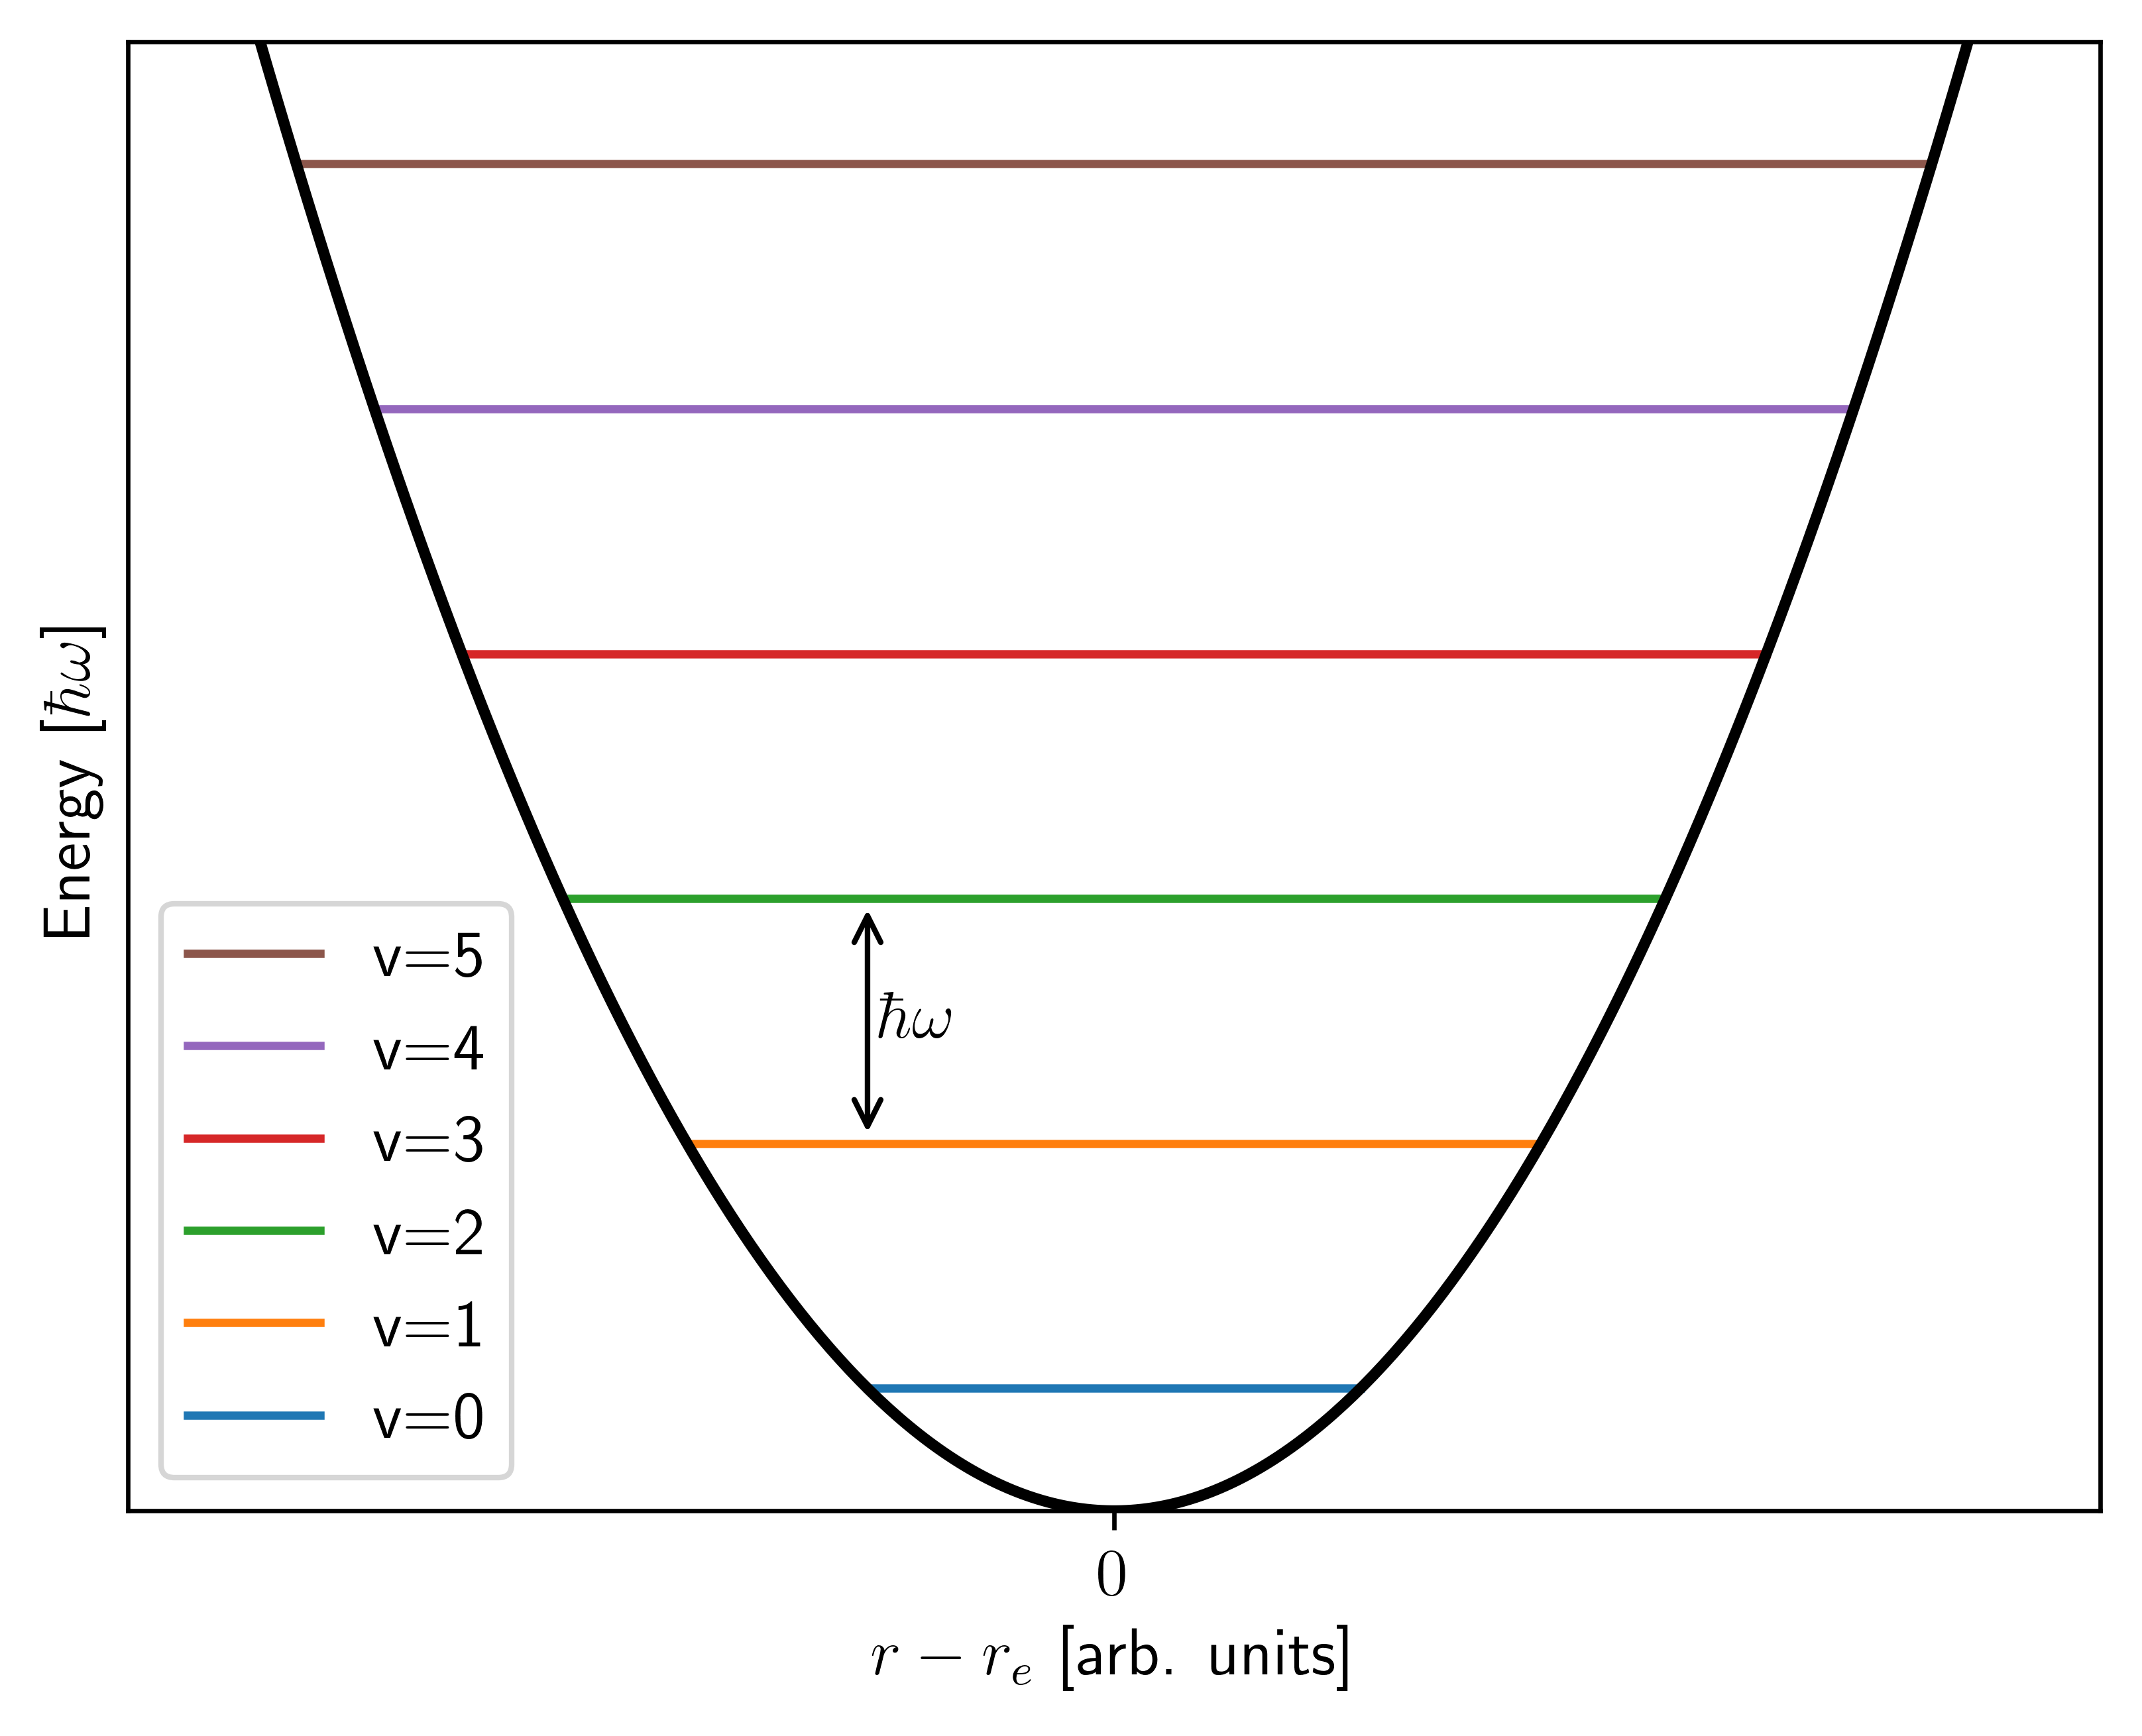
\includegraphics[width=\linewidth]{harmonic_oscillator_energies}
\end{wrapfigure}
The figure to the left shows the first few allowed energy levels of a harmonic oscillator, plotted with the potential shaded in orange. Comparing this to the equivalent plot for a particle in a box (see the previous chapter), there are some critical differences. Firstly, we are allowed to have an energy level at $v=0$, and this is now our \textbf{zero-point energy}, which has an energy of $E_0 = \frac{1}{2}\hbar\omega$. Secondly, the spacing between two adjacent levels is now $\Delta E_v = \hbar\omega$ - that is, it is \emph{constant} (prove it yourself!). For a particle in a box, the spacing increased as $n$ increased - here the spacing is constant. This set of equally spaced energy levels is sometimes called \textbf{vibrational ladder}. However, there are also some similarities to a particle in a box - you will notice that the energy is still \textbf{quantised}. This arises due to the \emph{boundary conditions} again, but here the boundary conditions are from the harmonic potential rather than from two walls of infinite potential. We can analyse the effect that varying the potential will have on the quantisation.

We have seen that $\Delta E_v = \hbar\omega = \hbar\sqrt{\frac{k_f}{m}}$. Evidently, our energy spacing will increase as we increase $k_f$. This is because the potential for a stiffer (higher $k_f$) spring would be more confining, and we've seen previously that tighter boundaries lead to more `aggressive' quantisation (with larger energy gaps). More interesting is the behaviour when $k_f\rightarrow 0$ (this corresponds to a spring being infinitely weak). Under this limit, $\Delta E_v \rightarrow 0$ as well - which means that there is \textbf{no quantisation if the spring is infinitely weak}. If the spring is infinitely weak, the particle on the end of it is completely \textbf{unconstrained and free} - so the gap between adjacent energy levels is infinitely small, i.e. the particle \textbf{isn't quantised any more!} This is entirely as we expect. The final point to make is in relation to the mass $m$. Clearly for larger masses, the energy spacing will decrease. This makes intuitive sense too - \textbf{heavy, macroscopic objects} (like potatoes) \textbf{are not quantised}, and behave classically.

This is also an interesting point at which to consider the quantum-mechanical nature of the zero-point energy. We know that $E_0 = \frac{1}{2}\hbar\omega = \frac{1}{2}\hbar\sqrt{\frac{k_f}{m}}$. Zero-point energy is a completely quantum phenomenon, as classically objects are allowed to have no energy and be stationary (i.e. they can have zero energy). We can see from the equation above that if our spring was infinitely weak, then our zero-point energy would be actually zero - as expected for a free (non-quantised) particle. We can also see that if our mass was infinitely large (and the mass of one of our potatoes is basically infinitely large compared to something like an atom), then our zero point energy would be zero as well. If I stuck a potato on the end of a spring, it could just hang there in a stationary position with zero energy. Quantum mechanically this can't happen. 

\subsection{The Vibrational Wavefunctions}
Having seen the allowed vibrational energies, we can now turn to the allowed vibrational wavefunctions, $\wf_v(x)$. They are given by the equation below:
\begin{equation}
	\wf_v(x) = N_vH_v(\alpha x)\exp{\bigg(-\frac{(\alpha x)^2}{2}\bigg)}, \,\text{where:} \qquad \alpha = \bigg(\frac{mk_f}{\hbar^2}\bigg)^{\frac{1}{4}}
\end{equation}
This looks a bit horrendous, but let's break it down. $N_v$ is simply the normalisation constant associated with the $v$-th vibrational energy level. $H_v(\alpha x)$ is something called a \emph{Hermite Polynomial}, which appears because the differential equation you would end up solving is a form of the \emph{Hermite Equation} - we don't need to get hung up on this, just be aware of what it is (we will meet them again in the context of \textbf{selection rules}). $\alpha$ is a parameter defined above, and you may notice that the final exponential bit is simply a \textbf{Gaussian Function}.

\begin{wrapfigure}{r}{0.55\textwidth}
	\centering
	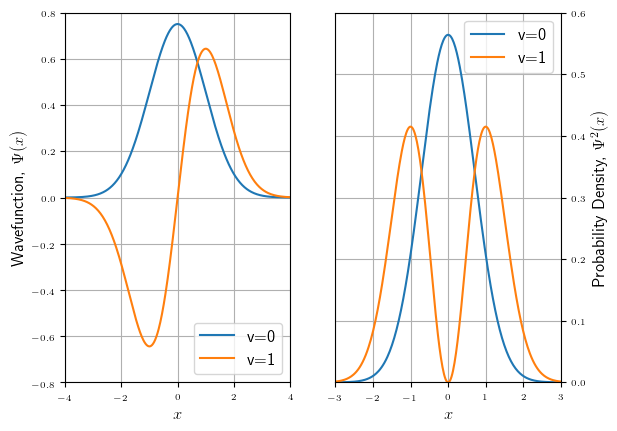
\includegraphics[width=\linewidth]{harmonic_oscillator_wf}
\end{wrapfigure}
The first two wavefunctions for a harmonic oscillator are shown in the leftmost plot in the adjacent figure. The corresponding probability densities are shown in the rightmost plot. The most obvious change as we increment the quantum number $v$ is that at $v=1$ the wavefunction passes through zero - this is a \textbf{node}. We can see this as a point at which there is no probability of finding the particle in the probability density plot. You probably think that these wavefunctions look quite similar to the particle in a box wavefunctions, and you're right! They do look quite similar, even though the mathematical functions are more complicated. We can also see that the wavefunction at $v=0$ now looks a bit like what we might expect classically. A classical harmonic oscillator with zero energy ($v=0$), would be stationary at $x=0$, as the particle wouldn't be oscillating. Here we can see that the \emph{most likely} position for a particle with $v=0$ is at \emph{around} $x=0$, but not \emph{exactly at} $x=0$. This uncertainty in the position arises because the energy isn't zero at $v=0$ (remember the ZPE is $\frac{1}{2}\hbar\omega$). You could imagine that this means the particle is oscillating a little bit around the bottom of the well at $v=0$, so it's not going to be found at \emph{exactly} zero, but will be \emph{somewhere around} zero.

To cement this, let us now consider how we would expect a classical oscillator, like a pendulum, to behave at high energies (when it's actually swinging and isn't stationary). We use a pendulum rather than a spring here as it's easier to visualise, but the behaviour is the same in both cases. As a pendulum swings from side to side, the area where it travels the fastest is as it goes through $x=0$. At the edges of the swing, it's velocity changes direction and so the pendulum is briefly stationary. As such, a moving classical oscillator spends \emph{more time at the edges of it's swing than in the middle}. That is, we would expect to find our particle more often than not \emph{at the edges of it's motion}. Recalling the \textbf{quantum-classical correspondence principle}, we would expect that the behaviour of a quantum oscillator \emph{at high quantum numbers} mirrors the expected classical behaviour. The figure below shows what happens as we increase $v$. 
\begin{figure}[h]
	\centering
	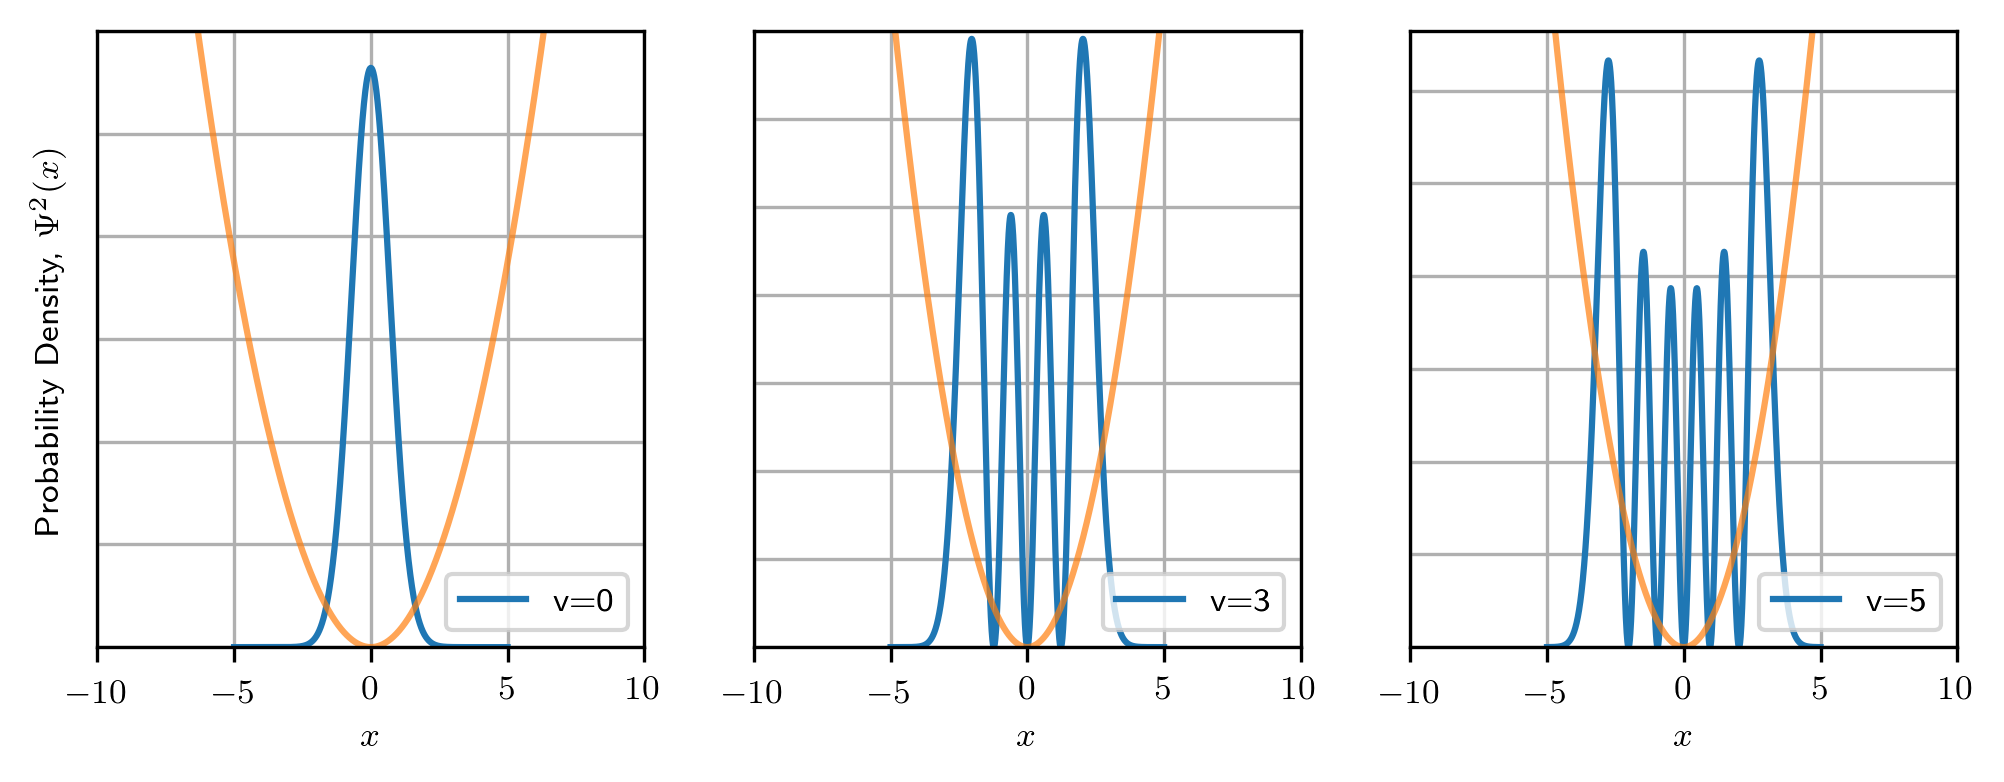
\includegraphics[width=\textwidth]{harmonic_oscillator_probabilities}
\end{figure}
Clearly, as we go to higher vibrational quantum numbers, our particle starts to become more likely to exist at the edges of our harmonic well, and less likely to exist at the center of the well. As predicted, this is completely in line with what we expect, as the particle starts to behave more and more classically as $v$ is increased. Nice!

That's more or less it in terms of vibrational motion for now. A question you're probably asking is: `How good is the approximation that molecules behave as harmonic oscillators?'. The answer is that it's actually quite good! We will see how we can apply the equations generated here to molecules in a later chapter.. 

\begin{myblock}{\begin{center}Particle in Harmonic Potential\end{center}}
	\begin{center}
		\begin{align*} & \text{\textbf{Hamiltonian}} \qquad\qquad \hat{H} = -\frac{\hbar^2}{2m}\frac{\dd^2}{\dd x^2} + V(x),\quad  \text{where} \quad V(x) = \frac{1}{2}k_fx^2, \,\text{where}\,k_f\,\text{is a \emph{force constant}} \\
			& \text{\textbf{Schr{\"o}dinger Equation}} \qquad\qquad -\frac{\hbar^2}{2m}\frac{\dd^2\wf_v(x)}{\dd x^2} + \frac{1}{2}k_fx^2\wf_v(x) = E_v \wf_v(x) \\
			& \text{\textbf{Wavefunctions}} \qquad\qquad \wf_v(x) = N_vH_v(\alpha x)\exp{\bigg(-\frac{(\alpha x)^2}{2}\bigg)}, \,\text{where} \,\alpha = \bigg(\frac{mk_f}{\hbar^2}\bigg)^{\frac{1}{4}},\,\text{and}\, v=0,1,2,3...\\
			& \qquad N_v \text{is a \emph{normalisation constant} for the $v$-th wavefunction, and}\, H_v \text{is the $v$-th \emph{Hermite Polynomial}} \\
			& \text{\textbf{Energies}} \qquad\qquad\qquad\qquad\quad E_v = (v+\frac{1}{2})\hbar\omega \quad \text{where} \quad \omega = \sqrt{\frac{k_f}{m}} \quad \text{and} \quad v=0,1,2,3...
	\end{align*}
	\end{center}
\end{myblock}

\section{Chapter 3 Summary}
What I want you to take away from this chapter:
\begin{itemize}
	\item A \textbf{harmonic oscillator} is a system which experiences a \textbf{restoring force proportional to it's displacement from the origin}. Useful examples are a mass on a spring, and a pendulum.
	\item We can construct a \textbf{quantum harmonic oscillator} by making the potential term in our Hamiltonian, $V(x)$, equal to $\frac{1}{2}kx^2$.
	\item Addition of the \textbf{harmonic potential} results in \textbf{quantisation}, much like the addition of the walls for a particle in a box. The quantum number that we use to describe which state we are in is now the \textbf{vibrational quantum number}, $v$.
	\item The spacing of the energy levels in a quantum harmonic oscillator is equal and \textbf{doesn't change as we increase $v$}. This is in contrast to a particle in a box, where the level spacing increases as $n$ increases.
	\item The \textbf{zero point energy} of a harmonic oscillator is given by $\frac{1}{2}\hbar\omega$ and occurs when $v=0$. This is again in contrast to a particle in a box.
\end{itemize}
In the next chapter, we will look at a different kind of motion, \textbf{rotational motion}, and consider two model systems: the \textbf{particle on a ring} and \textbf{particle on a sphere}.

\chapter{Rotational Motion}

\section{Angular Momentum}
\begin{center}
\begin{quote}
	\textit{\textbf{`Angular Momentum - it makes the world go round!'}} 
\end{quote}
\end{center}
You've probably seen the quote above on those terribly unfunny t-shirts that physicists like to wear to compensate for the fact that they have no friends.

It's true, however, in two senses. Firstly the obvious sense in that as the earth spins it has \textbf{angular momentum}. Secondly, it's \emph{absolutely critical} to the behaviour of all atoms and molecules. The universe would not function as we know it without angular momentum! So what is angular momentum?

\textbf{Angular momentum} is probably most easily understood by comparing to a (hopefully) familiar quantity, \textbf{linear momentum}. Linear momentum (given the symbol $p$) is simply the product of the mass of an object and it's velocity, that is: $p = mv$. \textbf{Angular momentum} (given the symbol $J$) can be defined in a completely analogous way, but instead of mass and velocity, we define two new quantities: \textbf{angular velocity} (given the symbol $\omega$) and \textbf{moment of inertia} (given the symbol $I$). We also need to make clear that when we do rotational motion, we are always rotating \emph{around} some central point, called the \textbf{origin}. 

\begin{wrapfigure}{r}{0.4\textwidth}
	\centering
	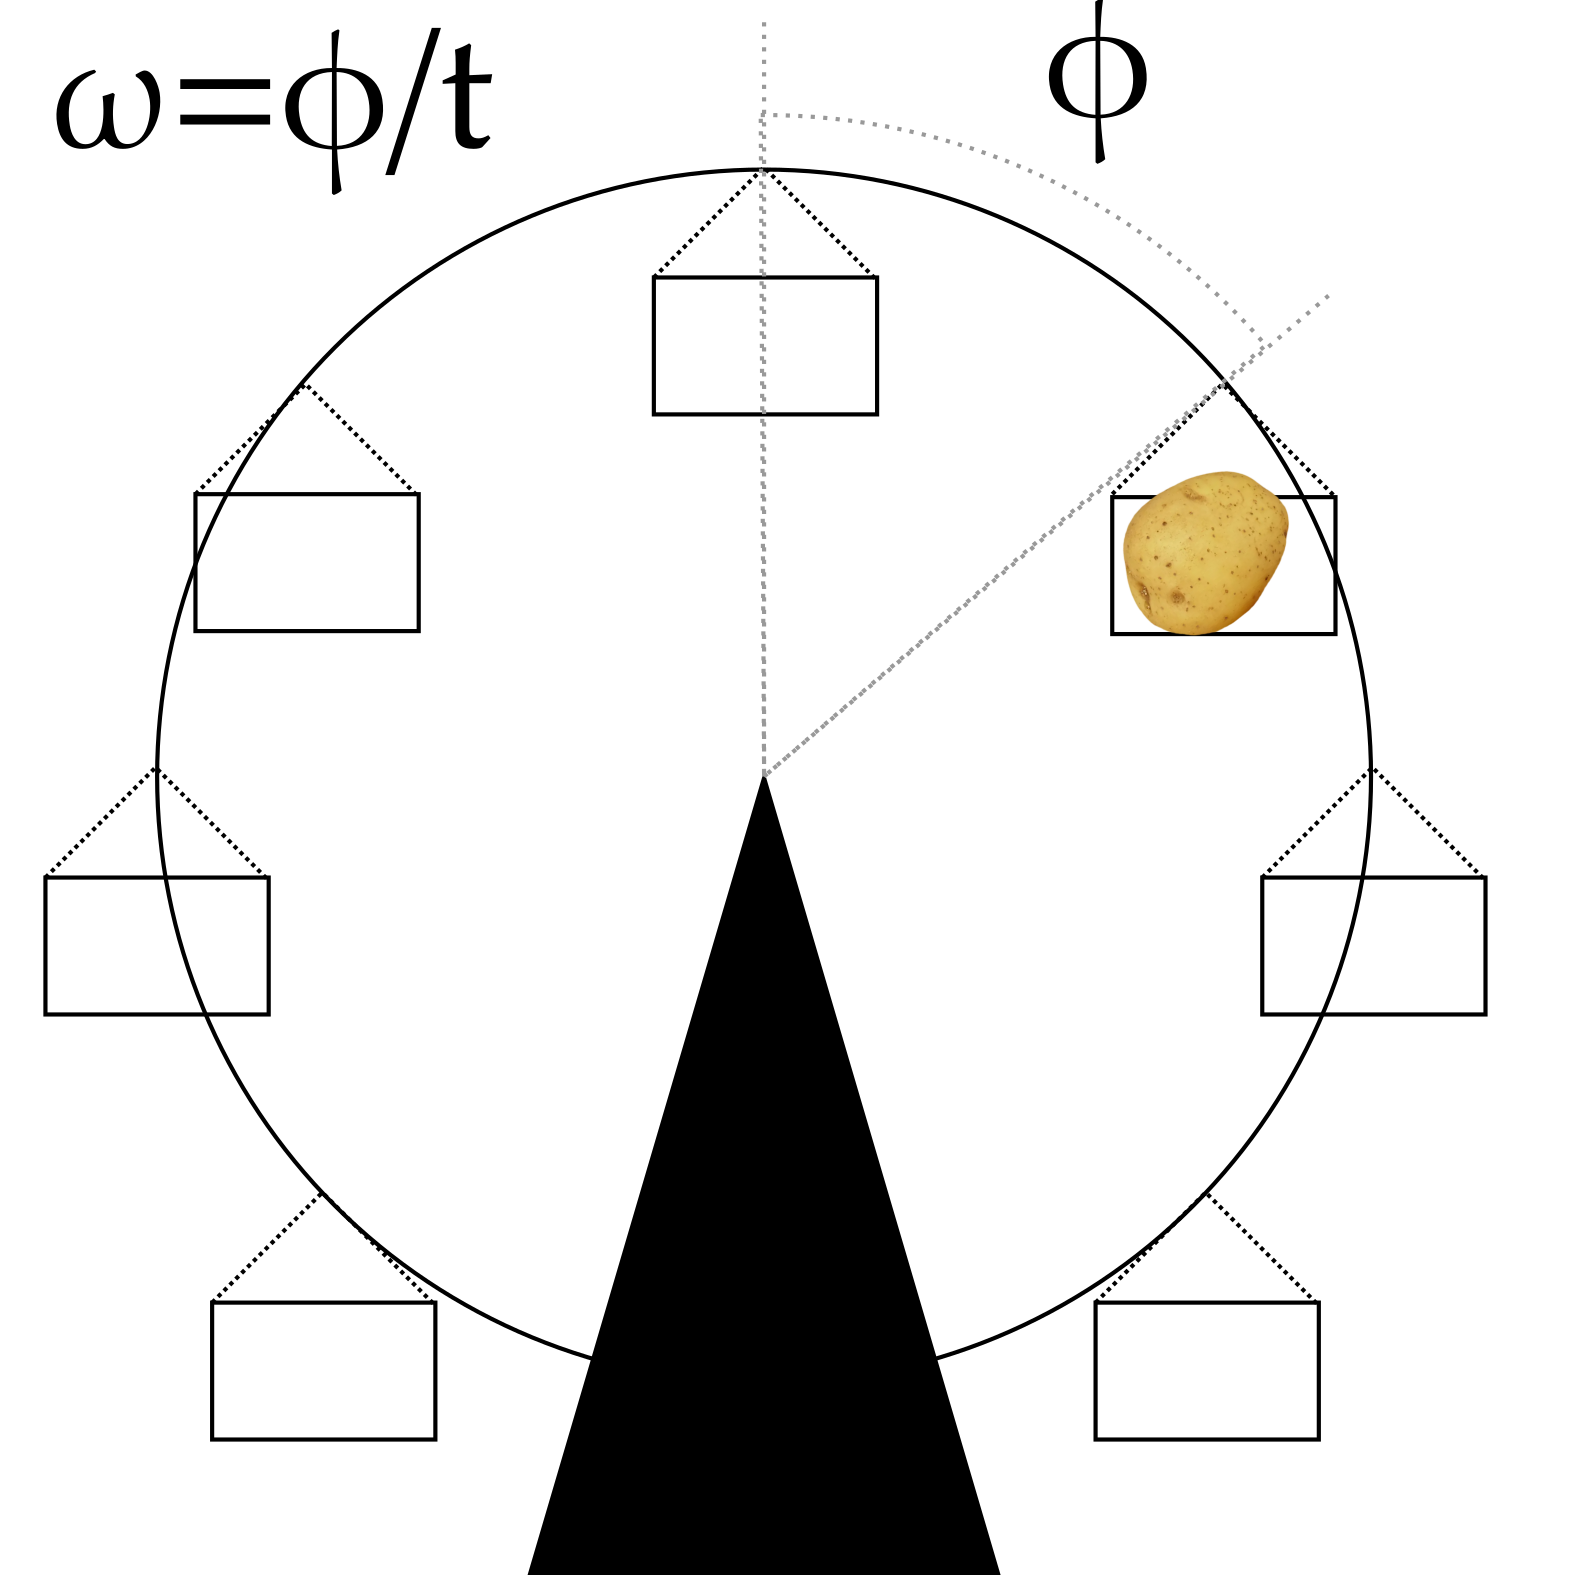
\includegraphics[width=0.9\linewidth]{angular_velocity.png}
\end{wrapfigure}
Whereas linear velocity (or just `velocity') is defined as the \emph{distance travelled per unit time}, the \textbf{angular velocity} is defined as the \emph{angle swept out per unit time}. We will call this angle $\phi$, and it's illustrated on the adjacent figure. Imagine a ferris wheel - I could stand at the bottom, put a potato in one of the carriages, and count how many times in a minute I see the potato fly past me. If the ferris wheel was travelling with a \emph{high angular velocity}, I would see the potato several times a minute. If the ferris wheel was travelling with a \emph{low angular velocity}, I would only see the potato a few times, or maybe only once. The units of \textbf{angular velocity} are \textbf{radians per second}. 

Turning now to \textbf{moment of inertia}, this is sometimes defined as \emph{angular mass}. Mass, as we tend to think about it, is how \emph{heavy} something is. But we're scientists, and so can think of a cleverer and more subtle explanation - mass is the \emph{tendency for an object to resist acceleration}. If an object is very heavy (high mass), it's difficult to push it and make it start moving - it tends to \emph{resist} the acceleration we are trying to apply to it. Moment of inertia, then, is just the angular equivalent of this. Moment of inertia is the \textbf{tendency for an object to resist angular acceleration}. It's difficult to make things with a high moment of inertia start rotating. Mathematically, the moment of inertia $I$ of a system consisting of $N$ different particles is defined as:
\begin{equation}
	I = \sum_{i=1}^N m_ir_i^2
\end{equation}
Where $m_i$ is the mass of particle $i$, and $r_i$ is the perpendicular distance from $i$ to the \emph{axis of rotation} (this could be the distance to a chemical bond, for example). We can imagine that our system of $N$ masses is a molecule consisting of $N$ atoms. Without going into a lot of detail, it's clear that if we have heavier atoms, or atoms that are very far away from what they're rotating around, then it's harder to get the molecule to rotate and the \textbf{moment of inertia} is higher. This should intuitively make sense! 

Returning to our original subject, \textbf{angular momentum}, now we understand the two concepts that make it up, we are in a position to understand it. In the same way that linear momentum = mass $\times$ velocity, angular momentum = moment of inertia $\times$ angular velocity, i.e:
\begin{equation}
	J = I\omega
\end{equation}
So, we can see that the faster something is rotating (higher $\omega$), and the bigger the moment of inertia (higher $I$), then the larger the angular momentum. When we talk about angular momentum, we talk about \emph{angular momentum around a certain rotation axis}. In a chemical setting, we might talk about the \emph{angular momentum around chemical bond}. This will hopefully become clearer in the figures below.

\begin{figure}[h]
	\centering
	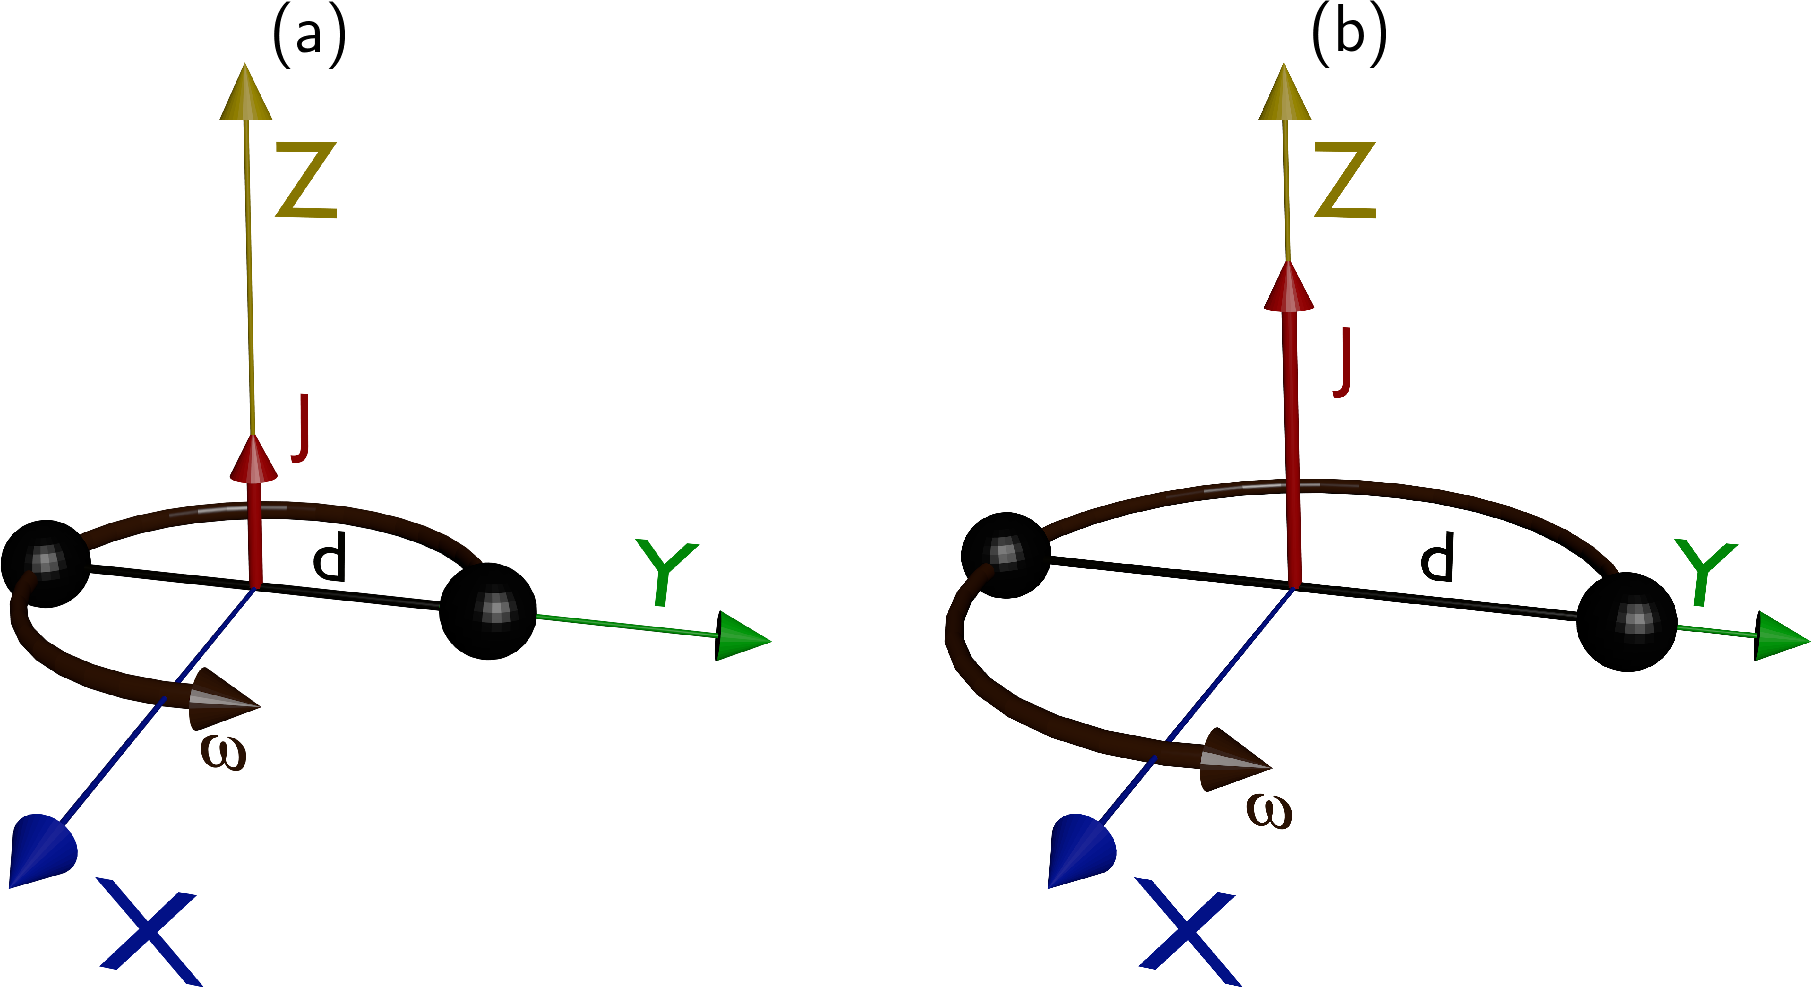
\includegraphics[width=0.9\textwidth]{angular_momenta}
	\caption{A model of a homonuclear diatomic molecule with atoms of mass $m$ and a bond length $d$, rotating freely around the $Z$ axis in the $XY$ plane with an angular velocity $\omega$. The resultant angular momentum around the $Z$ axis is shown in red. The leftmost figure shows that a shorter bond length leads to a smaller angular momentum as the moment of inertia is reduced. The rightmost figure shows that a longer bond length leads to a larger angular momentum due to the larger moment of inertia.}\label{fig:angular_momenta}
\end{figure}
It will be useful to be aware of that, like linear momentum, angular momentum is a \emph{vector quantity}. That is, it has both a \emph{direction} and a \emph{magnitude}\footnote{In contrast, mass or moment of inertia are \emph{scalar quantities}, they only possess a magnitude and not a direction. Angular and linear velocity are both \emph{vector quantities} too, but \emph{speed} is a scalar quantity}. It's not immediately clear what the `direction' of the angular momentum vector is. In the linear case, the direction of the momentum vector is the same as that of the velocity vector ($p=mv$). We said that when we discuss angular momentum, we discuss the angular momentum \emph{around a certain rotation axis}. So, an obvious way to represent the angular momentum vector is as a vector \emph{directed along the rotation axis, where the length of the vector shows the magnitude of the angular momentum}. This is shown graphically in the image below, for two diatomic molecules (each with different bond lengths) rotating in the $xy$ plane, around the $z$ axis. Clearly, the molecule with the larger bond length (b) will have a larger moment of inertia than (a), so the angular momentum, $J$, is correspondingly larger. 

\begin{table}[]
\centering
\begin{tabular}{@{}lll@{}}
\toprule
Quantity & Linear Motion & Angular Motion \\ \midrule
Resistance to Acceleration & Mass, $m$ & Moment of Inertia, $I$  \\
Velocity  & \bv = $\frac{d}{t}$ & \bw = $\frac{\phi}{t}$ \\
Momentum & \bp = m\bv & \bj = I\bw \\
Kinetic Energy (in terms of velocity) & $E_{\text{Tr.}} = \frac{1}{2}m\bv^2$ & $E_{\text{Rot.}} = \frac{1}{2}I\bw^2$  \\
Kinetic Energy (in terms of momentum) & $E_{\text{Tr.}} = \frac{\bp^2}{2m}$ & $E_{\text{Rot.}} = \frac{\bj^2}{2I}$ \\ \bottomrule
\end{tabular}
	\caption{Physical quantities and how they are defined for linear and angular motion.}\label{tab:lin_ang}
\end{table}


\section{Quantum Mechanical Rotation}
Having gained an understanding of the classical differences between translational (linear) and rotational motion, we will now tackle the same problem quantum mechanically. We will find that this is quite a satisfying problem, if we have understood the previous few chapters. Firstly, we will look at the simplest possible case, rotational motion in two dimensions (the `Particle on a Ring' system). Following this, we will extend the analysis to rotational motion in three dimensions (`Particle on a Sphere'), and see how this changes things - ending up with some familiar (hopefully) expressions from rotational spectroscopy. 

Before we do this, it is useful to quickly discuss the nomenclature surrounding \textbf{angular momentum}. So far, we have used the symbol $J$. We will use this when we talk about classical angular momentum, or when we talk about the \emph{total angular momentum} of molecules in Chapter 6. When we talk about the model systems below, we will use the symbol $l$. The reason for this is that in the model systems, we are \textbf{specifically talking about orbital angular momentum} - the angular momentum a particle has as it spins around something. This has the symbol $l$. If we were talking about molecules, they might also have \textbf{spin angular momentum}, so we have to use the symbol $J$ because that includes the possibility of \textbf{spin}. 

Just remember: classical or molecules = $J$. Model systems here = $l$.
\subsection{A Particle on a Ring}
\begin{wrapfigure}{l}{0.3\textwidth}
	\centering
	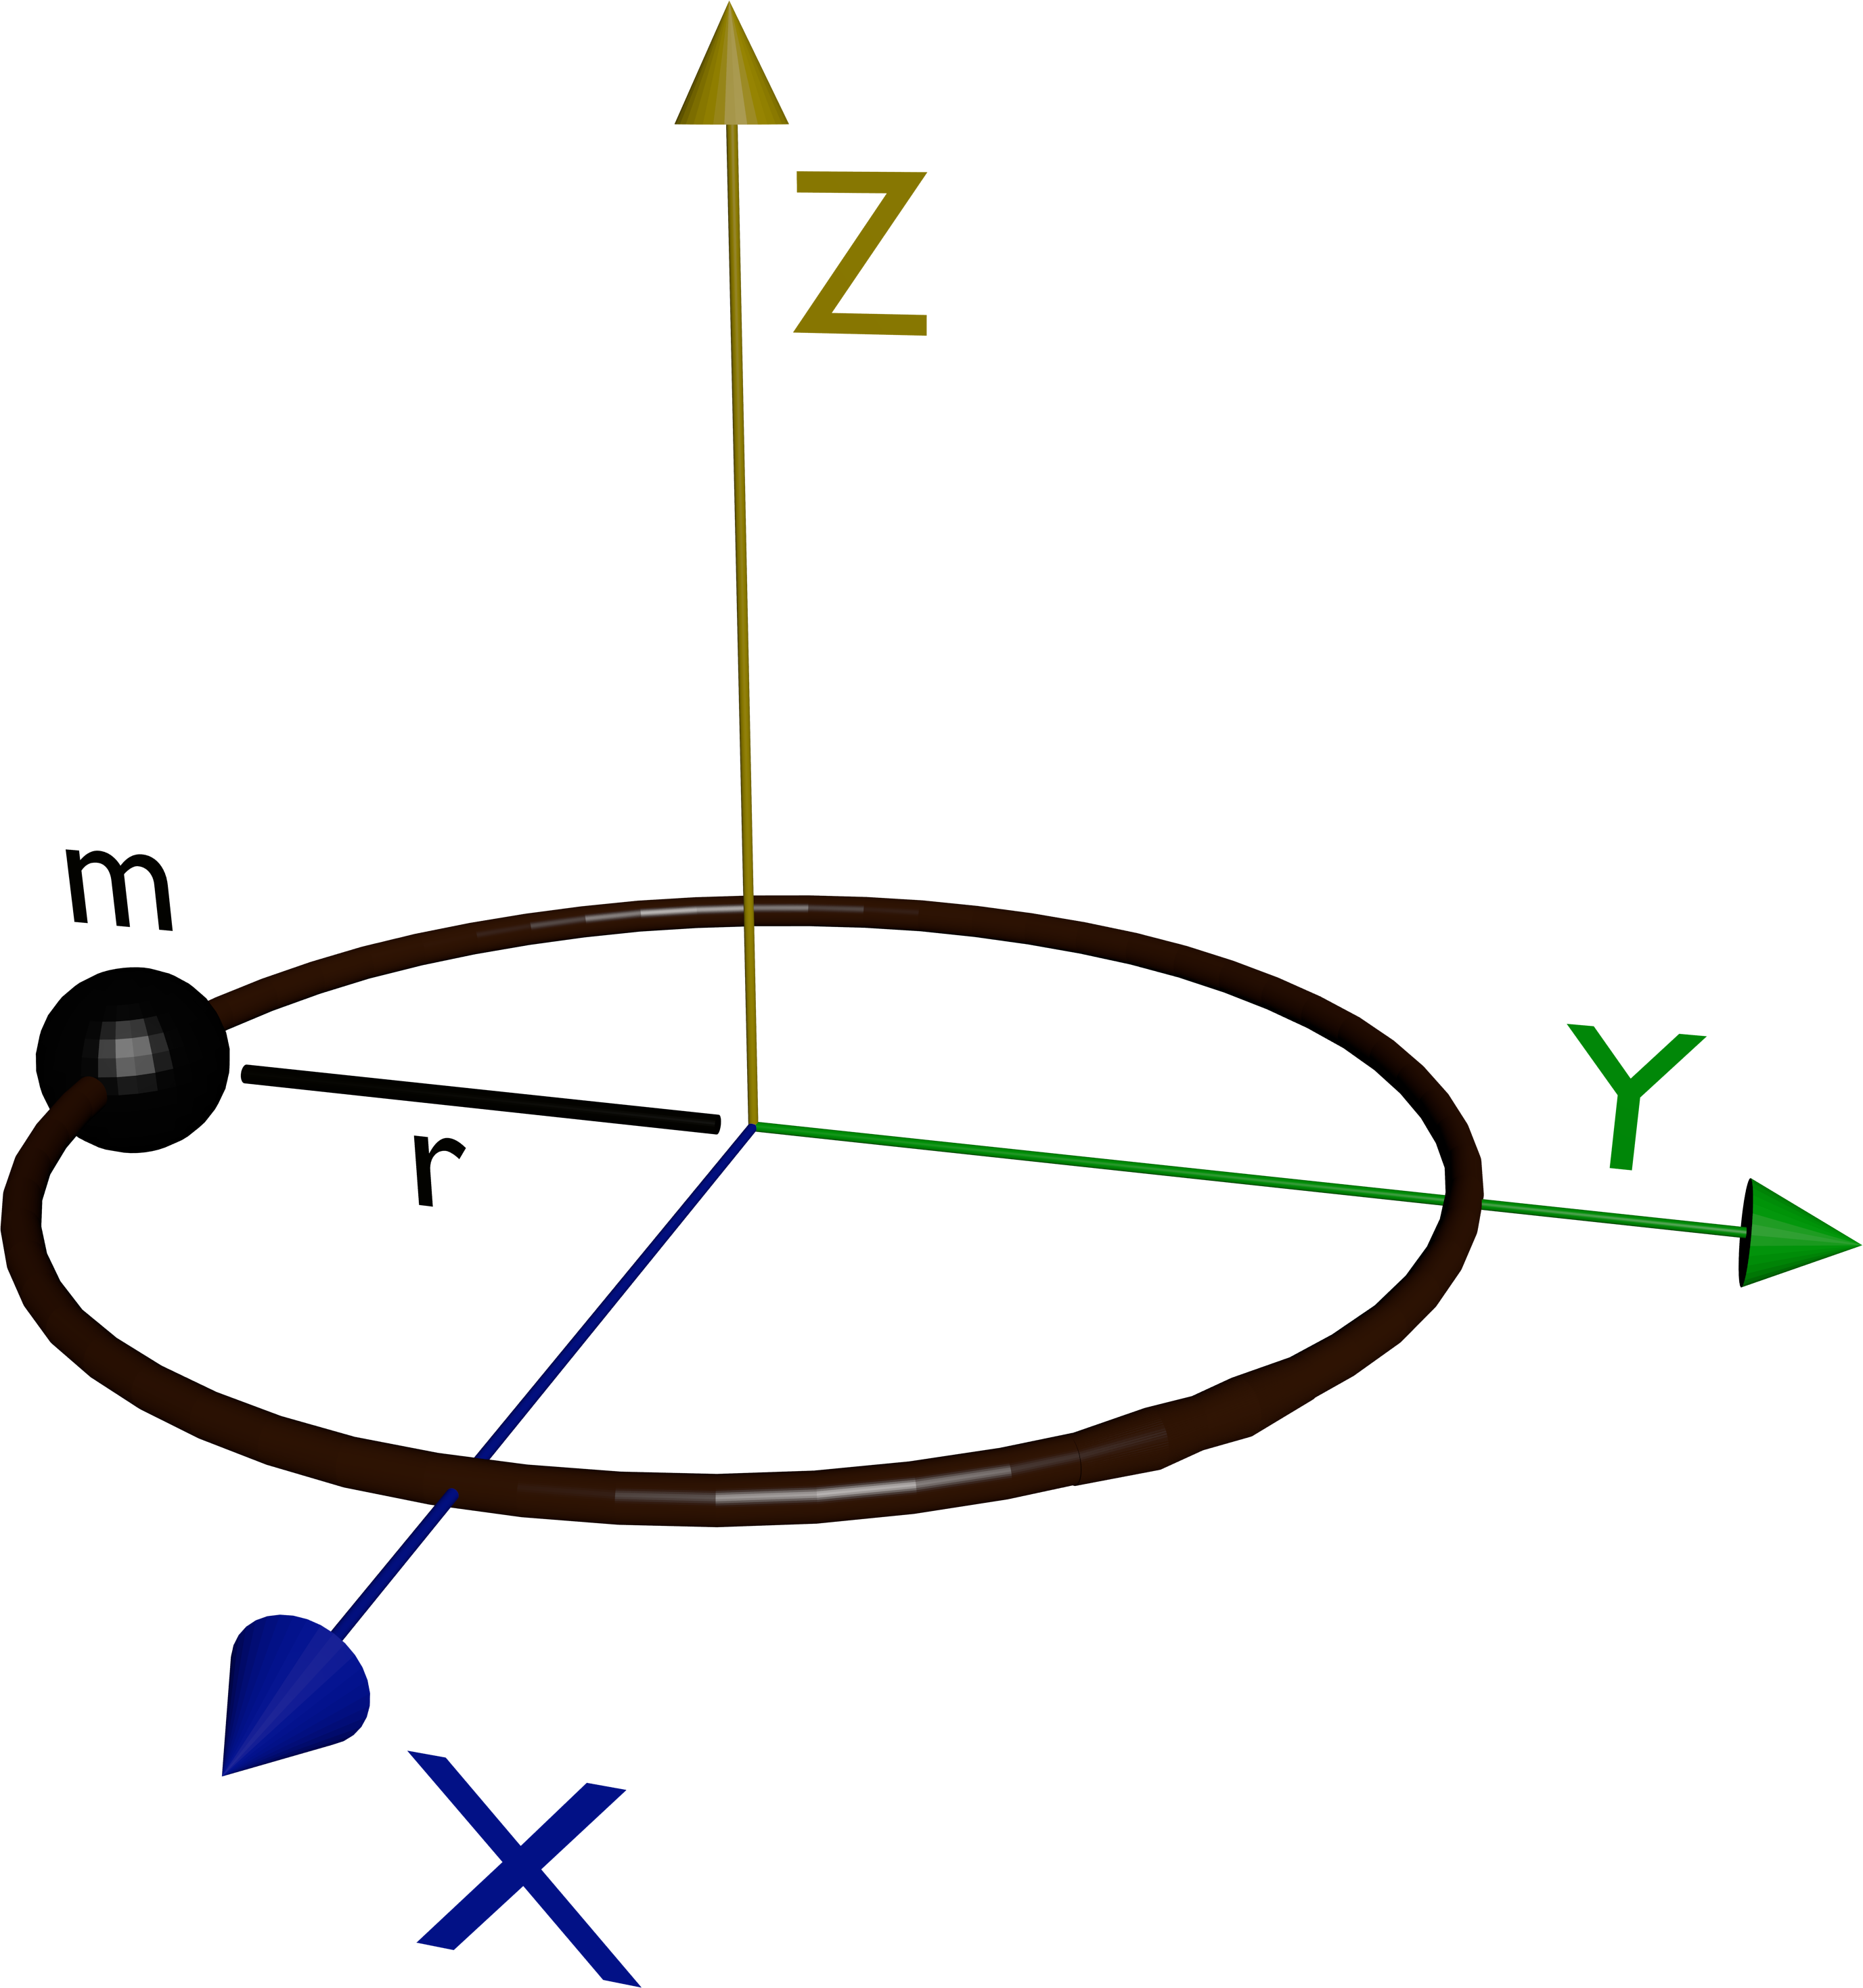
\includegraphics[width=\linewidth]{particle_on_a_ring}
\end{wrapfigure}
Imagine a particle of mass $m$ placed on a ring with a radius $r$. By convention, the ring lies in the $xy$ plane, such that the particle rotates around the $z$ axis. The particle is free to rotate around the ring. This situation is illustrated in the adjacent figure.

\subsubsection{The Schr{\"o}dinger Equation}
The first thing we need to do is figure out what our Hamiltonian is. We know that the Hamiltonian expresses the \emph{total energy of the system}, and that this is the sum of the kinetic and potential energies. We said that the particle is free to rotate around the ring, so the potential energy is zero (as rotation is free). However, the kinetic energy will be non-zero. 

We know from the previous chapters that for a particle of mass $m$ that is free to move in one dimension \textbf{linearly} (along $x$), the Hamiltonian consists of a kinetic energy term and is given by:
\begin{equation}\label{eq:hamiltonian_linear}
	\hat{H} = -\frac{\hbar^2}{2m}\frac{\dd^2}{\dd x^2}
\end{equation}
This equation is just the Hamiltonian we used for our particle free to move in one dimension in chapter 2. So what is the equivalent of this for a particle that is free to rotate around a ring? The answer is deceptively simple, and can be obtained just by comparison with the Hamiltonian above. We know from~\autoref{tab:lin_ang} that the equivalent of mass for rotational motion is the \emph{moment of inertia} $I$, so the first thing we should do is replace $m$ with $I$. The other thing to change is the derivative term, as now we are not just moving along $x$, but are rotating \emph{in the $xy$ plane, by some angle $\phi$}. If we restrict ourselves to a ring that cannot change in size (i.e. a ring for which the radius is \emph{fixed}), then the only motion we can do is around the ring, which we can describe using the angle $\phi$. So replacing $x$ with $\phi$, we can write our Hamiltonian as:
\begin{equation}\label{eq:hamiltonian_rotation}
	\hat{H} = -\frac{\hbar^2}{2I}\frac{\dd^2}{\dd \phi^2}
\end{equation}
If you're interested (I am), this Hamiltonian can also easily be derived by starting with~\autoref{eq:hamiltonian_linear}, but extending it to free motion in the $xy$ plane:
\begin{equation}
	\hat{H} = -\frac{\hbar^2}{2m}\bigg(\frac{\dd^2}{\dd x^2} + \frac{\dd^2}{\dd y^2}\bigg)
\end{equation}
Changing the coordinate system from Cartesian to Polar (remember $x = r\cos\phi$ and $y = r\sin\phi$), and restricting ourselves to a ring of a fixed radius, allows~\autoref{eq:hamiltonian_rotation} to be derived easily. Give it a shot!

With the Hamiltonian given in \autoref{eq:hamiltonian_rotation}, we can now write our SE for a particle on a ring (note I have added the subscript "R" to denote that these are rotational energies and wavefunctions).
\begin{equation}
	\hat{H}_{\text{R}} \wf_{\text{R}} = E_{\text{R}} \wf_{\text{R}}
\end{equation}
\begin{equation}
	-\frac{\hbar^2}{2I}\frac{\dd \wf_{\text{R}}}{\dd\phi^2} = E_{\text{R}} \wf_{\text{R}}
\end{equation}
Where $E_{\text{R}}$ is the rotational energy. This can be simply rewritten as: 
\begin{equation}
	\frac{\dd \wf_{\text{R}}}{\dd\phi^2} = -\frac{2IE_{\text{R}}}{\hbar^2}\wf_{\text{R}}
\end{equation}
The general solution to this equation is given by:
\begin{equation}\label{eq:rotational_general_solution}
	\wf_{\text{Rot.}} = \frac{1}{\sqrt{2\pi}}\mathrm{e}^{im_l\phi}\,\quad\text{where}\quad\,m_l=\sqrt{\frac{2IE_{\text{Rot.}}}{\hbar^2}}
\end{equation}
Here $m_l$ is a another \textbf{quantum number}, which we will analyse in more detail shortly. Try and verify that the solution I've presented is actually a solution!

A simple rearrangement of the above expression for $m_l$ yields an expression for the rotational kinetic energy $E_{\text{Rot.}}$:
\begin{equation}
	E_{\text{Rot.}} = \frac{(m_l \hbar)^2}{2I}
\end{equation}
Compare this to the expression for the translational kinetic energy in \autoref{eq:pinbox_general}, reproduced below.
\begin{equation*}
	E_{\text{Kin.}} = \frac{(k\hbar)^2}{2m} \tag{\ref{eq:pinbox_general}}
\end{equation*}
We can see that they're very similar expressions! The only differences are that we have a different quantum number, $m_l$, not $k$, and we now use the \emph{moment of inertia} rather than the \emph{mass}. Looking back at the different ways we can express translational and rotational kinetic energy in the table from the first section, it is clear that where in\autoref{eq:pinbox_general} we could identify $k\hbar$ as giving us linear momentum (along $x$ in that case), here $m_l\hbar$ must give us the \textbf{angular momentum along $z$} in units of $\hbar$. This was illustrated in~\autoref{fig:angular_momenta}, the only difference is that there we called the angular momentum $J$, whereas here we refer to it as $m_l$ for reasons that will become clear later.   

Furthermore, we so far haven't seen any constraints on the value of $m_l$ - this means that at the moment our particle can have any angular momentum it wants, and therefore any energy that it wants. $m_l$ can even be positive or negative - just like $k$ could be positive or negative in \autoref{eq:pinbox_general}. In the translational case, different signs of $k$ represented momentum in opposite directions - here, different signs of $m_l$ correspond to different directions of \textbf{rotation around the ring}. This is illustrated below. 
\begin{figure}[h]
	\centering
	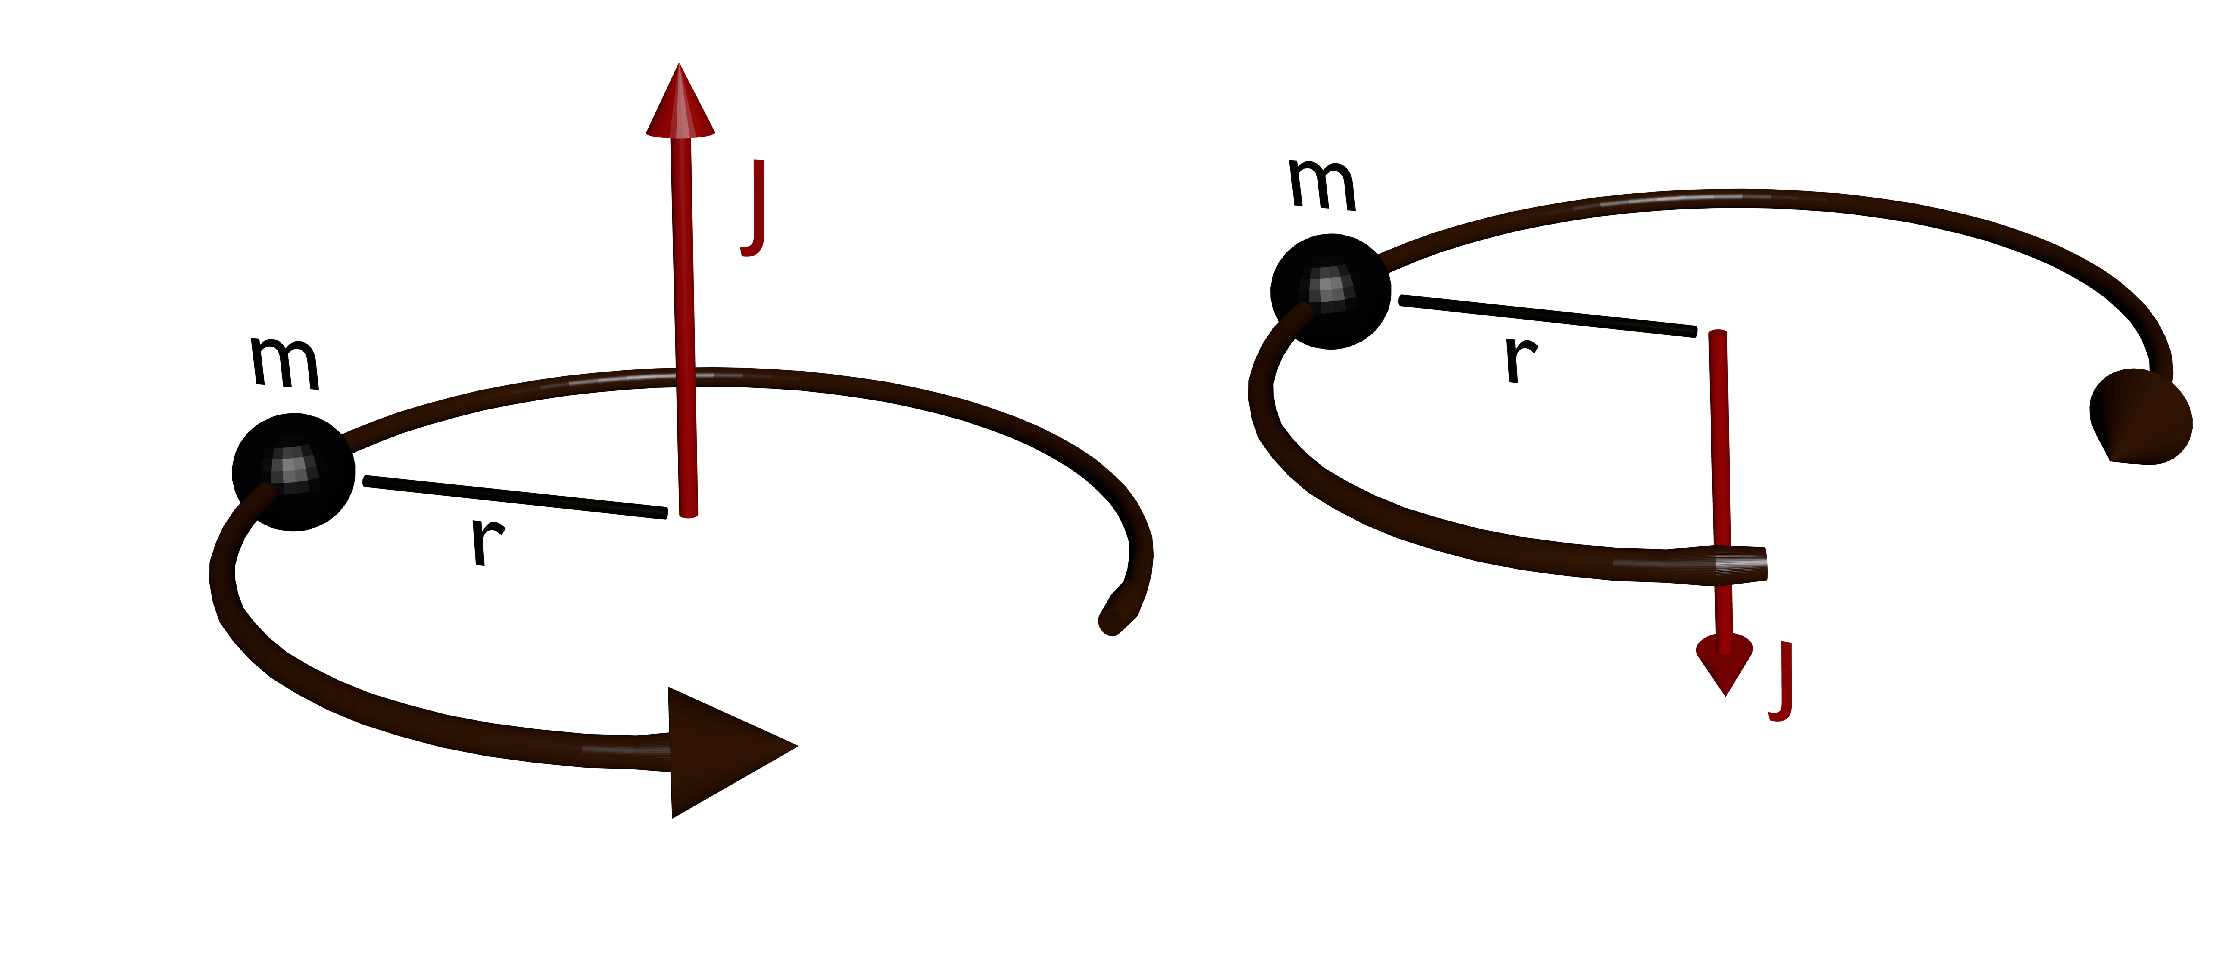
\includegraphics[width=0.6\textwidth]{angular_momentum_directions}
	\caption{Different directions of rotation around the ring correspond to different signs of $m_l$. By convention, anti-clockwise rotation gives a positive value of $m_l$, and clockwise rotation gives a negative value.}
\end{figure}

Continuing this quite pleasant comparison to the translational case, we saw then that the \textbf{quantisation of energy occurred when boundary conditions were imposed}. The same will be true here - so what are the \emph{rotational boundary conditions?}

\subsubsection{The Boundary Conditions and Quantisation}
Recall from the first chapter the characteristics of acceptable wavefunctions - they must be \textbf{continuous, single valued}, and \textbf{cannot be zero everywhere or infinite everywhere}. Our job here is a bit different from the particle in a box case, as we don't have areas of infinite potential to contend with. In that case, the trouble was making our wavefunction go smoothly to zero at the edges of the box - it was hard to make the wavefunction \textbf{continuous}. Here, we don't have this problem, but we do have a problem in making our wavefunction \textbf{single-valued}. 

What do I mean by this? Well, the ring is a circle, obviously. This might not be a particularly astounding observation, but it has important impacts for the quantum mechanics. If I have a wavefunction that depends on some angle $\phi$, it's going to overlap itself everytime it makes a complete revolution of the ring (i.e. every time that it rotates by an angle of $2\pi$ radians). This is important - because my wavefunction needs to be \textbf{single-valued}, the value of the wavefunction at $\phi$ \textbf{must be the same as} the value of the wavefunction at $\phi+2\pi$. If this wasn't the case, then my wavefunction could have two values at the same $\phi$ - which is not allowed! Have a look at the image below showing two rings with two potential wavefunctions. The wavefunction on the left (in blue) is acceptable - this wavefunction is smooth and continuous and is \textbf{single valued}. Conversely, the wavefunction on the right (in red) is unacceptable - look at the area marked with the orange dashed line. In this area, the wavefunction has two values, one part of it is above the ring, but this overlaps another part below the ring! Clearly this wavefunction is \textbf{not acceptable}. 
\begin{figure}[h]
	\centering
	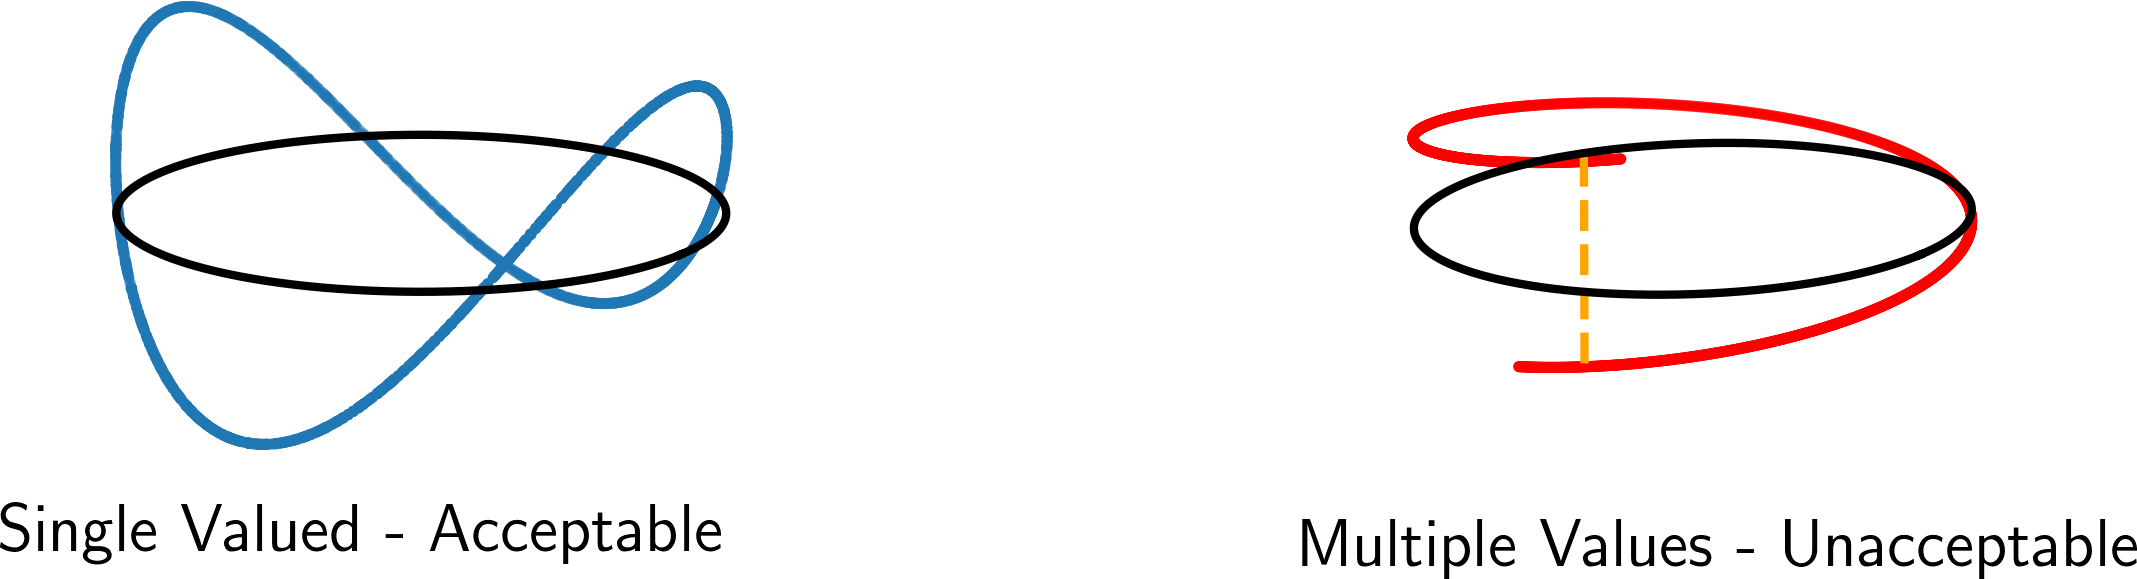
\includegraphics[width=\textwidth]{rotational_wavefunctions}
	\caption{Two possible wavefunctions for a particle on a ring. The leftmost wavefunction is acceptable. The rightmost wavefunction is not, as it has multiple values in the area indicated by the orange line.}
\end{figure}

Mathematically, this boundary condition can be expressed as the aptly named \textbf{cyclic boundary condition}:
\begin{equation}
	\wf_{\text{Rot.}}(\phi) = \wf_{\text{Rot.}}(\phi + 2\pi)
\end{equation}
Which simply states the the value of the wavefunction somewhere on the ring, at $\phi$, has to be the same as the value of the wavefunction when we've travelled 360 degrees ($2\pi$ radians) around the ring - one complete revolution. If you substitute the equation for $\wf_{\text{Rot.}}$ from~\autoref{eq:rotational_general_solution} into the above equation, then you are able to show that the \textbf{only acceptable wavefunctions exist when $m_l$ is an integer}. This is outlined below:
\begin{equation}
	\wf_{\text{Rot.}}(\phi) = \frac{1}{\sqrt{2\pi}}\mathrm{e}^{im_l\phi} = \wf_{\text{Rot.}}(\phi+2\pi) = \frac{1}{\sqrt{2\pi}}\mathrm{e}^{im_l(\phi+2\pi)}
\end{equation}
Cancelling out some constants and remembering the rules of exponents, we can then write:
\begin{equation}
	\mathrm{e}^{im_l\phi} = \mathrm{e}^{im_l\phi}\mathrm{e}^{2\pi m_li}
\end{equation}
Which lets us then cancel out the $\mathrm{e}^{im_l\phi}$ parts and write:
\begin{equation}
	\mathrm{e}^{2\pi m_li} = 1
\end{equation}
This is where we need to be clever. As well as the SE, also on our list of `Most Important Equations of All Time' would probably be \emph{Euler's Formula}, which states.
\begin{equation}
	\mathrm{e}^{i\pi} = -1
\end{equation}
Therefore, we can write our overall \textbf{boundary condition} as:
\begin{equation}
	\wf_{\text{Rot.}}(\phi+2\pi) = (-1)^{2m_l}\wf_{\text{Rot.}}(\phi)
\end{equation}
Which means, that for an \emph{acceptable wavefunction}, we require that:
\begin{equation}
	(-1)^{2m_l} = 1
\end{equation}
This mean that $2m_l$ must be a \textbf{positive or negative even number}, which means that $m_l$ \textbf{must be a positive or negative integer}. So now we have quantisation of our particle on a ring! $m_l$ can be positive or negative as we can rotate in either direction around the ring. Note that the expression for the energy depends on $m_l^2$, so that a negative value of $m_l$ doesn't give us a negative energy! We can now write the full solution below as follows.  

\begin{myblock}{\begin{center}Particle on a Ring\end{center}}
	\begin{center}
		\begin{align*} & \text{\textbf{Hamiltonian}} \qquad\qquad \hat{H} = -\frac{\hbar^2}{2I}\frac{\dd^2}{\dd \phi^2} \,\quad  \text{where} \quad I \,\,\text{is the \emph{moment of inertia}} \\
			& \text{\textbf{Schr{\"o}dinger Equation}} \qquad\qquad -\frac{\hbar^2}{2I}\frac{\dd^2\wf_R(\phi)}{\dd \phi^2} = E_R \wf_R(\phi) \\
			& \text{\textbf{Wavefunctions}} \qquad\qquad \wf_R(\phi) = \frac{1}{\sqrt{2\pi}}\mathrm{e}^{im_l\phi} \quad \text{where} \quad m_l=0,\pm1,\pm2,\pm3...\\
			& \text{\textbf{Energies}} \qquad\qquad\qquad\qquad\quad E_R = \frac{(m_l\hbar)^2}{2I} \quad \text{where} \quad m_l=0,\pm1,\pm2,\pm3...
	\end{align*}
	\end{center}
\end{myblock}

This hopefully all makes sense. We've seen that it's possible to have \textbf{quantised rotation}, and that the quantum number $m_l$ tells us about the size of the \textbf{angular momentum along the rotation ($z$) axis}. We will now move on to a more complex problem - the \textbf{particle on a sphere}.
\newpage
\section{The Particle on a Sphere}
Now we will tackle a more complex problem, where we imagine that our particle is confined to the \emph{surface of a sphere}. The motion of the particle on the surface is still unconstrained (so we have no potential energy terms to worry about), but now we have an extra dimension that we can move in. Not only can we rotate around the equator of the sphere (like a ring), but we can also move up and down the sphere. This means we now have two angles that we're working with, $\theta$ and $\phi$, rather than just $\phi$ (as we were previously). These angles are illustrated on the adjacent figure. 
\begin{wrapfigure}{r}{0.3\textwidth}
	\centering
	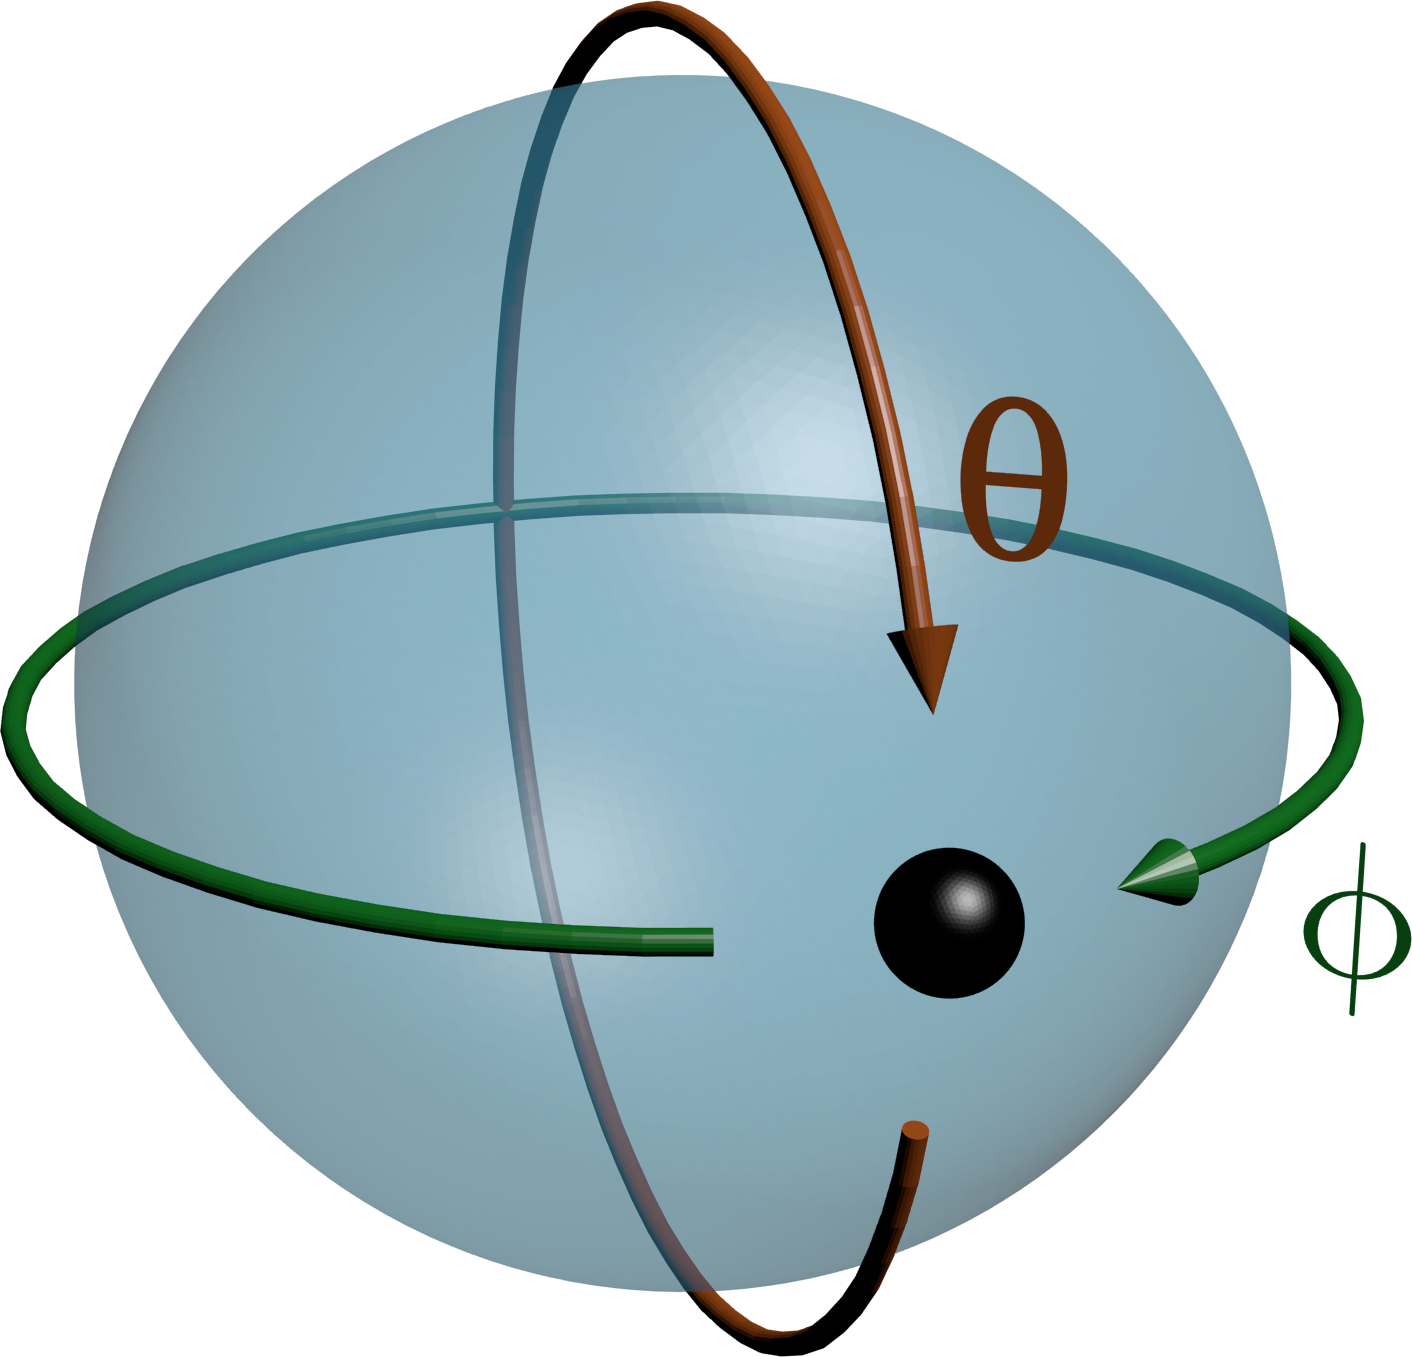
\includegraphics[width=\linewidth]{particle_on_sphere}
\end{wrapfigure}

The next obvious thing to do is think about what our Hamiltonian is. In the previous case, we simply constructed it by comparison with an equivalent Hamiltonian for linear motion. This is \textbf{not} possible here unfortunately, as the move from two dimensional (confined to $xy$) motion to three dimensional motion adds a lot more complexity. However, this is still an interesting place to start, so the Hamiltonian for unrestricted motion in three dimensions, for a particle with mass $m$, is given by:
\begin{equation}\label{eq:hamiltonian_3d}
	\hat{H} = \frac{\hbar^2}{2m}\bigg(\frac{\dd^2}{\dd x^2} + \frac{\dd^2}{\dd y^2} + \frac{\dd^2}{\dd z^2}\bigg)
\end{equation}
If we were masochists, we could convert our coordinate system from Cartesian to Spherical, and derive an expression in terms of $r, \theta$ and $\phi$. However, there's chemistry to do and molecules to think about, so we don't have time for this. 

What we will do instead imagine that we have done this and write our Hamiltonian using a new function called $\nabla^2$ (which is pronounced ``del squared'' and has the fancy french name ``The Laplacian''). This new function consists of a part that calculates the radial motion (i.e. motion from the center of the sphere outwards), and a part that calculates the \emph{angular motion} - i.e. the motion \emph{over the surface of the sphere}. Think of $\nabla^2$ as just combining all of the derivative terms in~\autoref{eq:hamiltonian_3d}, but in spherical coordinates, so we could write:
\begin{equation}
	\hat{H} = \frac{\hbar^2}{2I}\nabla^2
\end{equation}
Where we have swapped our $m$ for $I$ as now we are explicitly talking about rotations. We will assume that our radius is fixed and that our particle can only move over the surface of the sphere. This means that we can ignore the radial part of $\nabla^2$ and focus on the angular part.  

Unfortunately, the angular part is still \textbf{horrifically complicated} if we wanted to actually solve it here and now. The angular part also has a fancy french name (``The Legendrian''), and has the symbol $\Lambda^2$. It is given by (bear with me!):
\begin{equation}
	\Lambda^2 = \frac{1}{\sin^2\theta}\frac{\dd^2}{\dd\phi^2} + \frac{1}{\sin\theta}\frac{\dd}{\dd \theta}\sin\theta\frac{\dd}{\dd\theta}
\end{equation}
See? Pretty horrible. However it does mean that we can write our Hamiltonian for the particle on a sphere (assuming a fixed radius) as:
\begin{equation}
	\hat{H} = -\frac{\hbar^2}{2I}\Lambda^2
\end{equation}
And that we can therefore write our SE for the particle on a sphere as:
\begin{equation}\label{eq:SE_sphere}
	-\frac{\hbar^2}{2I}\Lambda^2\wf_R = E_R\wf_R
\end{equation}
Where we use the same subscript $R$ to denote that we're still talking about rotations. So how do we solve this equation and work out what our energies and wavefunctions are? The easiest and best way, is to \emph{rewrite}~\autoref{eq:SE_sphere} as follows:
\begin{equation}\label{eq:SE_sphere_alt}
	\Lambda^2\wf_R = -\frac{2IE_R}{\hbar^2}\wf_R
\end{equation}
This doesn't look much simpler, but if we looked in mathematics textbooks we might notice that~\autoref{eq:SE_sphere_alt} is a \textbf{standard differential equation} in mathematics. So, we can just look up the solution and not solve it ourselves. This is \textbf{completely legit} as a way to solve difficult equations - we are chemists, not mathematicians.

Looking up the solution in your textbook of choice will lead to to an exciting revelation, that the \textbf{solutions of~\autoref{eq:SE_sphere_alt} (i.e. our wavefunctions) are the Spherical Harmonics!}

What on earth are the spherical harmonics? Well, they're just a set of important functions (a bit like the \emph{Hermite Polynomials} were earlier) that help us solve the SE for a particle on a sphere. Don't worry about what they look like mathematically, but there are two important aspects to them that are relevant for us.

Firstly, the spherical harmonics are given the symbol $Y_{l,m_l}(\theta,\phi)$. So they depend on the two angles that we can rotate around on our sphere, and it also looks like our quantum number $m_l$ is relevant somehow... we will see how later. They depend on these two angles, and we can write them as a product of a part that depends on $\phi$ and a part that depends on $\theta$:
\begin{equation}
	Y_{l,m_l}(\theta,\phi) = \Theta_{l,m_l}(\theta)\times\Phi_{l,m_l}(\phi)
\end{equation}

\begin{wrapfigure}{l}{0.3\textwidth}
	\centering
	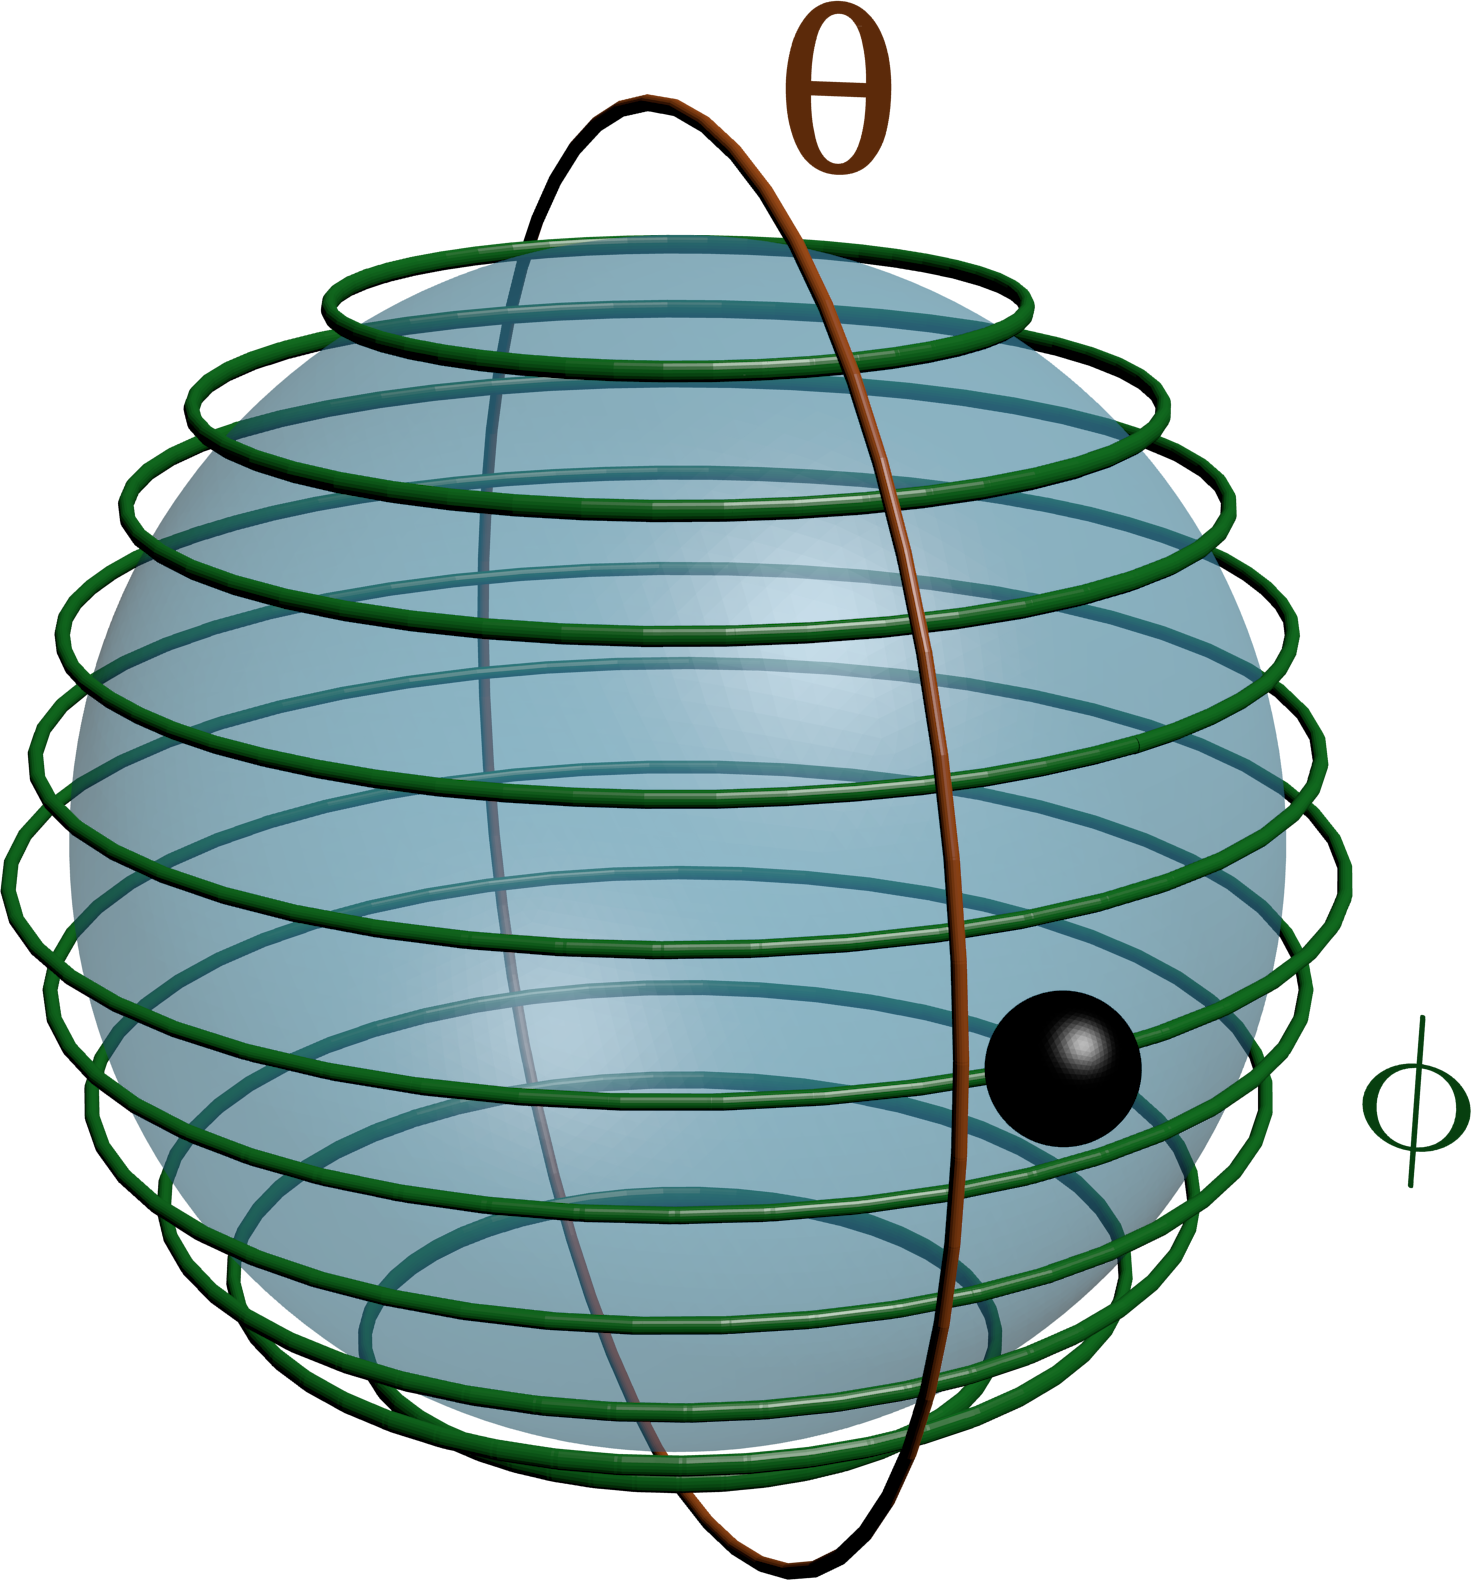
\includegraphics[width=\linewidth]{particle_on_sphere_rings}
\end{wrapfigure}
A very pleasant way to think about why the equation is separable into a part that depends on $\theta$ and a part that depends on $\phi$ is to imagine that the sphere is composed of a series of concentric rings. Our particle can rotate around each ring (giving the $\phi$ term, like a particle on a ring), but can also \emph{hop between} the rings - this gives the $\theta$ term. This is illlustrated in the adjacent figure. That we can separability is quite powerful if we were going to do any more complicated mathematics with them, but we aren't, so no worries.

The second important aspect is to consider \emph{how} the spherical harmonics solve~\autoref{eq:SE_sphere_alt}. The spherical harmonics satisfy the following relationship:
\begin{equation}\label{eq:spherical_harmonics}
	\Lambda^2Y_{l,m_l} = -l(l+1)Y_{l,m_l}
\end{equation}
Where $l = 0,1,2...$ and $m_l = -l, -l+1...l-1,l$. We will discuss the physical interpretations of $l$ and $m_l$ in a second, but first try to compare the above equation to~\autoref{eq:SE_sphere_alt}:
\begin{align*}
	\Lambda^2Y_{l,m_l} &= -l(l+1)Y_{l,m_l} \tag{\ref{eq:spherical_harmonics}}\\
	\Lambda^2\wf_{R} &= -\frac{2IE_R}{\hbar^2}\wf_R \tag{\ref{eq:SE_sphere_alt}}
\end{align*}
Comparing these two equations should lead us to two conclusions. Firstly, the wavefunctions, $\wf_R$, are given by the \emph{spherical harmonics}, that is:
\begin{equation}
	\wf_R(\theta,\phi) = Y_{lm_l}(\theta,\phi)
\end{equation}
Secondly, comparing the terms on the right hand side (knowing that already that $\wf_R = Y_{lm_l}$) leads us to be able to state:
\begin{equation}
	-l(l+1) = -\frac{2IE_R}{\hbar^2}
\end{equation}
Rearranging, we can find an expression for the energy $E_R$:
\begin{equation}
	E_R = l(l+1)\frac{\hbar^2}{2I}
\end{equation}
Which might be starting to look like something a bit familiar from rotational spectroscopy? We are now in a position to discuss what the physical interpretation of $l$ and $m_l$ is, but before we do, lets quickly discuss the \emph{spherical harmonics} and where you have seen them before. 

\subsection{Aside - The Spherical Harmonics and Atomic Orbitals}
Maybe you don't think you've seen the spherical harmonics before, but you have! If I imagined that my particle on a sphere was actually an electron floating around an atom, I could go through all the maths that we just went through and figure out what the \emph{wavefunctions for that system} looked like. We know that the wavefunctions for this system are given by the \textbf{spherical harmonics}, and in the figure below I've plotted the first few spherical harmonics - do they look familiar?

\begin{figure}
	\centering
	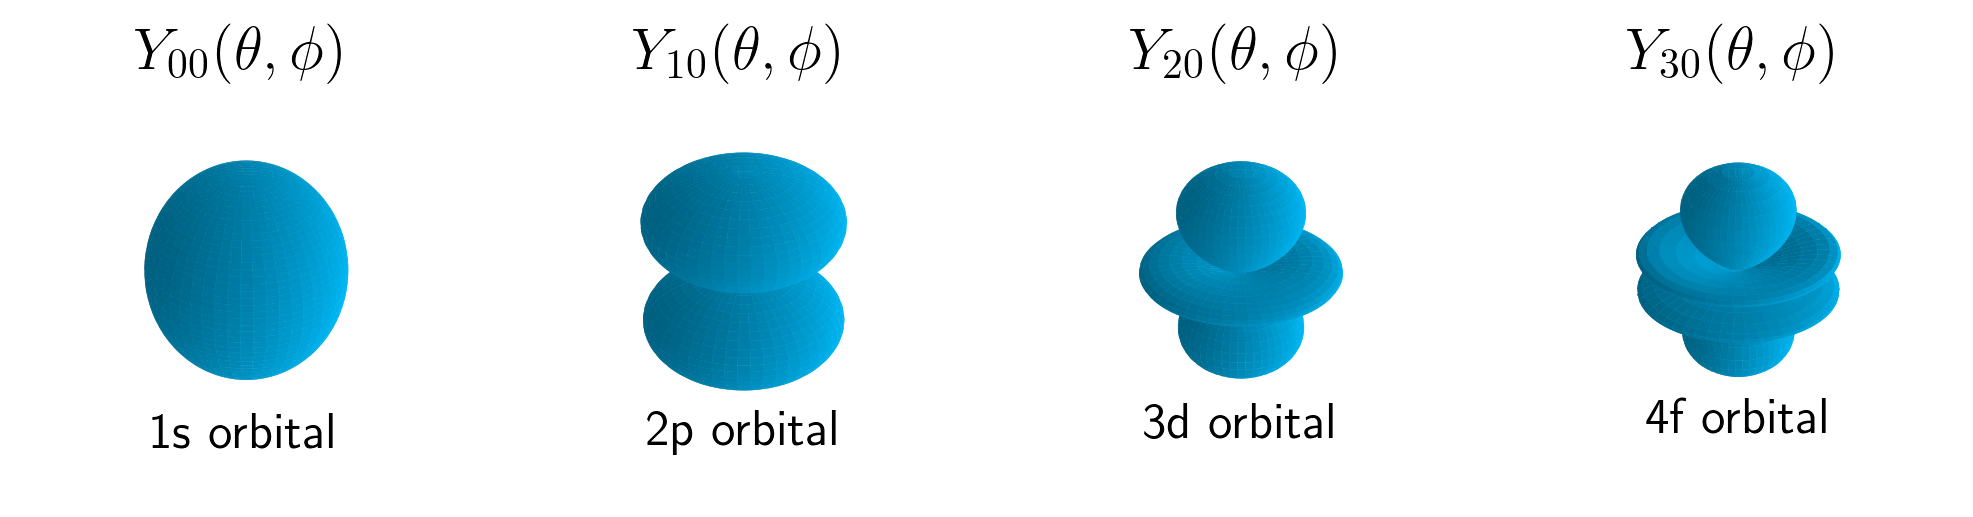
\includegraphics[width=\textwidth]{./spherical_harmonics/spherical_harmonics}
\end{figure}

This looks quite a bit like an s, p, and d orbital, doesn't it? That's because it is (as the labelling shows)! The key point here is that \textbf{the shapes of atomic orbitals are the shapes of the wavefunctions of the electrons that inhabit them.} By treating our electron like a particle on a sphere, we can derive these orbitals just from the quantum mechanics - isn't it remarkable?

This also can shed some new light on the meaning of the angular momentum quantum numbers, $l$ and $m_l$. We will discuss this in a lot more excruciating detail below, but we can see in the figure above that the $s$ orbitals correspond to an angular momentum quantum number $l$ of zero, p orbitals correspond to $l=1$ and d orbitals to $l=2$. How many different degenerate p orbitals are there for each atom? The answer is three - \textbf{one for each of the possible values of $m_l$}. Similarly, there are five degenerate d orbitals for each atom, again one for each possible value of $m_l$. If extended the picture above to f orbitals, how many different degenerate f orbitals would we have?

Anyway, this is all fun, but lets get back to the \textbf{serious quantum mechanics.}

\subsection{The Angular Momentum Quantum Numbers, $l$ and $m_l$}
From our discussion of a particle on a ring, we showed that $m_l$ was a quantum number which told us about the \textbf{magnitude of the angular momentum along the $z$ axis}. In the case of a ring, this was the only angular momentum we had to think about, because we were confined to the ring (only one axis of rotation). Now we can rotate with two angles, $m_l$ alone is \textbf{insufficient} to characterise our entire angular momentum. We saw that we also have another quantum number, $l$. The existence of these two quantum numbers (rather than just one) can be thought of as arising from the fact that we now have to \textbf{satisfy two cyclic boundary conditions, one for $\phi$ and one for $\theta$}.

So what do $l$ and $m_l$ actually mean? Looking at our expression for $E_R$ above, and remembering our definition of rotational kinetic energy from~\autoref{tab:lin_ang}, we can write:
\begin{equation}
	E_R = l(l+1)\frac{\hbar^2}{2I} = \frac{l(l+1)\hbar^2}{2I} = \frac{\text{(angular momentum)}^2}{2I}
\end{equation}
So we can clearly see that our total angular momentum is given by $\hbar\sqrt{l(l+1)}$. We also saw that the definition of the spherical harmonics requires that $l=0,1,2...$. This means that \textbf{angular momentum is quantised}, and therefore $l$ is referred to as the \textbf{angular momentum quantum number.} 

The other quantum number, $m_l$ is called the \textbf{$z$ component of angular momentum} and has values ranging from $-l$ to $+l$ in integer steps. Each specific $l$ level has it's own set of $m_l$ values. For example, the state with $l=1$ can have $m_l = -1,0,1$, and the state with $l=2$ can have $m_l = -2,-1,0,1,2$. Overall, each $l$ state is has $2l+1$ different $m_l$ sub-states. The energy of the different $m_l$ doesn't affect the overall energy (as $m_l$ doesn't appear in our expression for $E_R$), and so the $2l+1$ $m_l$ states are all \textbf{degenerate}. If states are \textbf{degenerate}, it means that they \textbf{have the same energy}. This is all summarised in the table below.
\begin{table}[h]
\begin{tabular}{@{}lll@{}}
\toprule
Quantum Number & $l$ & $m_l$ \\ \midrule
Physical Meaning & Total Angular Momentum & Component of Total Angular Momentum directed along $z$  \\
Allowed Values & $0,1,2,3...$ &  $-l,-l+1,..,0,..l-1,l$ with $2l+1$ states per $l$ level  \\
Affects Overall Energy? & Yes & No (states are $2l+1$-fold degenerate) \\ \bottomrule
\end{tabular}
\end{table}

I promised to explain what these two quantum numbers physically represented, and I have sort of done that, but you're probably still thinking `I don't think you have'. It will become clearer in the following section as we discuss an illustrative model for angular momentum quantisation called \textbf{The Vector Model}.

\subsection{The Vector Model}
Before we embark on this discussion, it's probably useful to revise some mathematics that you may have forgotten. We stated earlier that $m_l$ was the ``$z$ component of the angular momentum'', which can be restated as ``the component of the angular momentum that lies along the $z$ axis'', or as the ``\textbf{projection} of the total angular momentum onto the $z$ axis''. Let us consider what this means.

If you did A level physics (or mechanics in maths), you might recall that we can write a force $F$ acting in the $(x,y)$ plane as the sum of two components, $F_x$ and $F_y$. Here, $F_x$ is the \textbf{component} of the force $F$ that acts along $x$, and $F_y$ is the \textbf{component} of the force $F$ that acts along $y$. This is illustrated in the figure below for three different forces, $F_1$, $F_2$, and $F_3$. $F_1$ is directed mostly along the $y$ axis, so the $y$ component is the largest. Conversely, $F_3$ is directed mostly along the $x$ axis, so the $x$ component is the largest. Finally, $F_2$ is directed at 45 degrees to both axes, so the $x$ and $y$ components are equal. Breaking down the force into it's individual \textbf{components} can be a powerful way to understand what is happening. We could also say that we are \textbf{projecting} the forces onto the $x$ and $y$ axes - which means the same thing as breaking them into components. Imagine that each force vector is casting a shadow on the $x$ or $y$ axis - the longer the shadow, the greater the amount of that force vector that is directed along that axis. This is what \textbf{projection} means.

\begin{figure}[h]
	\centering
	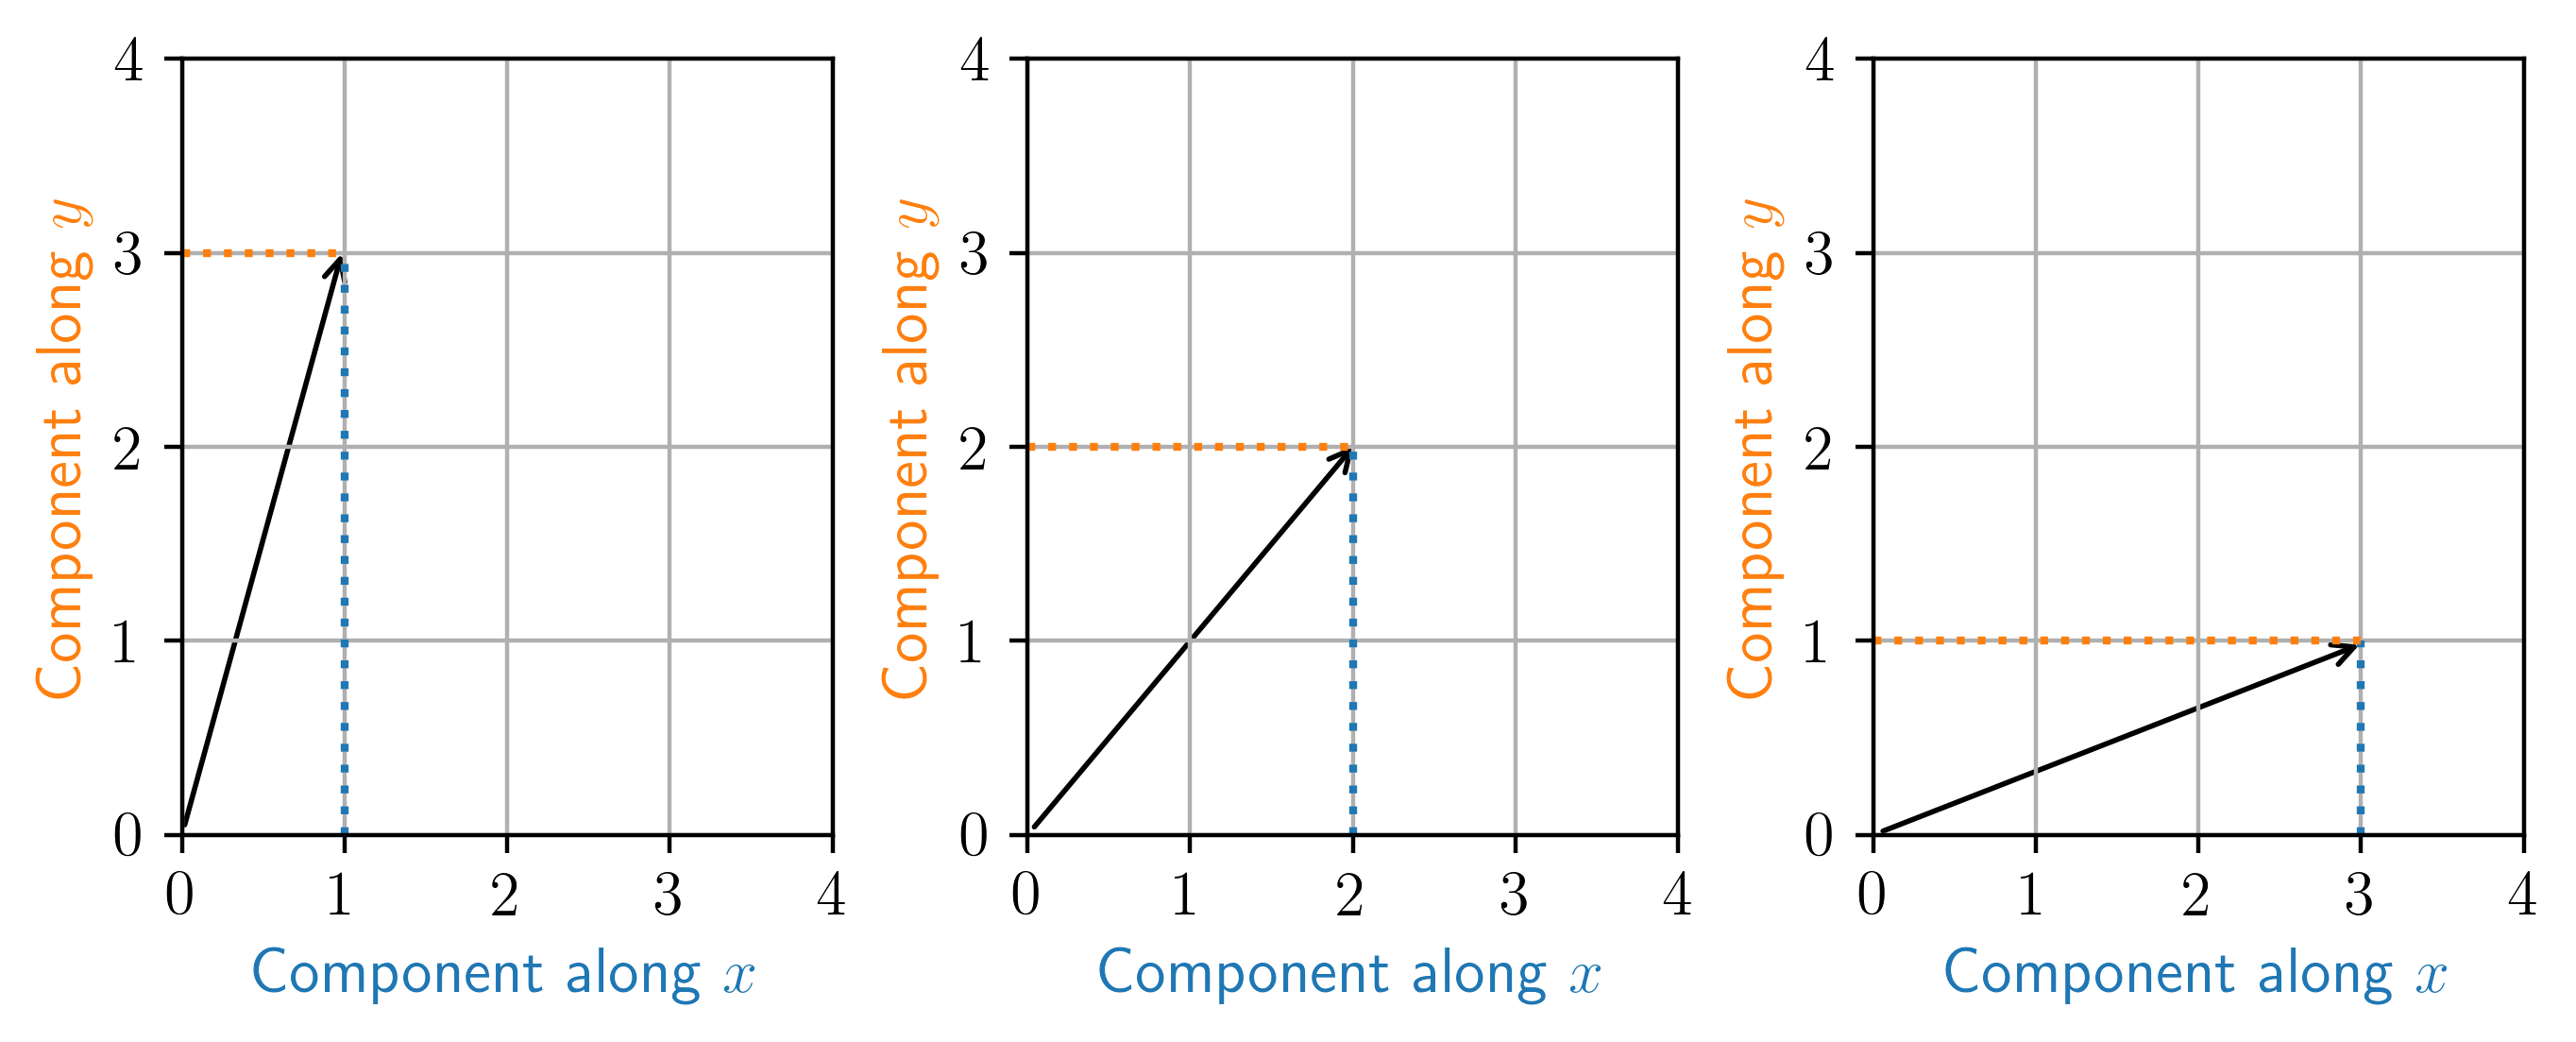
\includegraphics[width=0.9\textwidth]{force_components}
	\caption{A generic vector (shown in black) with it's components along the $x$ (blue) and $y$ (orange) axis labelled.}\label{fig:force_components}
\end{figure}
Why am I telling you this? Well, we can apply this method of \textbf{projection} to \emph{any vector quantity}, not just forces. That means we can apply it to \emph{momentum}, and specifically we can apply it to our \emph{angular momentum}. Is the definition of $m_l$ as the component of $l$ directed along $z$ making more sense? $m_l$ is just the \textbf{projection of $l$ onto $z$}.

Which brings us nicely to something called \textbf{The Vector Model}. To construct this model, we need to remember our expression for the magnitude of the angular momentum that we obtained from our expression for $E_R$:
\begin{equation}
	\text{magnitude of angular momentum} = \lvert l \rvert = \hbar\sqrt{l(l+1)}
\end{equation}
We could imagine the angular momentum, then, as a \textbf{vector} with length $\lvert l \rvert = \hbar\sqrt{l(l+1)}$. We also know that the $z$ component of this vector is given by $m_l$. So, we know how long the vector is, but where does it point?   

We can figure this out if we know the equation which allows us to calculate the $z$ component of an arbitrary vector, $F$. In the co-ordinate system we're using, it's the case that the $z$ component, $F_z$ is given by:
\begin{equation}
	F_z = \lvert F \rvert \cos\theta
\end{equation}
%\begin{wrapfigure}{r}{0.25\textwidth}
%	\centering
%	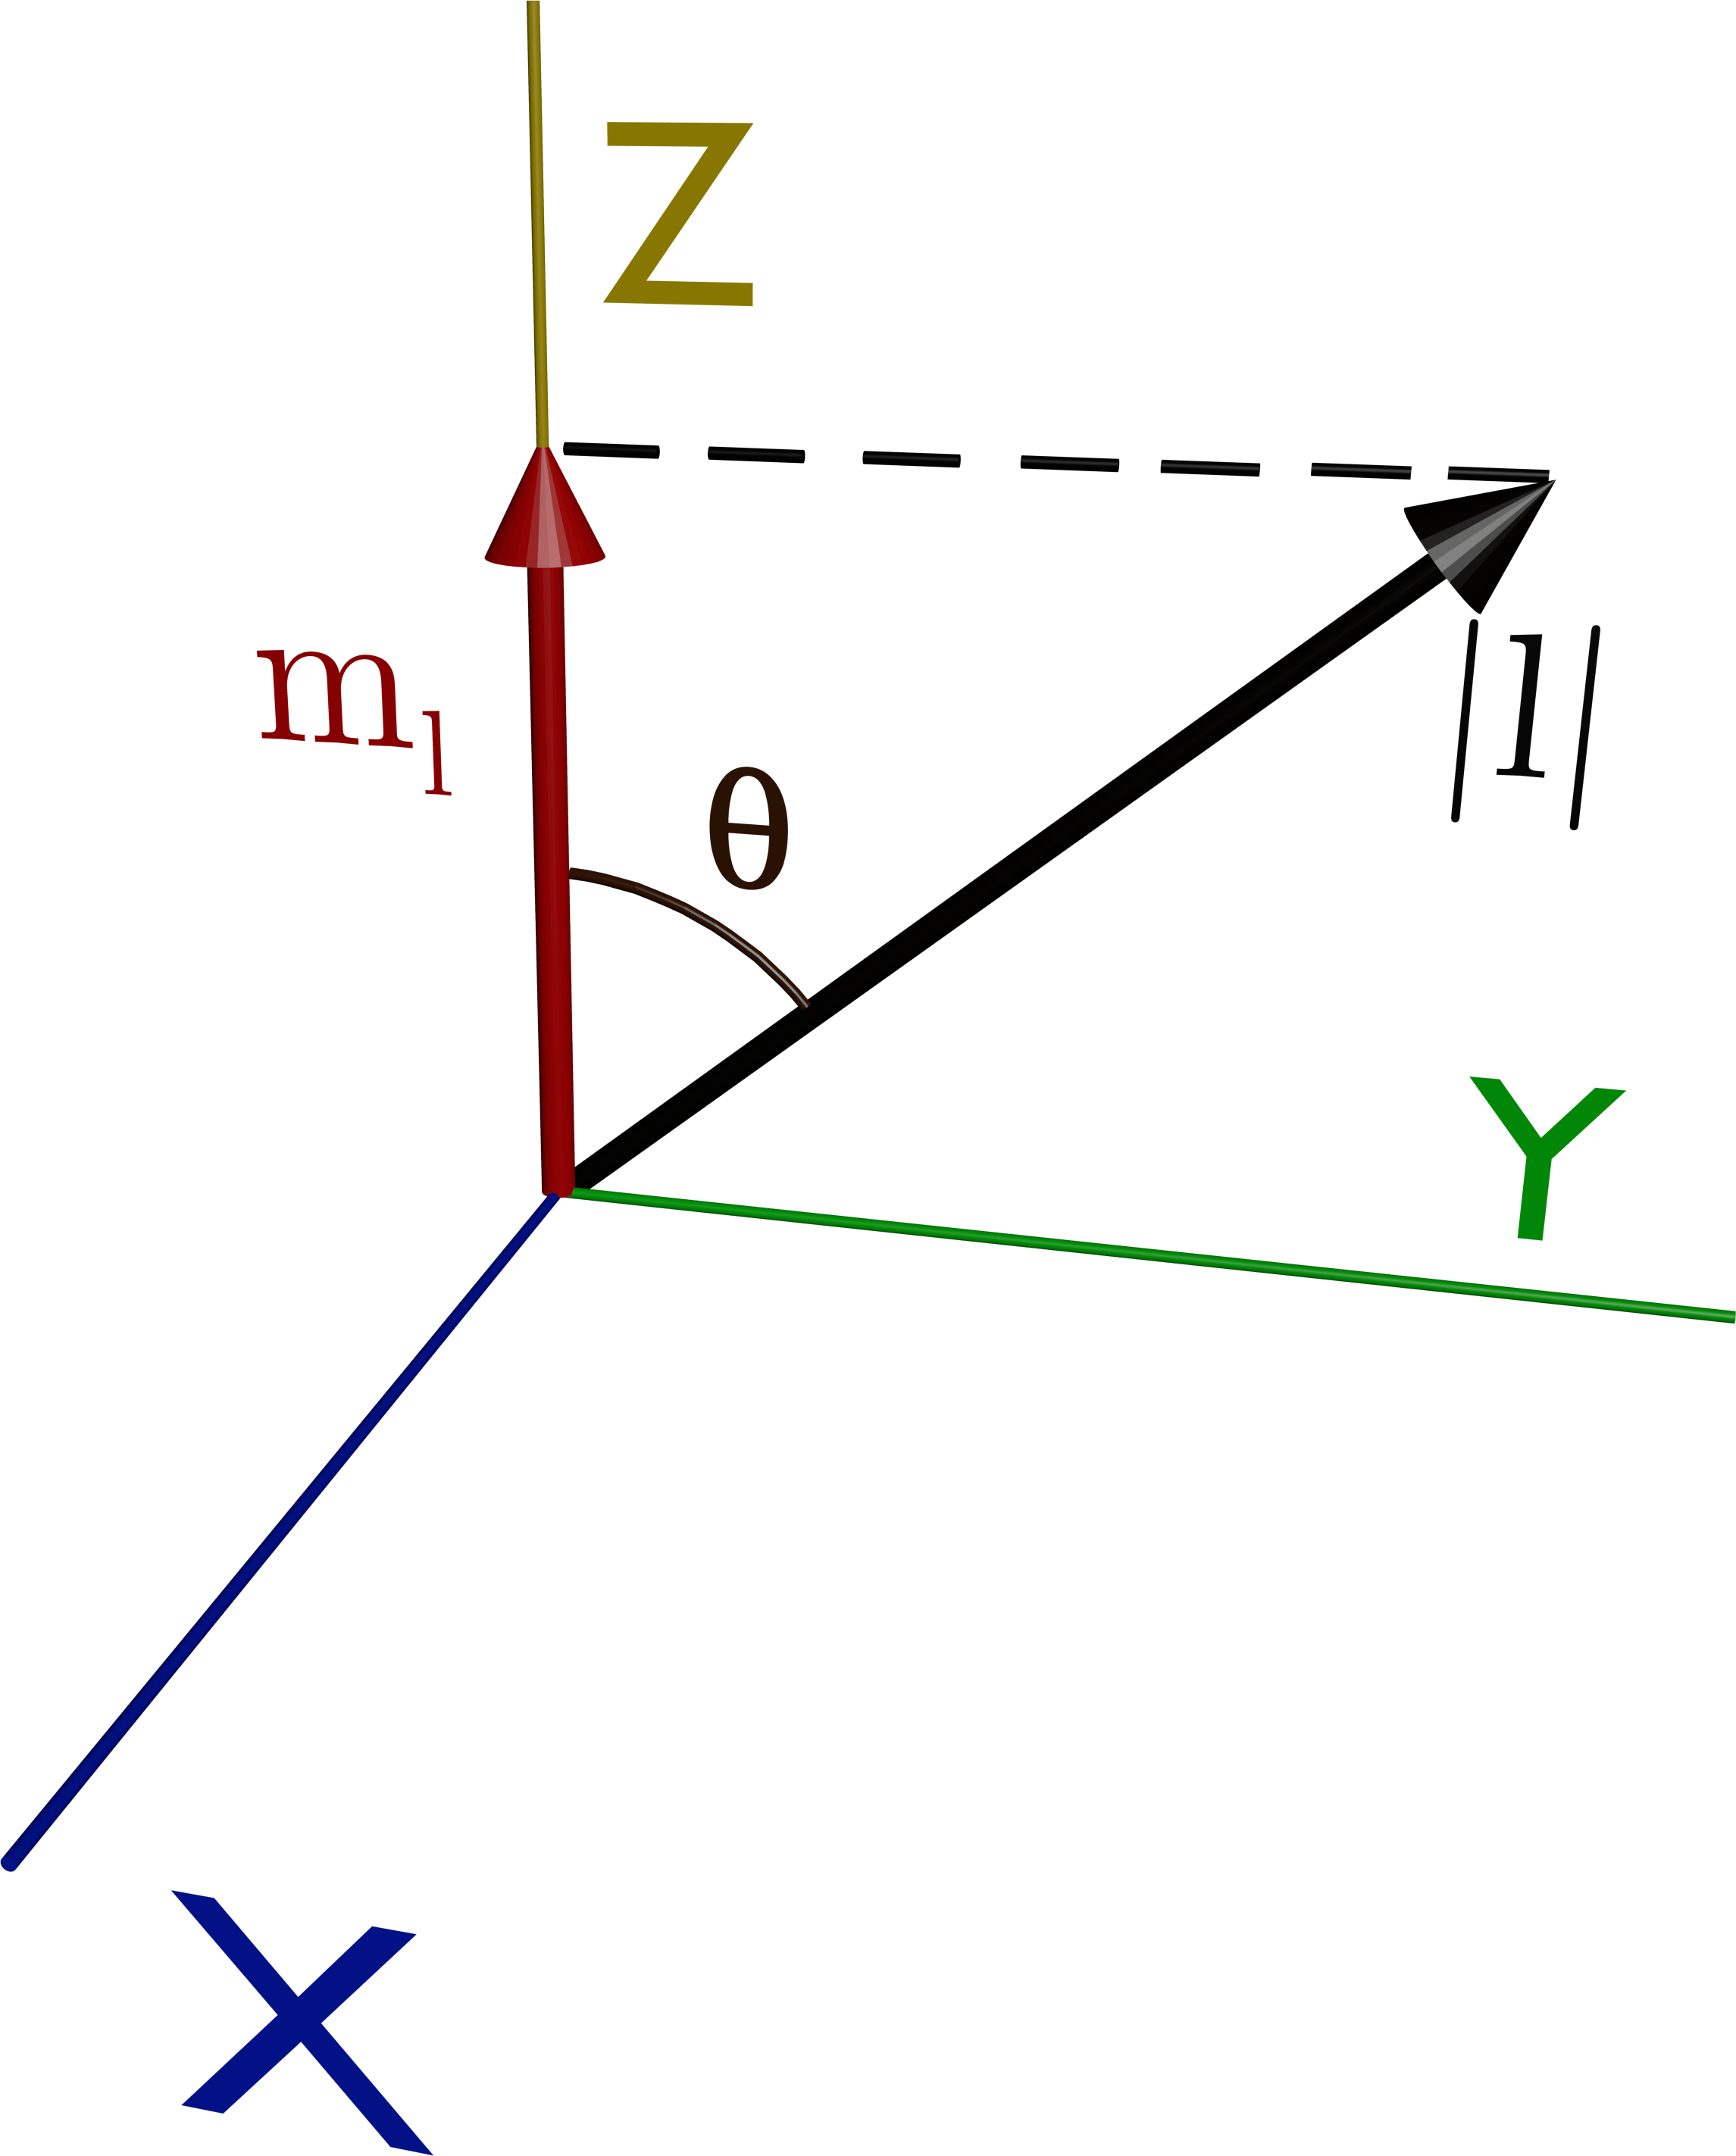
\includegraphics[width=\linewidth]{space_quantisation}
%	\caption{The relationship between an angular momentum vector with length $\lvert l \rvert$ (black) and the projection of that vector onto the $z$ axis $m_l$ (red). $\theta$ is the angle between the vector with length $\lvert l \rvert$ and the $z$ axis.}\label{fig:space_quantisation}
%\end{wrapfigure}
That is, the $z$ component of an arbitrary vector $F$, is given by the product of the \textbf{magnitude} of $F$, $\lvert F \rvert$, and the \textbf{cosine} of the angle $\theta$ between $F$ and the $z$ axis. This is illustrated for our angular momentum vector with length $\lvert l \rvert$ and $z$ component $m_l$ in the adjacent figure.

In our case, we don't know what the angle $\theta$ is (that was what we wanted to work out - where the vector points!), but we do know everything else, so we can say:
\begin{equation}
	m_l = \hbar\sqrt{l(l+1)} \cos\theta
\end{equation}
And we can then rearrange this to give the angle at which our vector points, $\theta$, as:
\begin{equation}
	\theta = \arccos \bigg(\frac{m_l}{\hbar\sqrt{l(l+1)}}\bigg)
\end{equation}

%\begin{wrapfigure}{l}{0.2\textwidth}
%	\centering
%	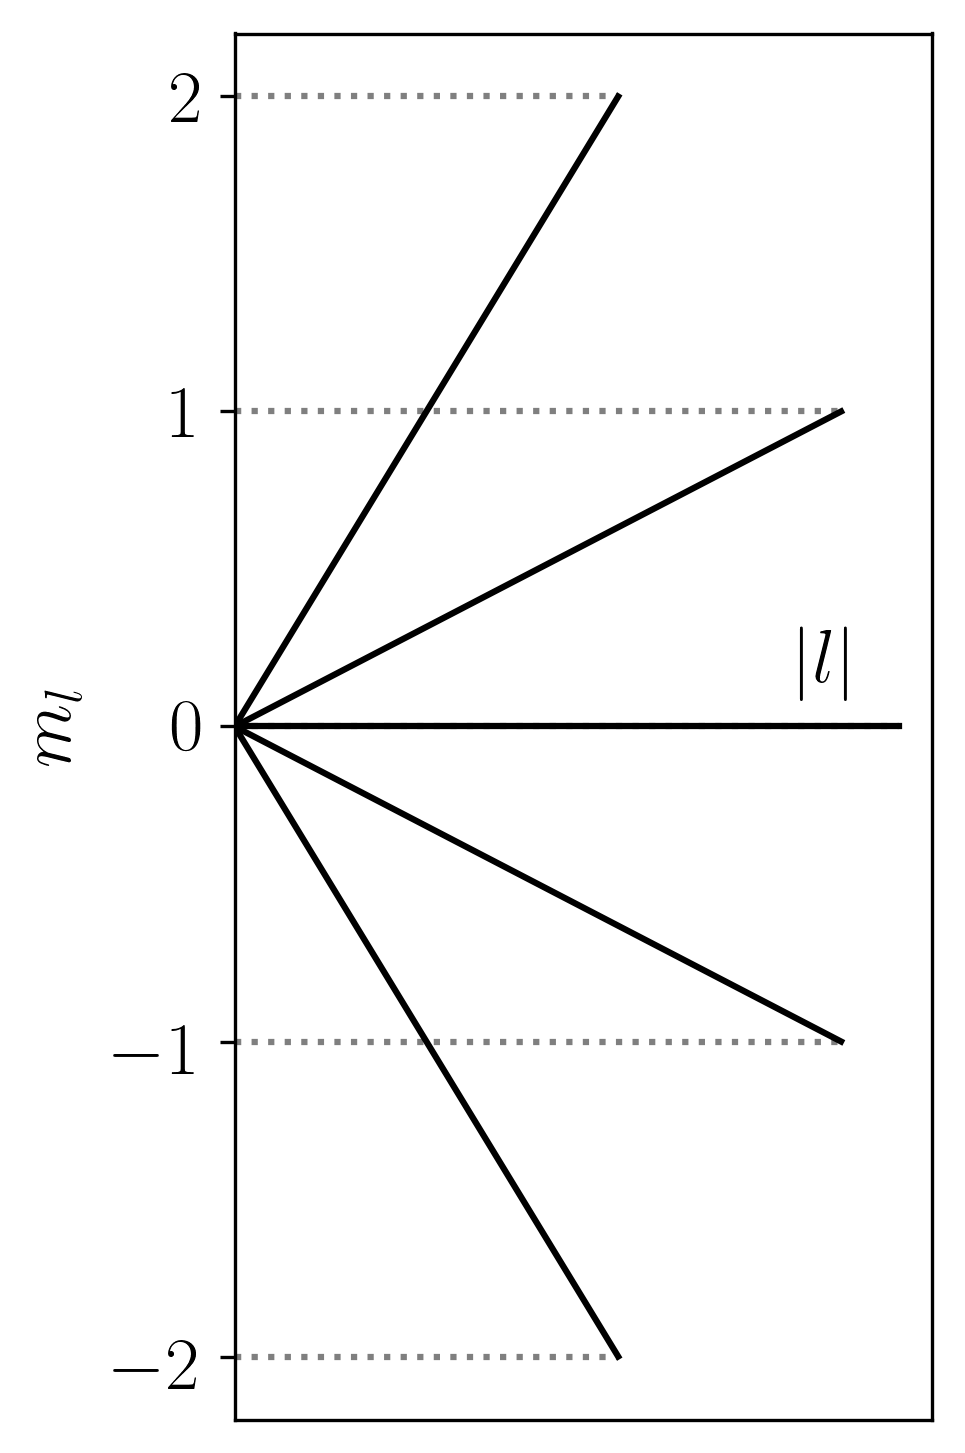
\includegraphics[width=\linewidth]{vector_model}
%	\caption{The Vector Model when $l=2$. Each line represents a possible angular momentum vector with length $\lvert l \rvert$. The vectors can point in $2l+1$ possible orientations, each with a different value of $m_l$.}
%\end{wrapfigure}
The important thing to remember here is that \textbf{$m_l$ is quantised} - we can only have acceptable rotational wavefunctions for specific values of $m_l$. As $m_l$ appears in our equation for $\theta$, it becomes clear our $\theta$ is also quantised - our angular momentum is only allowed to point in specific directions! Classically this doesn't make any sense, as a rotating system can point wherever it wants to. Quantum mechanically, this isn't allowed, and the direction our angular momentum points in is \textbf{quantised}. This is the basis of \textbf{The Vector Model} - illustrated below for when $l=2$.

The physical basis of the vector model was illustrated in~\autoref{fig:space_quantisation}, that we can represent angular momentum as a vector with length $\lvert l \rvert = \hbar\sqrt{l(l+1)}$, with a $z$ component given by $m_l$. As we will have $2l+1$ possible values of $m_l$ for each $l$ state, then each vector will have $2l+1$ different possible $z$ components. This is shown on the adjacent figure for $l=1$ (3 possible $z$ components) and $l=2$ (5 possible $z$ components).  
\begin{figure}[h]
\centering
	\begin{subfigure}[b]{0.35\textwidth}
		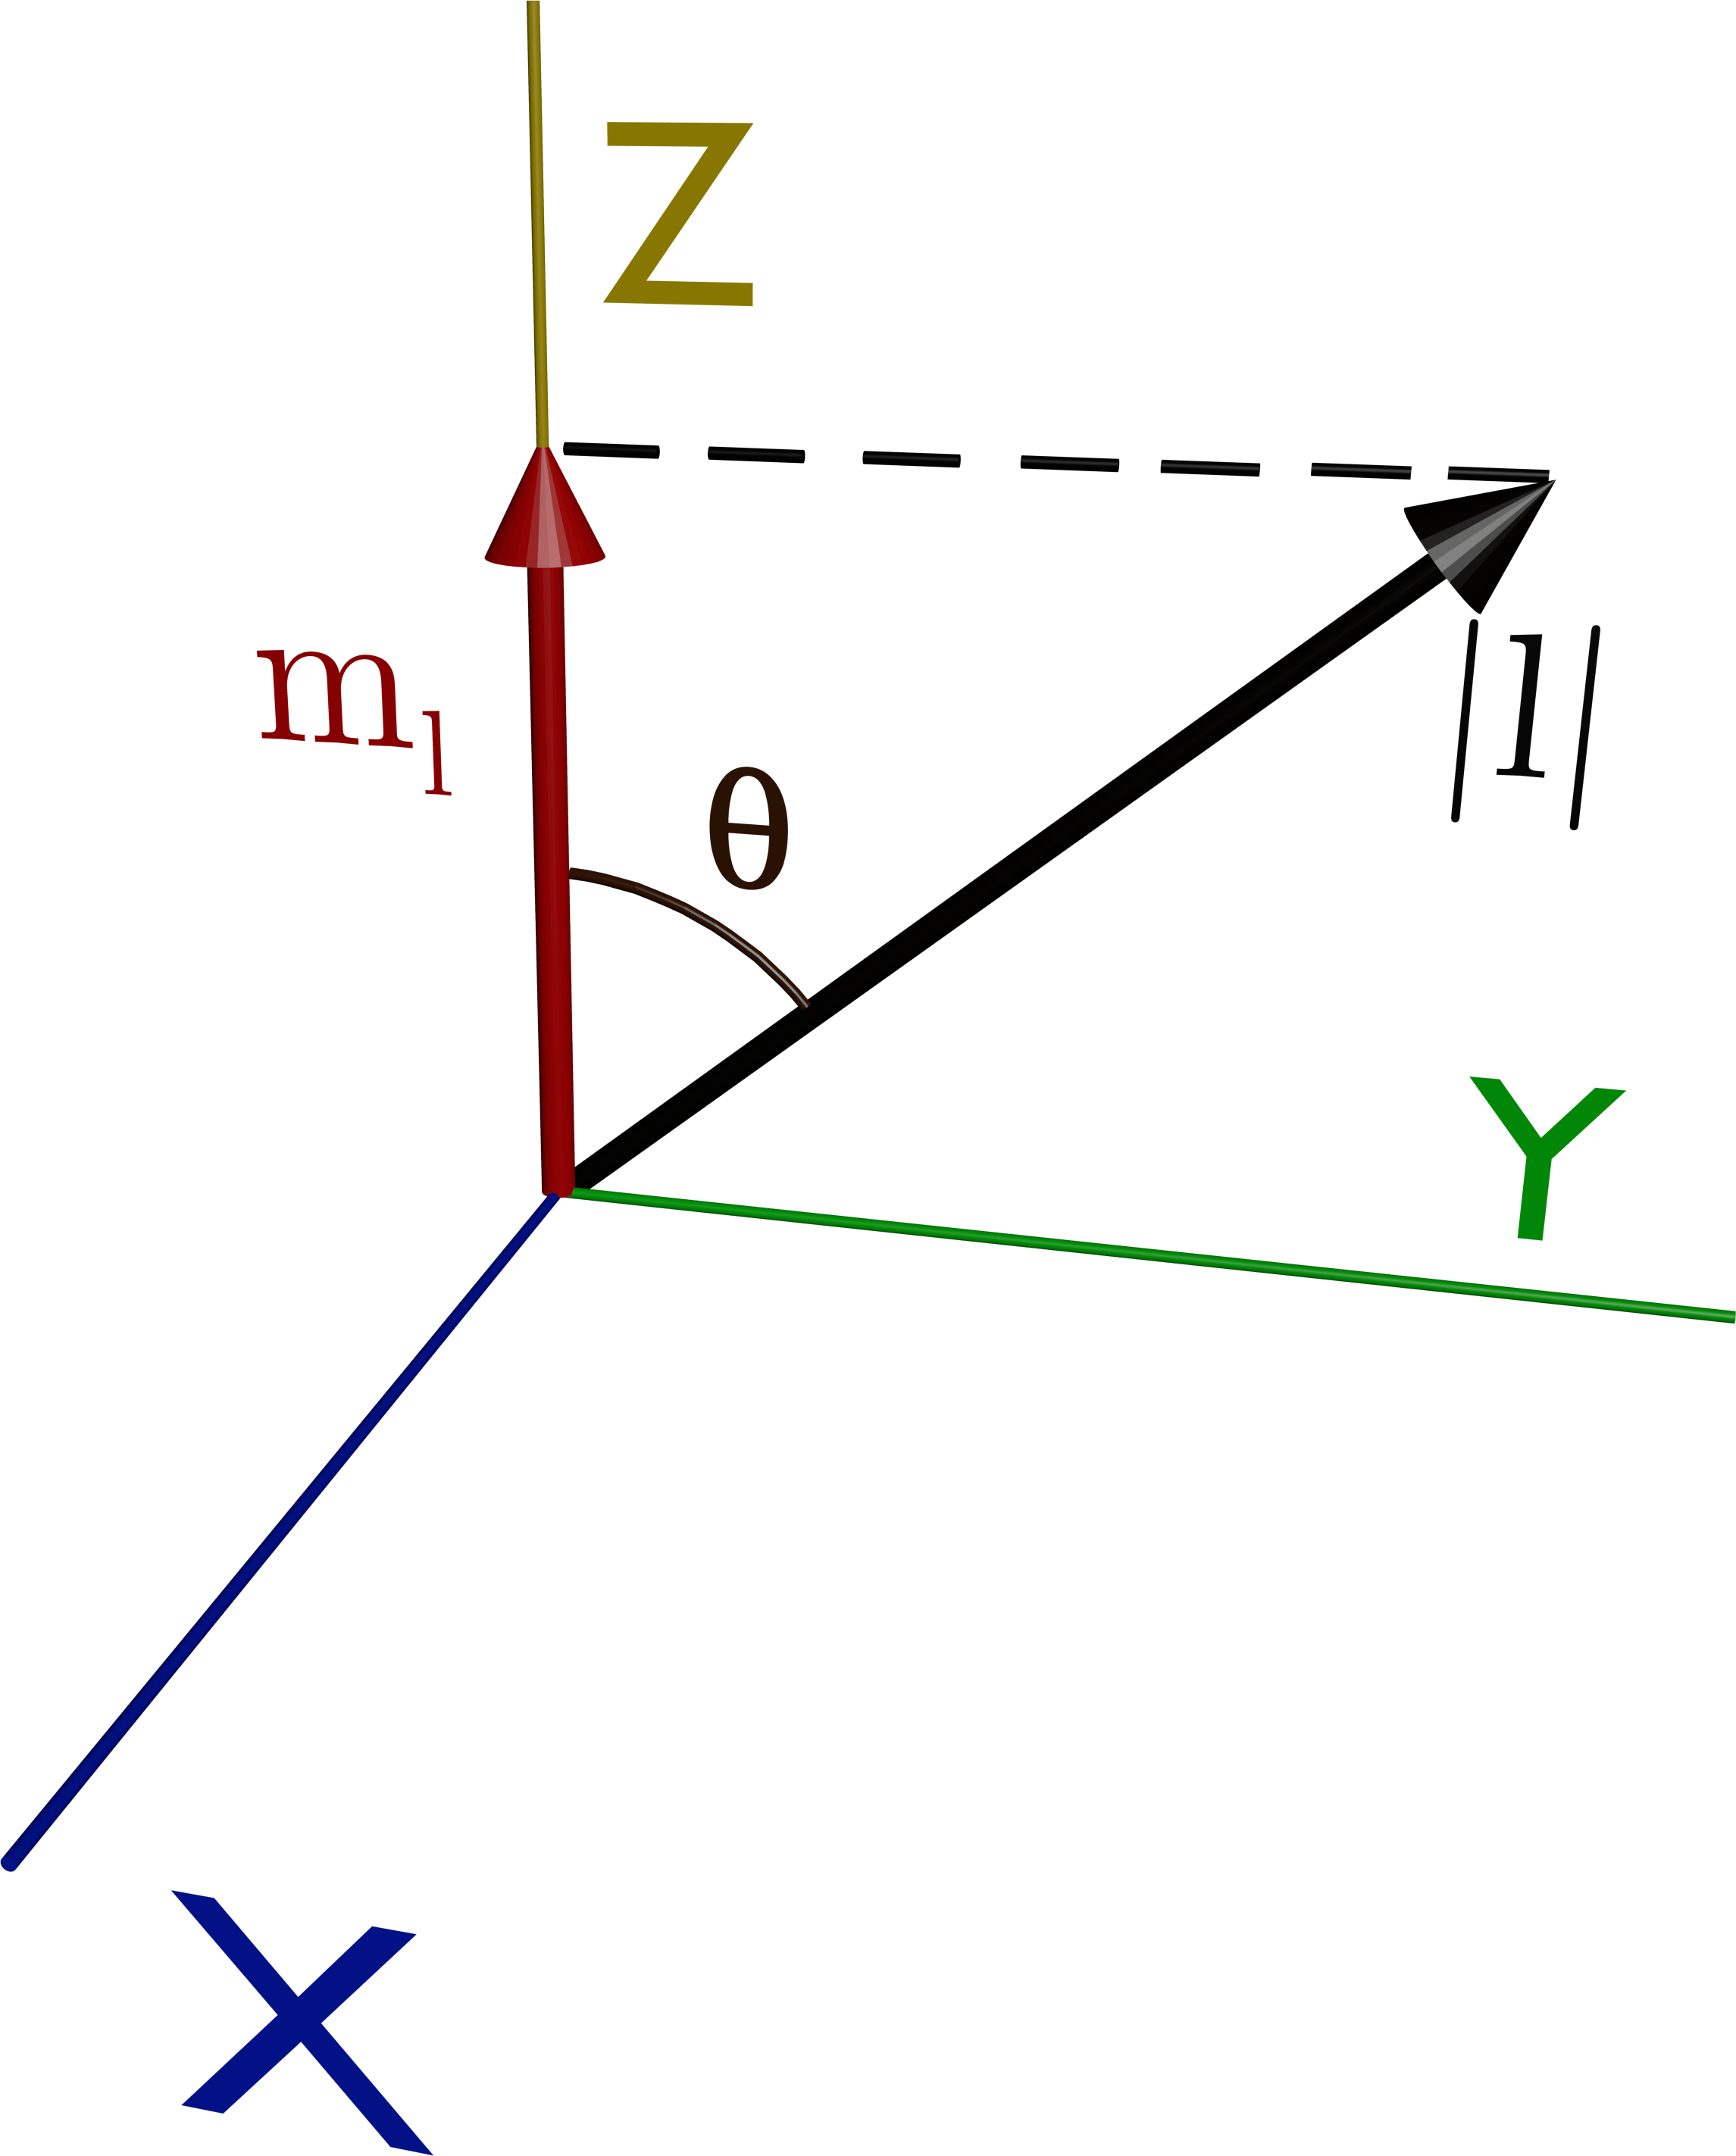
\includegraphics[width=\textwidth]{space_quantisation}
		\caption{The relationship between an angular momentum vector with length $\lvert l \rvert$ (black) and the projection of that vector onto the $z$ axis $m_l$ (red). $\theta$ is the angle between the vector with length $\lvert l \rvert$ and the $z$ axis.}\label{fig:space_quantisation}
	\end{subfigure}
	\qquad
	\begin{subfigure}[b]{0.25\textwidth}
	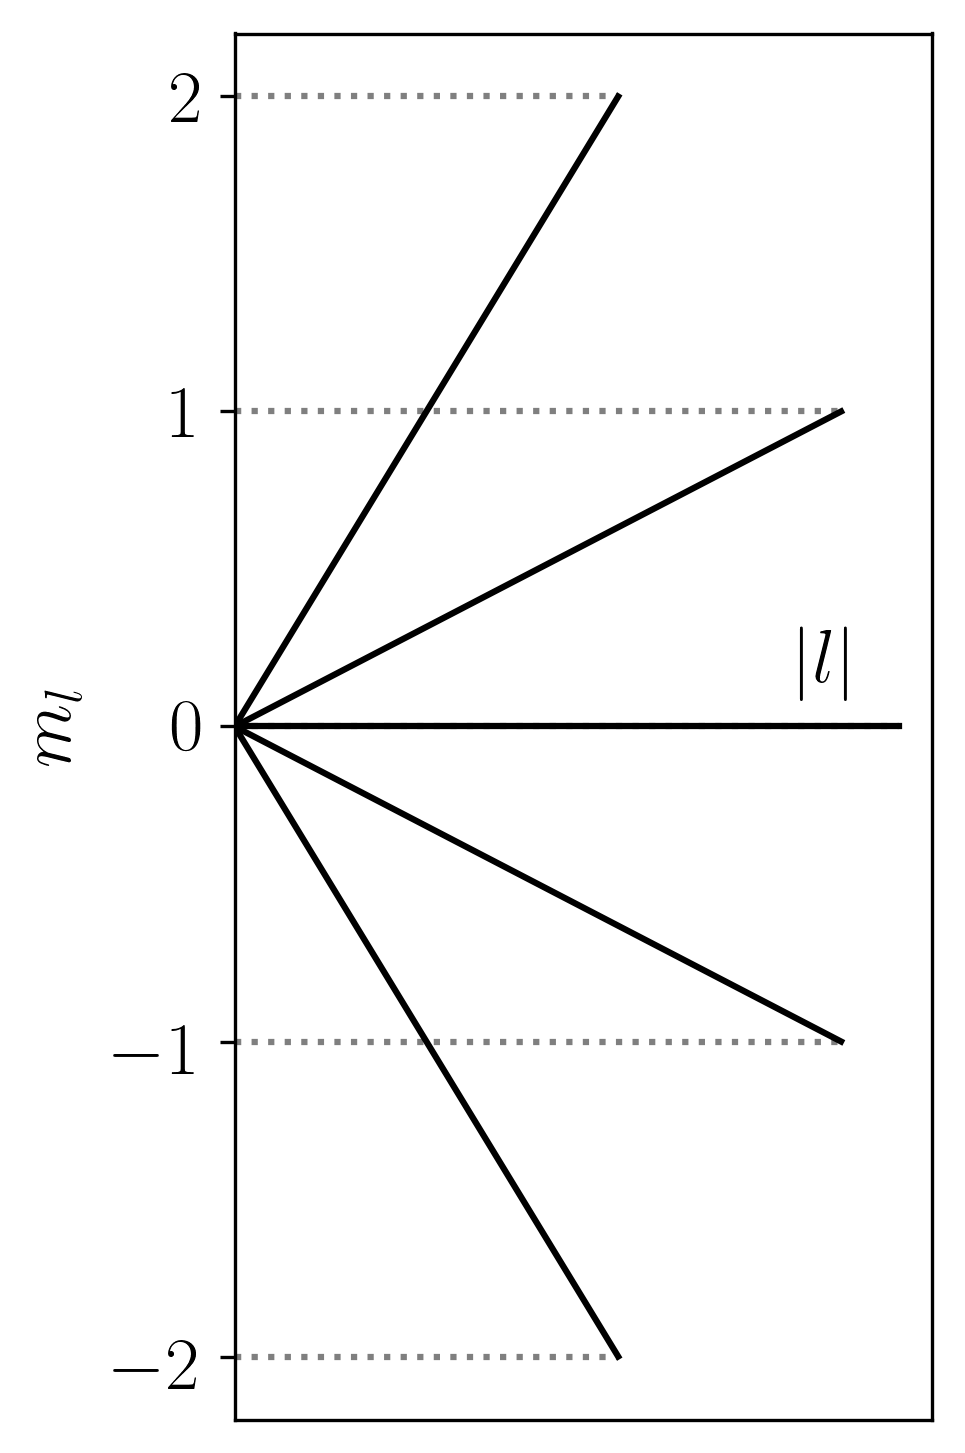
\includegraphics[width=\textwidth]{vector_model}
		\caption{The Vector Model when $l=2$. Each line represents a possible angular momentum vector with length $\lvert l \rvert$. The vectors can point in $2l+1$ possible orientations, each with a different value of $m_l$.}\label{fig:vector_model}
	\end{subfigure}
	\qquad
	\begin{subfigure}[b]{0.25\textwidth}
	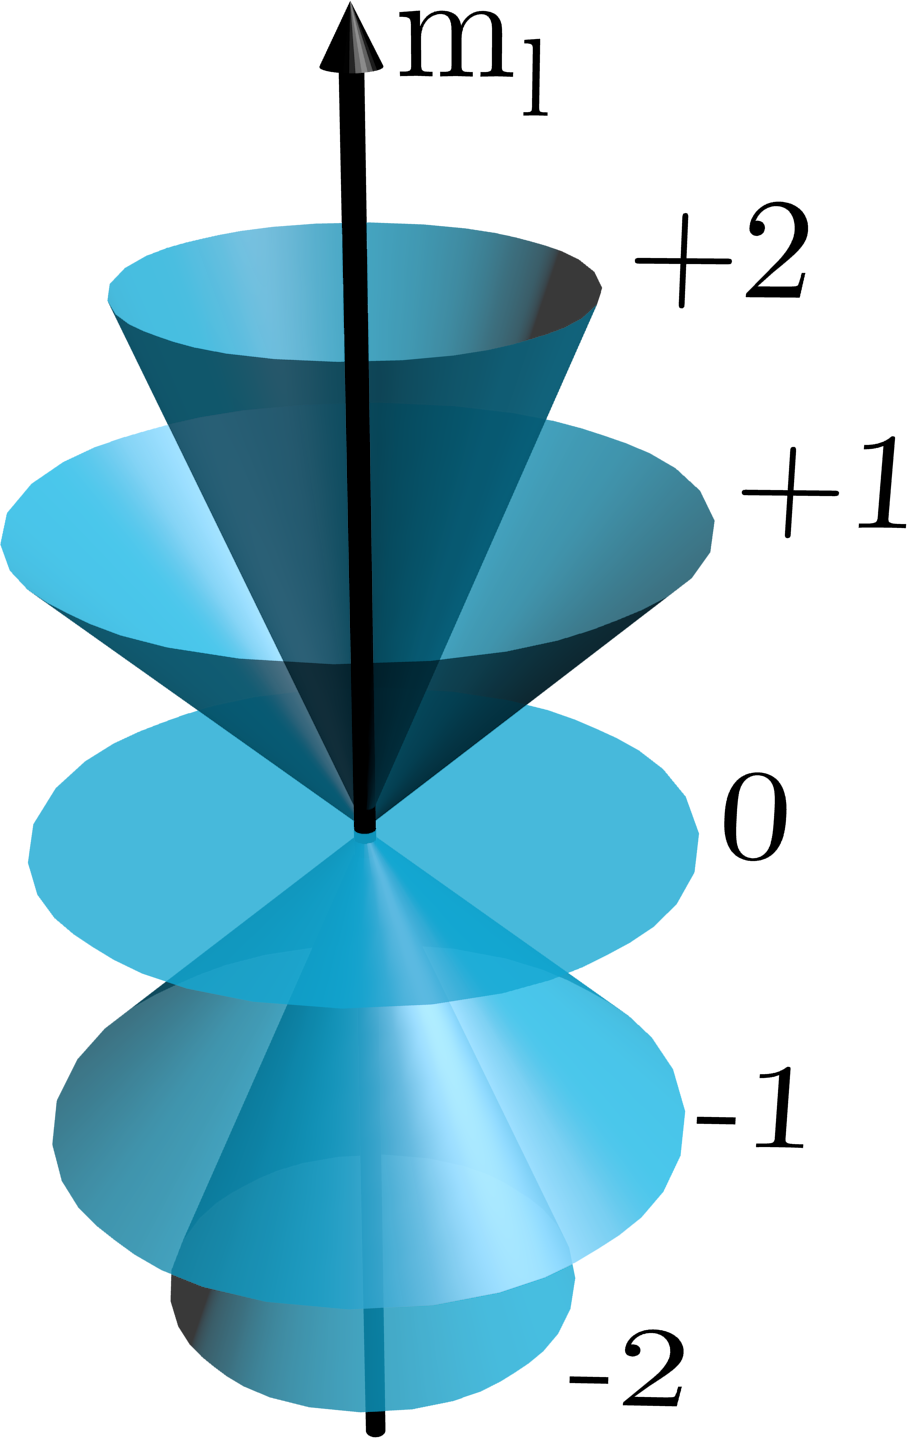
\includegraphics[width=\textwidth]{vector_model_cones}
	\caption{The Vector Model shown as a series of cones. Each cone corresponds to a specific value of $m_l$, and the angular momentum vector can lie in any orientation in the cone.}
	\end{subfigure}
\end{figure}
	
We have spent a lot of this discussion talking about the $z$ component of angular momentum, and it may not immediately be clear as to why we care so much about $z$ and not about the $x$ or $y$ components. The full answer to this question is beyond the scope of this course, but it is to do with the fact that the two quantum numbers $l$ and $m_l$ do not allow us to calculate $x$ and $y$. For this reason, the \textbf{vector model} is often represented as a series of \textbf{cones} corresponding to a specific $m_l$ state. The angular momentum vector $l$ can lie along the surface of any of these cones. 
\vfill
\subsection{Particle on a Sphere Summary}
This was a lot to take in - but we will summarise the most important points below. Angular Momentum is a topic on which huge detailed graduate-level books have been written, so don't feel dismayed if you feel that this is all quite confusing. Angular Momentum is quite confusing - but it \emph{makes the world go around!}


\begin{myblock}{\begin{center}Particle on a Sphere\end{center}}
	\begin{center}
		\begin{align*} & \text{\textbf{Hamiltonian}} \qquad\qquad \hat{H} = -\frac{\hbar^2}{2I}\Lambda^2 \,\quad  \text{where} \quad \Lambda^2 \,\,\text{is the \emph{Legendrian}} \\
			& \text{\textbf{Schr{\"o}dinger Equation}} \qquad\qquad -\frac{\hbar^2}{2I}\Lambda^2 \wf_R(\phi,\theta) = E_R \wf_R(\phi,\theta) \\
			& \text{\textbf{Wavefunctions}} \qquad\qquad \wf_R(\phi,\theta) = \text{The Spherical Harmonics} \\
			& \text{\textbf{Energies}} \qquad\qquad\qquad\qquad\quad E_R = \frac{(\hbar)^2}{2I}l(l+1) \quad \text{where} \quad l=0,1,2,3...
	\end{align*}
	\end{center}
\end{myblock}

If you're very switched on, you may notice that the expression we have here for the energies, $E_R = \frac{\hbar^2}{2I}l(l+1)$, looks a bit like an expression you might be familiar with from rotational spectroscopy:
\begin{equation}
	E = BJ(J+1)
\end{equation}
And there is a good reason for this! We will see why later on, when we apply everything we've learnt to real molecules. It's time to summarise now though.

\section{Chapter 4 Summary}
What I want you to take away from this chapter:
\begin{itemize}
	\item  \textbf{Angular momentum} is the rotational analogue of \textbf{linear momentum}, and can be calculated as the product of the \textbf{moment of inertia} and the \textbf{angular velocity}.
	\item We can make a simple model of rotation in two dimensions with the \textbf{particle on a ring} model. Applying the \textbf{cyclic boundary condition} to this system results in \textbf{quantised angular momentum.}
	\item Extending the rotation into three dimensions with the \textbf{particle on a sphere} system requires application of \textbf{two boundary conditions} and we therefore get \textbf{two quantum numbers}, one for \textbf{total angular momentum} ($l$), and one for \textbf{the z component of angular momentum} ($m_l$). 
	\item The solution to the SE for a particle on a sphere gives the wavefunctions as the \textbf{spherical harmonics.} The familiar shapes of \textbf{atomic orbitals} are the spherical harmonics, where we model the electron in our atom as a particle on a sphere.
	\item \textbf{The Vector Model} is a way in which we can understand and visualise $l$ and $m_l$. 
\end{itemize}

We have now covered all three potential ways in which atoms and molecules can move: \textbf{translation, vibration} and \textbf{rotation}. We've derived expressions for the quantised energies for each type of motion. What remains now is for us to apply what we've shown to actual molecules, and illustrate how these energies can help us understand molecular spectroscopy. To do this, we will start with what my old Professor used to call "The Most Important Approximation in The World" - \textbf{The Born-Oppenheimer Approximation}.

\chapter{The Born-Oppenheimer Approximation}
This will be a fairly short chapter - with a lot less maths than the preceding chapter! The aim here is that you gain an \emph{qualitative understanding} of the Born-Oppenheimer Approximation and why it's useful.

\section{Origins}
The \textbf{Born-Oppenheimer Approximation} (henceforth called `The BOA') is named after Max Born (of `Born Interpretation' fame) and J. Robert Oppenheimer (of `Inventing Nuclear Weapons' fame). Before we discuss what exactly the BOA is, let's discuss why it's necessary.

\textbf{Molecules are complicated.} So complicated, in fact, that even very powerful computers cannot completely analytically and exactly solve the SE for them. The problem is that we have so many different kinds of motion happening inside a molecule, that solving the SE to find the energies of all of them at the same time is completely impossible. Even for something very simple, like a \ce{He} atom (consisting of two protons, two neutrons, and two electrons) is \textbf{far too complex} for us - we couldn't find the energies of everything at once if we tried to. 

The solution, then, is to break the problem down into something more solvable. The thing that really helps us here is to notice that \textbf{different kinds of motion occur on different timescales and with different energies}. An electron is about 2000 times lighter than a proton, so if I gave them each \emph{equal energy}, the proton ends up moving about 200 times slower than the electron (remember that $v \propto \frac{1}{\sqrt{m}}$). This means that, from an electron's point of view, the protons basically \textbf{stay still}. Imagine you are walking forwards whilst a fast jet aircraft flies over you - you look at the jet and it seems to be going \emph{really fast}, but when the jet pilot looks at you, you basically look \emph{stationary} during the time it takes the jet to fly over you. 

This is the fundamental basis of the BOA, which states that:
\begin{quote}
	\textbf{\emph{The nuclear and electronic components of the wavefunction can be separated.}}
\end{quote}

\begin{wrapfigure}{r}{0.25\textwidth}
	\centering
	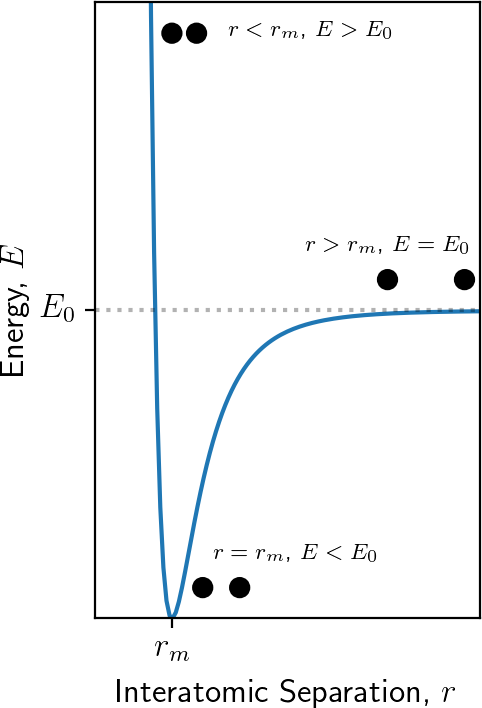
\includegraphics[width=\linewidth]{PES}
\end{wrapfigure}
So what does this mean? It basically means that we can \textbf{treat the nuclei as fixed, and only consider the motion of the electrons}. This makes our job a lot easier, as what we can do is fix our nuclei in space and solve the SE for the electrons, then we can move our nuclei a bit and solve the SE for the electrons with the new nuclear positions. We can then rinse and repeat this process until we have a complete picture of the energies of the molecule!  

In this way, we can produce what is known as a \textbf{molecular potential energy curve}, which is a very important tool for spectroscopists. An example of one is shown in the adjacent figure - it shows us how the energy of a diatomic molecule changes as we change the separation between the two atoms. The lowest energy correspond to the equilibrium bond length, and you can see that as we stretch the bond to large lengths, the energy tends towards zero - \emph{the bond has broken!}

We can combine a series of different \emph{potential energy curves} into a \textbf{potential energy surface}. This is a 3D (or more-D) representation of how the energy of a molecule changes as you change all the bond lengths and angles. Potential energy surfaces can get excruciatingly complex - you might meet them again in the context of kinetics and transition state theory. For now, just be aware that they exist.

Before we proceed, let us just see the mathematical formulation of the BOA. Without the BOA, we would have \textbf{one wavefunction that depends on all nuclear and electronic coordinates}, i.e:
\begin{equation}
	\wf(\text{nuclear},\text{electronic})
\end{equation}
Solving the SE with this wavefunction is impossible - so we invoke the BOA and \textbf{separate the parts}:
\begin{equation}
	\wf(\text{nuclear},\text{electronic}) = \wf(\text{nuclear}) \times \wf(\text{electronic})
\end{equation}
This is now a lot easier to solve, as we can treat both parts separately. The other thing that we tend to do in the BOA is to \textbf{neglect the nuclear kinetic energy} - this makes sense, because we're assuming that the \textbf{nuclei are stationary}. If the nuclei don't move, then they have no velocity or momentum, and therefore no kinetic energy!

\section{Applications to Molecular Spectroscopy}
So, this is all well and good, but we just spent ages talking about translation, vibration, and rotation - so how does this tie into the BOA?

Strictly speaking, if you were a physicist, the BOA only applies to the nuclear and electronic parts of the wavefunction. However, we aren't physicists, so don't need to be shackled into a mundane world where useful approximations aren't allowed because they're `over simplifications'. We said earlier that we can invoke the BOA because nuclei move a lot more slowly than electrons, which means they have very different \textbf{characteristic energies and energy spacings}. In that case, the characteristic energy of electon motion was about 2000 times greater than nuclear motion. The different kinds of motion we've discussed in the previous chapters also \textbf{all have different characteristic energies}. Let us now consider what typical energies each kind of motion may have in a typical molecule. 

Translational energy, which in this case refers to \textbf{moving the whole molecule through space} is quite trivial here. Molecules are generally heavy enough that the energy gap $\Delta E$ between two adjacent translational states is basically zero. We can put the molecule wherever we want in space, and move it around as much as we want! Generally, we can \textbf{neglect the translational contribution to the total energy of the molecule} - as it's pretty much free to move wherever it wants!

Rotational energy is a bit more involved. Generally speaking, the spacing between adjacent rotational level states is not zero. In general, it is somewhere in the region of \SI{1}{\per\centi\metre}. Which is still quite small! You'll see later in the course how to calculate the spacing for typical molecules. 

Vibrational energy has an even greater spacing that rotational energy. Here the spacing between two adjacent levels is somewhere around \SI{1000}{\per\centi\metre}. So we can see that translational, rotational, and vibrational motion all have very different \textbf{characteristic energies}. We could also add in \emph{electronic motion} to this list - which has a greater energy spacing than all the others still (spacing of around \SI{10000}{\per\centi\metre}). This makes our life as spectroscopists quite a lot more straightforward, as we can then say that generally these different kinds of motion don't interact - so we can \textbf{treat them all separately.} This means that we are able to break our typical molecular wavefunction down into constituent parts.
\begin{equation}
	\wf_{\text{Total}} = \wf_{\text{Trans.}} \times \wf_{\text{Rot.}} \times \wf_{\text{Vib.}} \times \wf_{\text{Elec.}}
\end{equation}
Which has the very nice bonus that we are able to write the total energy, $E_\text{Total}$ as:
\begin{equation}
	E_\text{Total} = E_\text{Trans} + E_\text{Rot.} + E_\text{Vib.} + E_\text{Elec.}
\end{equation}
Which is massively important for us as spectroscopists, as it means we are able to treat \textbf{each contribution to the total molecular energy separately}. This means we can think about vibrations without thinking that they might induce rotations, and so on. This is very powerful - as you will understand later.

\section{Chapter 5 Summary}
What I want you to take away from this chapter:
\begin{itemize}
	\item \textbf{The Born-Oppenheimer Approximation} allows us to separate the \textbf{total wavefunction} of a system into \textbf{a nuclear part} and an \textbf{electronic part}.
	\item The approximation relies on the fact that \textbf{nuclear motion happens a lot more slowly than electronic motion}, so we can assume that the \textbf{nuclei are fixed} on the timescale at which the electrons move.
	\item As chemists, we can extend the BOA to say that \textbf{translational, rotational, vibrational, and electronic} motions are all \textbf{separable}. We can do this because each form of motion has a very different \textbf{characteristic energy}.
	\item This allows us to write the \textbf{total wavefunction} as a \textbf{product} of the \textbf{translational, rotational, vibrational and electronic} parts.
	\item Which in turn allows us to write the \textbf{total energy} as a \textbf{sum} of the \textbf{translational, rotational, vibrational, and electronic} parts.
\end{itemize}
Now we move onto the final chapter - which will explain how we can tie all of this together and consider the \textbf{rotational and vibrational quantisation of molecules.} Exciting!

\chapter{Rotational and Vibrational Quantisation of Molecules}
So we are here! In the final chapter of this course. I hope you've enjoyed it so far. What we will do here is apply all the things we've learned to actual molecules and show how we can obtain expressions for the \textbf{energies of spectroscopic transitions} and also derive some of the \textbf{spectroscopic selection rules}.

Before we begin, you'll notice that the title of this chapter doesn't say anything about translations. This is because the translational energy spacings are far too close together to provide us with any spectroscopic insight for any molecule. We spent a lot of time talking about translations purely because it's a nice system to learn the basic quantum mechanics on - it's practical utility is a bit limited in the real world. We can always ignore the translational contribution to the total energy of the molecule.

\section{Spectroscopy}
The overall point of the larger lecture course that this course forms a part of is about learning \textbf{molecular spectroscopy.} At this point, you may have no idea what this actually means (although hopefully you do). \textbf{Molecular spectroscopy} is a thing that we do where we \textbf{shoot radiation at molecules and see what they do}. In this context, \emph{radiation} doesn't mean Chernobyl style nuclear radiation, but rather means things like \emph{microwave, infrared, visible, or ultraviolet} radiation - types of \textbf{electromagnetic (EM) radiation}. Essentially, this is just light of various wavelengths. The \textbf{EM Spectrum} is below, showing different kinds of radiation and what they are useful for. 

\begin{figure}[h]
\centering
	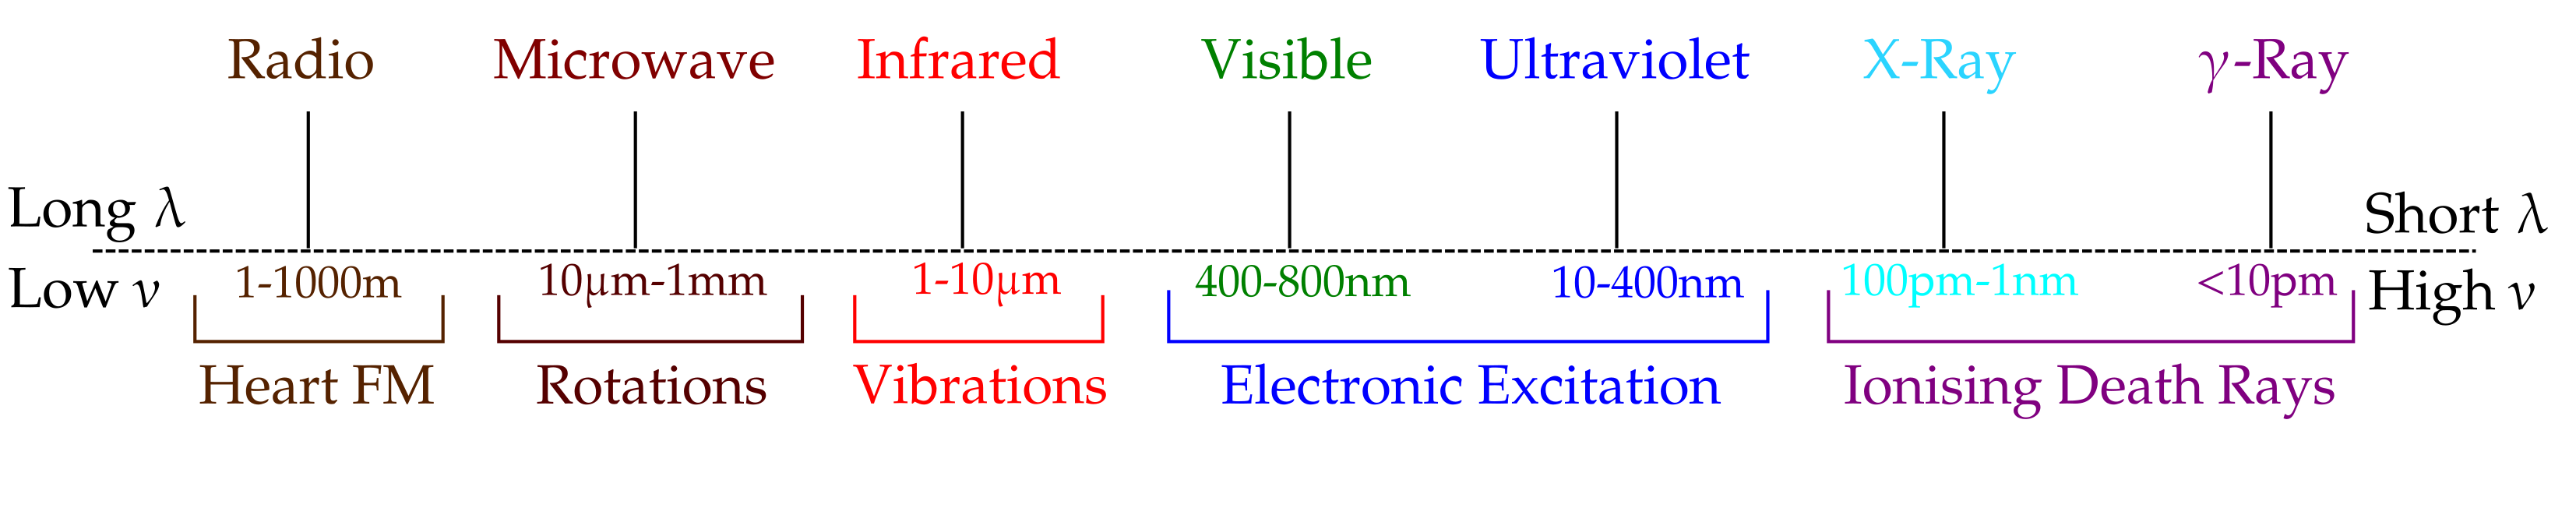
\includegraphics[width=\textwidth]{EM_spectrum}
	\caption{The Electromagnetic (EM) spectrum. Different parts are useful for different things.}
\end{figure}

For example, we might get an infrared laser beam and fire it into a load of molecules and see what they do. If the frequency of the laser beam matches one of the vibrational frequencies of the molecules, the molecule will \textbf{absorb} the infrared radiation and start vibrating. We can then record an \textbf{absorbance spectrum}, which will show us at which frequencies the molecule absorbed the radiation. This spectrum will then tell us about what the \emph{vibrational energy levels} are in the molecules, which in turn can tell us about their structure - as we will see later.

There are a lot of different kinds of spectroscopy, such as infrared, Raman, microwave, UV-VIS, terahertz, VUV, and XUV. However, they all have one big commonality, which is that they involve the \textbf{absorption or emission of photons} (except Raman, which is a story for another time). The energy of the photon that gets absorbed or emitted depends on the \textbf{energy gap} between the states involved in the \textbf{spectroscopic transition}. For example, I could shoot a laser with a photon energy $\hbar\omega$ at a molecule. If that molecule absorbed the radiation, it would undergo a \textbf{transition} from a lower energy state $E_1$ to a higher energy state $E_2$, where:
\begin{equation}
	\hbar\omega = E_2-E_1
\end{equation}
\begin{wrapfigure}{r}{0.3\textwidth}
\centering
	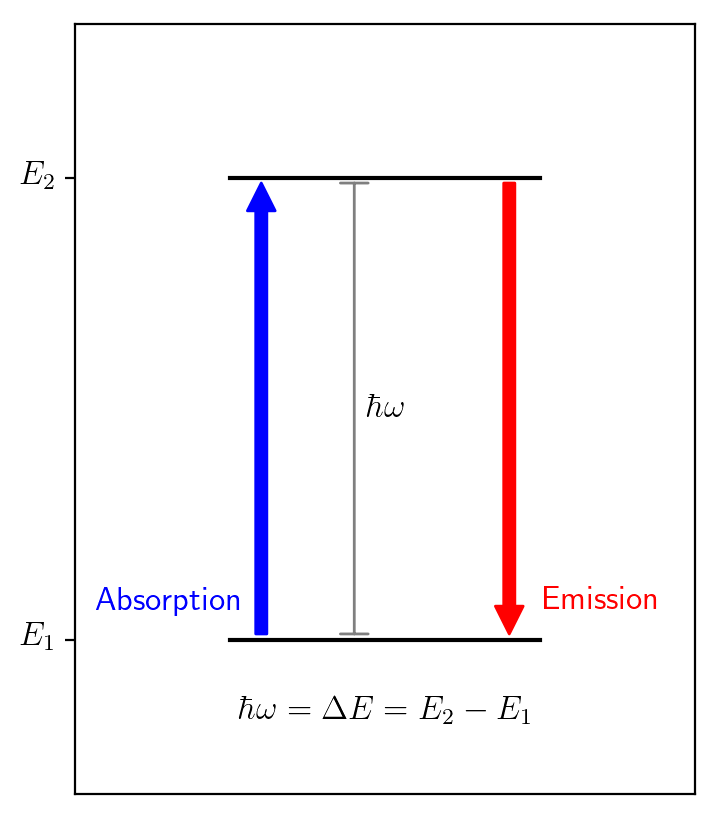
\includegraphics[width=\linewidth]{energy_gap}
\end{wrapfigure}
That is, the \textbf{energy gap} between the states, $\Delta E = E_2 - E_1$, is equal to the \textbf{energy of the incident radiation}, $\hbar\omega$. This relationship is sometimes called the \emph{Bohr Frequency Condition}, after the famous Dane Niels Bohr, and is illustrated in the adjacent figure. This is probably one of the most important equations to know for spectroscopy (although I realise I say that about a lot of equations) - as it provides us with a direct link between the experimental photon energy $\hbar\omega$, and the molecular energy levels $E_1$ and $E_2$. 

So why is this useful? It's all well and good that we can find out molecular energy levels by shooting things with lasers, but why do we want to do that in the first place? The answer is that the \textbf{molecular energy levels depend on molecular properties}. As we will see, we can figure out the energy levels by knowing things like the mass, moment of inertia, bond length, and bond angles in molecules. Conversely, we can then figure out those molecular properties by knowing the energy levels. This is very powerful - and is why spectroscopy is such an important subject! 

\section{Rotational Quantisation}
We're going to start with the hardest case to understand, the \textbf{Rotational Quantisation} of molecules. Once we have this down, it should all be easy! (I hope..)

\subsection{Rotational Energy Levels}
From Chapter 4, we saw that we could find out the \textbf{quantised energy levels} for two systems, the \emph{particle on a ring}, and the \emph{particle on a sphere}. In the former case, we had rotation in 2D (our particle was confined to a ring), and in the latter case, we had rotation in 3D. \textbf{Molecules rotate in 3D}, because they aren't generally glued to the surface of a ring. This means that the \textbf{energies of a rotating molecule are going to be very similar to the energies of a particle on a sphere}, all that changes is the definitions of our moment of inertia, and our angular momentum. 

Taking the moment of inertia first, we saw in Chapter 4 that the main physical property that determined the rotational energy levels was the \textbf{moment of inertia.} Recall that in general the moment of inertia, $I$, for a molecule consisting of $N$ atoms is given by:
\begin{equation}
	I = \sum_{i=1}^N m_ir_i^2
\end{equation}
Where $m_i$ is the mass of atom $i$, and $r_i$ is the distance of atom $i$ from the \textbf{axis of rotation}. We also know from Chapter 4 that the \textbf{rotational kinetic energy} is given by:
\begin{equation}
	E_{\text{Rot.}} = \frac{J^2}{2I}
\end{equation}
Where $J$ is the \textbf{angular momentum} and $I$ is the \textbf{moment of inertia}. If we remember our particle on a sphere, the \textbf{quantised rotational kinetic energy} was given by:
\begin{equation}
	E_{\text{Rot.}} = \frac{l(l+1)\hbar^2}{2I}
\end{equation}
In that case, we used $l$ as our quantum number because we were talking about \emph{orbital angular momentum}. We will now switch to using $J$ as we are talking about \emph{total angular momentum}. I know this can be a bit confusing - just remember that when we talk about rotational energies of molecules \textbf{we use J}. This means we could write our quantised rotational kinetic energy as:
\begin{equation}
	E_{\text{Rot.}} = \frac{J(J+1)\hbar^2}{2I} = \frac{J^2}{2I}
\end{equation}
Which tells us that $J^2 = J(J+1)\hbar^2$. This is an expression for the rotational energy levels of our molecule! However, now we've moved from the abstract world of particles on spheres to the real world of molecules, we need to start thinking carefully about the \textbf{units} of our energies. 

The quantum numbers are all unitless - so that makes life easier. We also know that $\hbar$ has units of \si{\joule\second}. Moment of inertia has units of \si{\kilo\gram\metre\squared}, which would mean that our overall energy has units of \si{\joule\squared\second\squared\per\kilo\gram\per\metre\squared}. If you spent the time, you could see that this simply reduces down to joules, which makes perfect sense! However, it's a lot \emph{more usual} to express our rotational energies in terms of \textbf{wavenumbers}, where a \textbf{wavenumber} is defined as \SI{1}{\per\centi\metre}. We use this slightly odd-looking unit because it gives a nice range of usable numbers when discussing typical spectroscopic transitions. For instance, it's a lot easier to say we have a transition of \SI{10}{\per\centi\metre} (a typical rotational energy spacing), than \SI{0.00124}{\electronvolt} or \SI{1.98E-22}{\joule}. So what we need to do is convert our expression for energy $E_{\text{Rot.}}$ from joules to wavenumbers.

We do this by dividing our expression for energy by $hc$, where $c$ is the speed of light. This gives us the following expression for rotational energy:
\begin{equation}
	E_{\text{Rot.}} = \frac{1}{hc}\frac{\hbar^2J(J+1)}{2I}
\end{equation}
Dividing by $hc$ turns joules into wavenumbers (prove why!). It's now more usual to collect together everything except the quantum numbers and define a new thing called the \textbf{rotational constant}. This is given the symbol $B$ and is defined as:
\begin{equation}
	B = \frac{1}{hc}\frac{\hbar^2}{2I} = \frac{\hbar}{4\pi cI}
\end{equation}
Remebering that $\hbar = \frac{h}{2\pi}$. We can then write our \textbf{rotational energy in wavenumbers} as:
\begin{equation}
	E_{\text{Rot.}}(\text{cm}^{-1}) = BJ(J+1),\quad \text{where:}\, J = 0,1,2...
\end{equation}
Ta da! This is the \textbf{fundamental expression} in rotational spectroscopy. I've deliberately omitted some detail here, but it's in Appendix C if you're interested. You'll meet it later on in the course anyway. Having found this expression, we are in a position to think about what the rotational energies of a typical molecule look like! 

The adjacent figure shows the rotational energy levels of a linear molecule. You can see that the spacing between adjacent levels increases as we increase $J$. This is easily understood if we calculate the spacing between two adjacent levels, $\Delta E_{J,J+1}$
\begin{equation}
	\Delta E_{J,J+1} = E_{J+1}-E_J = B(J+1)(J+2)-BJ(J+1) = 2B(J+1)
\end{equation}
So we can see that the rotational level spacing should increase as $J$ increases. What you may also now ask is, what about the $m_J$ states? We saw for our particle on a sphere that we had another quantum number $m_l$, which could take values of $-l$ to $l$, where there were $2l+1$ possible values for each $l$ state. Why don't we have the same thing here? The answer is that \textbf{we do!} Each $J$ state contains $2J+1$ $m_J$ states - but they are all \textbf{degenerate} (they have the same energy). This degeneracy means that the different $m_J$ states don't really affect what we're doing at the moment, so we will ignore them for now.

\begin{wrapfigure}{l}{0.3\textwidth}
	\centering
	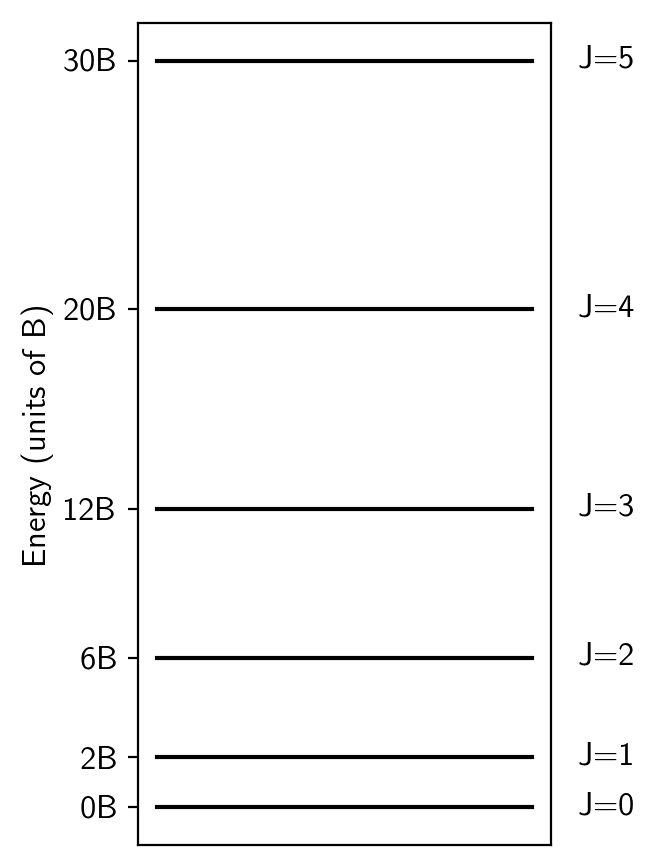
\includegraphics[width=\linewidth]{rotational_energy_levels}
\end{wrapfigure}
Now we know how we can figure out what energies rotational transitions will take - if we know the moment of inertia we can work it out. Conversely, if we measured the transitions, we could figure out a value for the rotational constant, $B$, and therefore the moment of inertia. Can you see how powerful this could be? If we knew, for example, that we had a molecule like \ce{I2}, but wanted to know the exact bond length, we could use $B$ to find the moment of inertia. From the moment of inertia, we can calculate the bond length if we know the masses - which we do, if we know it's iodine! So just from a simple measurement of the energies of the transitions, we can calculate \textbf{useful molecular properties}. However, earlier I alluded to the fact that \emph{not every transition is actually allowed}. This does rather beg the question - \textbf{what transitions are allowed?}

\subsection{Selection Rules and Allowed Transitions}
In a utopian world not governed by the laws of physics, we would be able to shine any light on any molecule and determine any and all of it's properties. However, we don't live in a utopian world and are governed by the laws of physics. Although, if the world was utopian we probably wouldn't need to waste our time doing rotational spectroscopy either. In the real world, not every transition is actually allowed to happen. We can work out which transitions are allowed or not by finding out the \textbf{selection rules}. The selection rules are rules which say things like `only transitions where $J$ increases or decreases by 1 are allowed' and things like that.

You can calculate the selection rules by considering something called the \textbf{transition dipole moment}, or \textbf{TDM}. The TDM is an integral, and a detailed understanding of it is beyond the scope of this course (but some further info can be found in the Appendix). However, as a teaser, this is what the TDM is defined as:
\begin{equation}
	\text{TDM} = \int_{-\infty}^{\infty} \psi_{f}\hat{\mu}\psi_{i} \mathrm{d}\tau
\end{equation}
Where $\psi_i$ and $\psi_f$ are the initial and final states in the transition, and $\hat{\mu}$ is the \textbf{dipole moment operator}. The integral goes over all space, which is what the $\mathrm{d}\tau$ means. Anyway, don't worry about this for now. Just remember what it's called and why it is important.

In general, for a transition to be allowed, the TDM \textbf{has to be non-zero}. When we find the selection rules, we will find that there are two kinds: \textbf{gross selection rules} and \textbf{specific selection rules}. Gross selection rules are selection rules that tell you about the \textbf{general properties a molecule must have to produce a spectrum}. Specific selection rules, in contrast, tell you about \textbf{which specific transitions are allowed in the spectrum}. 

A detailed derivation of the rotational selection rules is unfortunately a bit too complex to set out in detail here. However, I will quote them and we will then see how we can try to understand them physically without going into all the mathematics. The selection rules for rotational transitions (via absorbing or emitting photons\footnote{i.e. not via scattering of photons.}) are: 
\begin{itemize}
	\item Gross Selection Rule: Molecule must possess a \textbf{permanent dipole moment}.
	\item Specific Selection Rule: $\Delta J = \pm 1$.
\end{itemize}
Let's take these in turn and try to understand the underlying physics. 

The \textbf{gross selection rule} can be understood by thinking about how light (EM radiation) interacts with a molecule. Light is just an \emph{oscillating electric field} - imagine a laser beam as being just an area in space where there's a really strong \emph{electric field} oscillating up and down\footnote{It oscillates with the frequency of the radiation, so red light oscillates more slowly than blue light.}. If you put something charged in an electric field, it will move - just like if you put something magnetic in a magnetic field. So, if we put an electron in our laser beam, it would get accelerated up and down as the electric field oscillates, because the charge on the electron gets dragged around as the field moves. Conversely, if we put a neutron in our laser beam, it would just sit there - the electric field has \emph{no effect} on it. So, the EM radiation (the light, or laser beam here) \textbf{interacts with the electrons} on a molecule. 

This explains our gross selection rule. If the molecule in our electric field is polar, there are more electrons on one side of the molecule than the other. This means that one end of the molecule \textbf{feels a greater force from the electric field} than the other end. When this happens, the molecule starts to rotate! Imagine you're holding a car steering wheel - if you have both hands on it and pull down harder on one side than the other, the wheel rotates. Conversely, if you pull \textbf{equally hard} on both sides, then the wheel doesn't rotate. This is what happens to a \textbf{non-polar molecule}. In a non-polar molecule, there's equally many electrons on both sides, so each side \textbf{feels the same force} from the electric field - so \textbf{nothing happens overall!} Therefore, if we want to \textbf{make a molecule rotate} by absorption of photons from EM radiation, it \textbf{needs to have a permanent dipole moment - it needs to be polar}. This is the gross selection rule.

The specific selection rule is a bit harder to conceptualise physically. It's to do with the \emph{conservation of angular momentum} when our molecule absorbs a photon. The simplest way to think about it is to consider a photon of having a single unit of angular momentum. When the molecule absorbs the photon, it absorbs this angular momentum too - so the angular momentum of the molecule has to \textbf{increase by 1}, which means that $\Delta J = +1$ for absorption. By the same argument, if a photon is \textbf{emitted}, the angular momentum of the molecule has to \textbf{decrease by 1}, so $\Delta J = -1$. 

It was briefly mentioned earlier that we're working under the \textbf{`rigid rotor'} approximation - this means that our bond length isn't allowed to change during the rotation (and we therefore can't spin something so fast it starts vibrating). Like most approximations, this is an \emph{approximation}. Later on you will meet things like \emph{centrifugal distortion}, where you account for the bond length changing during a rotation. For now, don't worry about it - but be aware it's a thing.

Let's now summarise the energies and selection rules for rotational spectroscopy, and move onto \textbf{vibrations}.
\begin{myexampleblock}{\begin{center}Rotational Spectroscopy\end{center}}
	\begin{center}
		\begin{itemize}
			\item Energy levels (in \si{\per\centi\metre}): $E = BJ(J+1)$, where: $B = \frac{\hbar}{4\pi cI}$
			\item Gross selection rule: molecule must possess a \textbf{permanent dipole moment}.
			\item Specific selection rule: $\Delta J = \pm 1$.
		\end{itemize}
		\end{center}
\end{myexampleblock}

\section{Vibrational Quantisation}
Now we will consider the case of \textbf{vibrational quantisation}, where we will consider how we can derive energy levels and selection rules for vibrating molecules.

\subsection{Vibrational Energy Levels}
In Chapter 3 we showed that we could derive the energies of a \textbf{quantised harmonic oscillator}. The model we used to explain that was a \emph{mass on a spring}. In that case I hinted that we could consider the spring to be like a chemical bond, so could describe the \emph{vibrations of a bond} in the same way that we described the \emph{vibrations of a mass on a spring}. We will now develop this idea a bit a further. To do this, we will use the concept of the \textbf{reduced mass}. 
\begin{figure}[h]
	\centering
	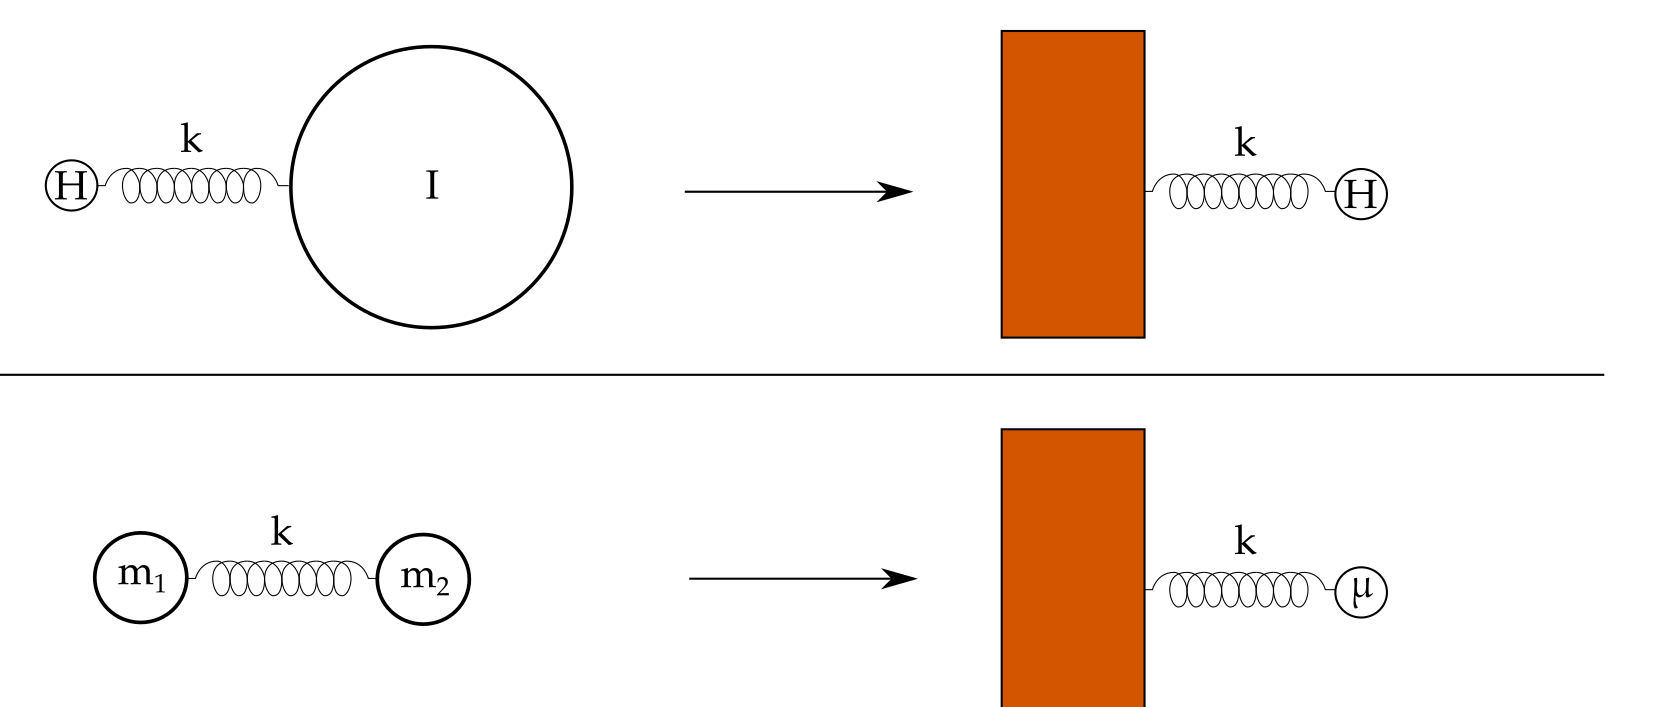
\includegraphics[width=\textwidth]{reduced_masses}
\end{figure}
If we imagine a diatomic molecule, we could consider it to be just \textbf{two masses joined together by a spring}, where the spring is the bond and the two atoms are each mass. So how do we relate this picture to our picture of a single mass on a spring attached to a wall? The answer is that we use the \emph{reduced mass}, which is illustrated above. To understand this, it's useful to consider a diatomic molecule where the two atoms have wildly different masses, such as \ce{HI} - illustrated above. In this instance, the iodine is so enormous and heavy that it's \emph{effectively stationary}, and you can think of the system as just being a hydrogen atom attached to a wall by a spring. 

This is all great, but what happens if the molecule is something like \ce{HF}, or \ce{O2}, where the two atoms have similar (or the same) mass? In that case, we can still consider the system as being a particle attached to a wall, but now the particle attached to the wall has a weight $\mu$, where $\mu$ is the \textbf{reduced mass}, defined as follows (and illustrated in the figure above):
\begin{equation}
	\mu = \frac{m_1m_2}{m_1+m_2}
\end{equation}
So, we can reduce the vibration of any diatomic molecule to just being a mass on the end of a spring, which means we can use all the expressions for the vibrational energy that we derived in Chapter 3! All we have to do is swap out $m$ for $\mu$, as now we're talking about the \textbf{reduced mass of a diatomic} not the \textbf{actual mass of a single particle}. So, our \textbf{quantised vibrational energies} are:
\begin{equation}
	E_v = (v+\frac{1}{2})\hbar\omega,\quad \text{where:}\quad \omega = \sqrt{\frac{k_f}{\mu}},\quad\text{for}\,v=0,1,2...
\end{equation}
This is exactly the same as the equation we derived in Chapter 3, we've just switched out $\mu$ for $m$. $k_f$ is still the \emph{force constant}, and $\omega$ still gives us the \emph{characteristic frequency}. It's interesting to think about what happens to $\mu$ if one of our particles has infinite mass (i.e. it's a wall), and the other particle has mass $m$, then $\mu=m$ - prove that this is true!

Before we proceed - we have to talk about units again! Like before, the expression above will spit out the energy of our vibrational levels in \textbf{joules} (check it and see!). We want the energy in \textbf{wavenumbers} again - so we need to \emph{divide by $hc$ again}. What we normally do is divide it all by $hc$ and then define a new constant called $\tilde{v}$, as follows:
\begin{equation}
	E_v (\text{cm}^{-1}) = (v+\frac{1}{2})\tilde{v},\quad \text{where:}\quad \tilde{v} = \frac{1}{2\pi c}\sqrt{\frac{k_f}{\mu}}
\end{equation}
I think we're now far enough through this course that you can confirm the above is correct yourself! Like the rotational energies in wavenumbers were called \textbf{rotational terms}, these are sometimes called \textbf{vibrational terms} - it's all just analogous. Anyway, having made this small alteration, let's return to the topic at hand.

\begin{wrapfigure}{l}{0.4\textwidth}
	\centering
	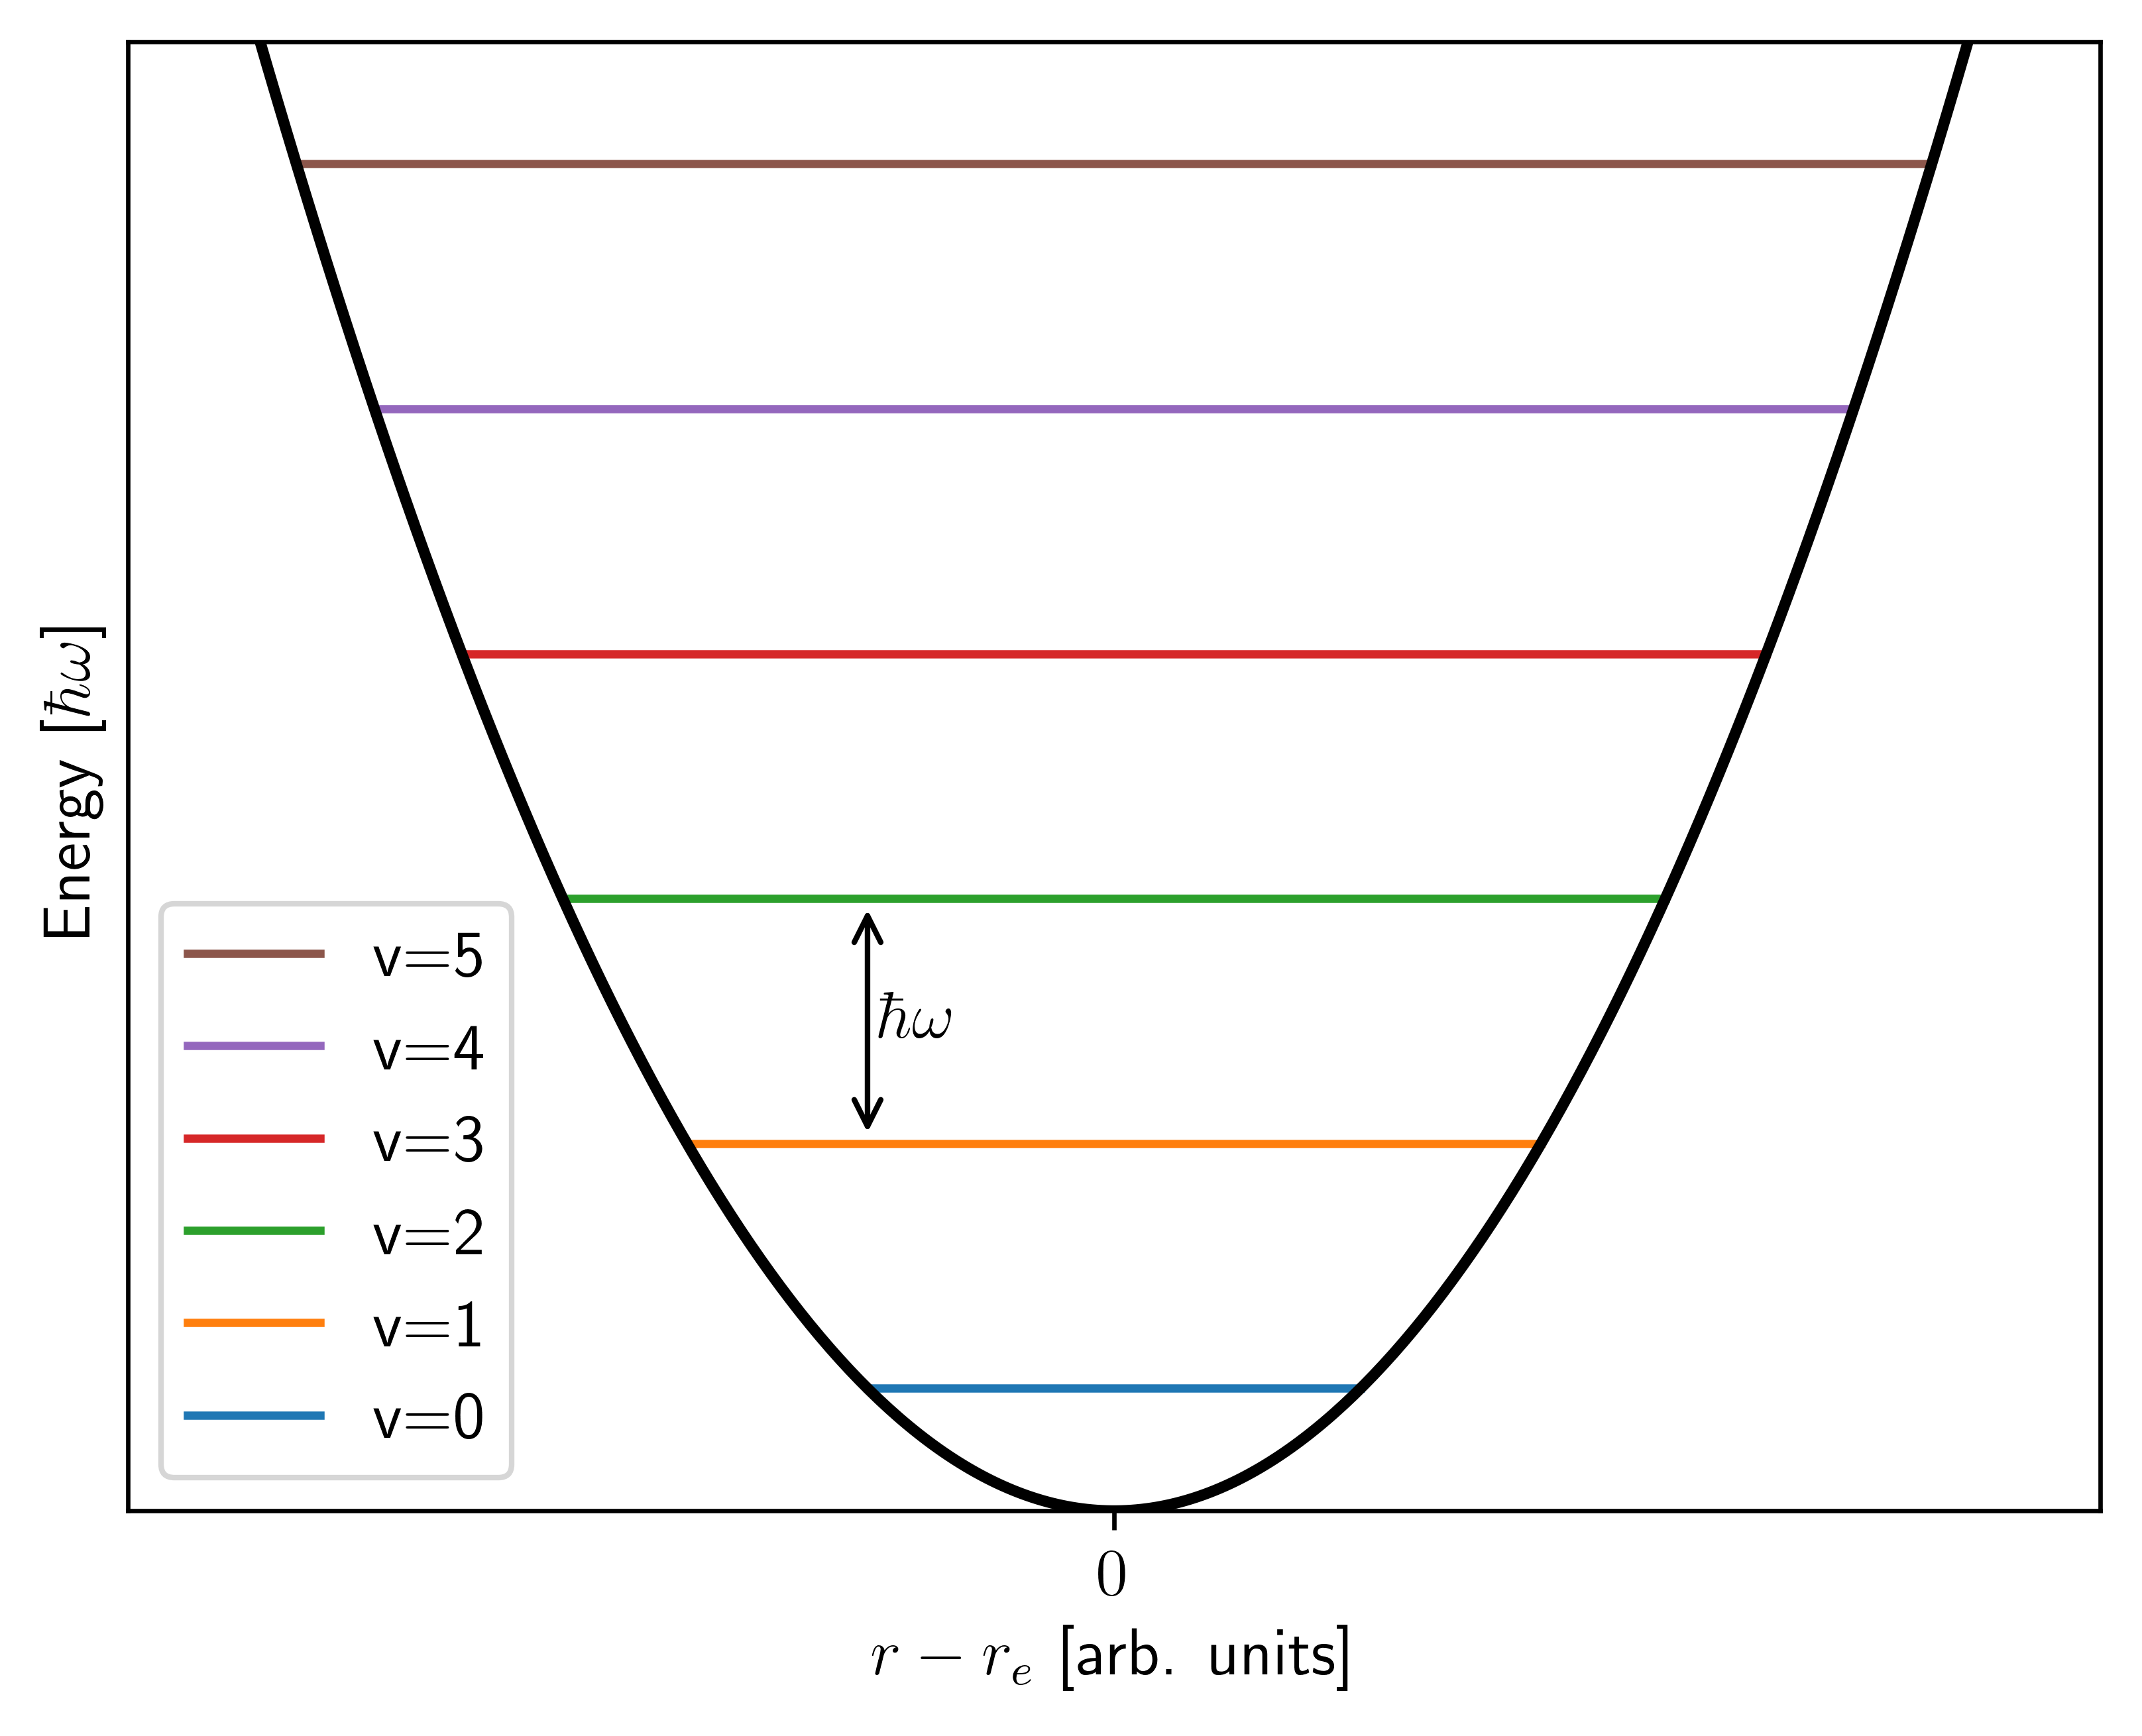
\includegraphics[width=\linewidth]{harmonic_oscillator_energies_gina}
\end{wrapfigure}
So, we can see that our vibrational energies are exactly the same as the ones we derived in Chapter 3! The energy levels will be equally spaced and form a \emph{vibrational ladder} - the picture of the vibrational ladder from Chapter 3 is reproduced here (without the shading of the potential - we're now enthusiastic enough quantum chemists to not need colourful encouragement). Remember that the level spacing is given by $\hbar\omega$, and that we have a \textbf{zero-point energy} of $0.5\hbar\omega$ when $v=0$ - unlike in the rotational case where the particle could have \textbf{zero rotational energy}, when $J=0$. Having understood all this, and being inquisitive scientists, you're probably asking two questions. Firstly, \emph{is the harmonic oscillator model actually any good?} Secondly, \emph{most molecules aren't diatomics, how do we account for more complicated molecules?} These are both excellent questions.    

Fortunately, both of these questions have reasonably straightforward answers. Detailed descriptions are kind of beyond what we're doing here, but I'll explain it enough that you hopefully believe me that we have answers. Considering the first case, the obvious problem with the harmonic oscillator picture is that it \textbf{doesn't allow the bond to break} - as we stretch the bond away from it's equilibrium length, it just gets more and more energy, but won't ever actually break! We can see this in action by looking at a slightly altered version of the figure above - I've now changed the x-axis from just being an arbitrary bond extension $x$, to being the quantity $R-R_e$. $R$ in this case is the actual bond length - i.e how stretched or compressed the bond is. $R_e$ is the \emph{equilibrium bond length} - i.e. how long the bond would be if I didn't stretch or compress it. If $R-R_e > 0$¸ I am \emph{stretching} the bond (because $R>R_e$); whereas if $R-R_e < 0$, I am \emph{compressing} the bond (because $R<R_e$). In reality, as I stretch the bond more and more, eventually it will snap - at this point, the energy stops increasing and will just be constant. In the harmonic oscillator picture, the more I increase $R$, the higher energy the bond has - but it will never actually break.

\begin{wrapfigure}{r}{0.4\textwidth}
\centering
	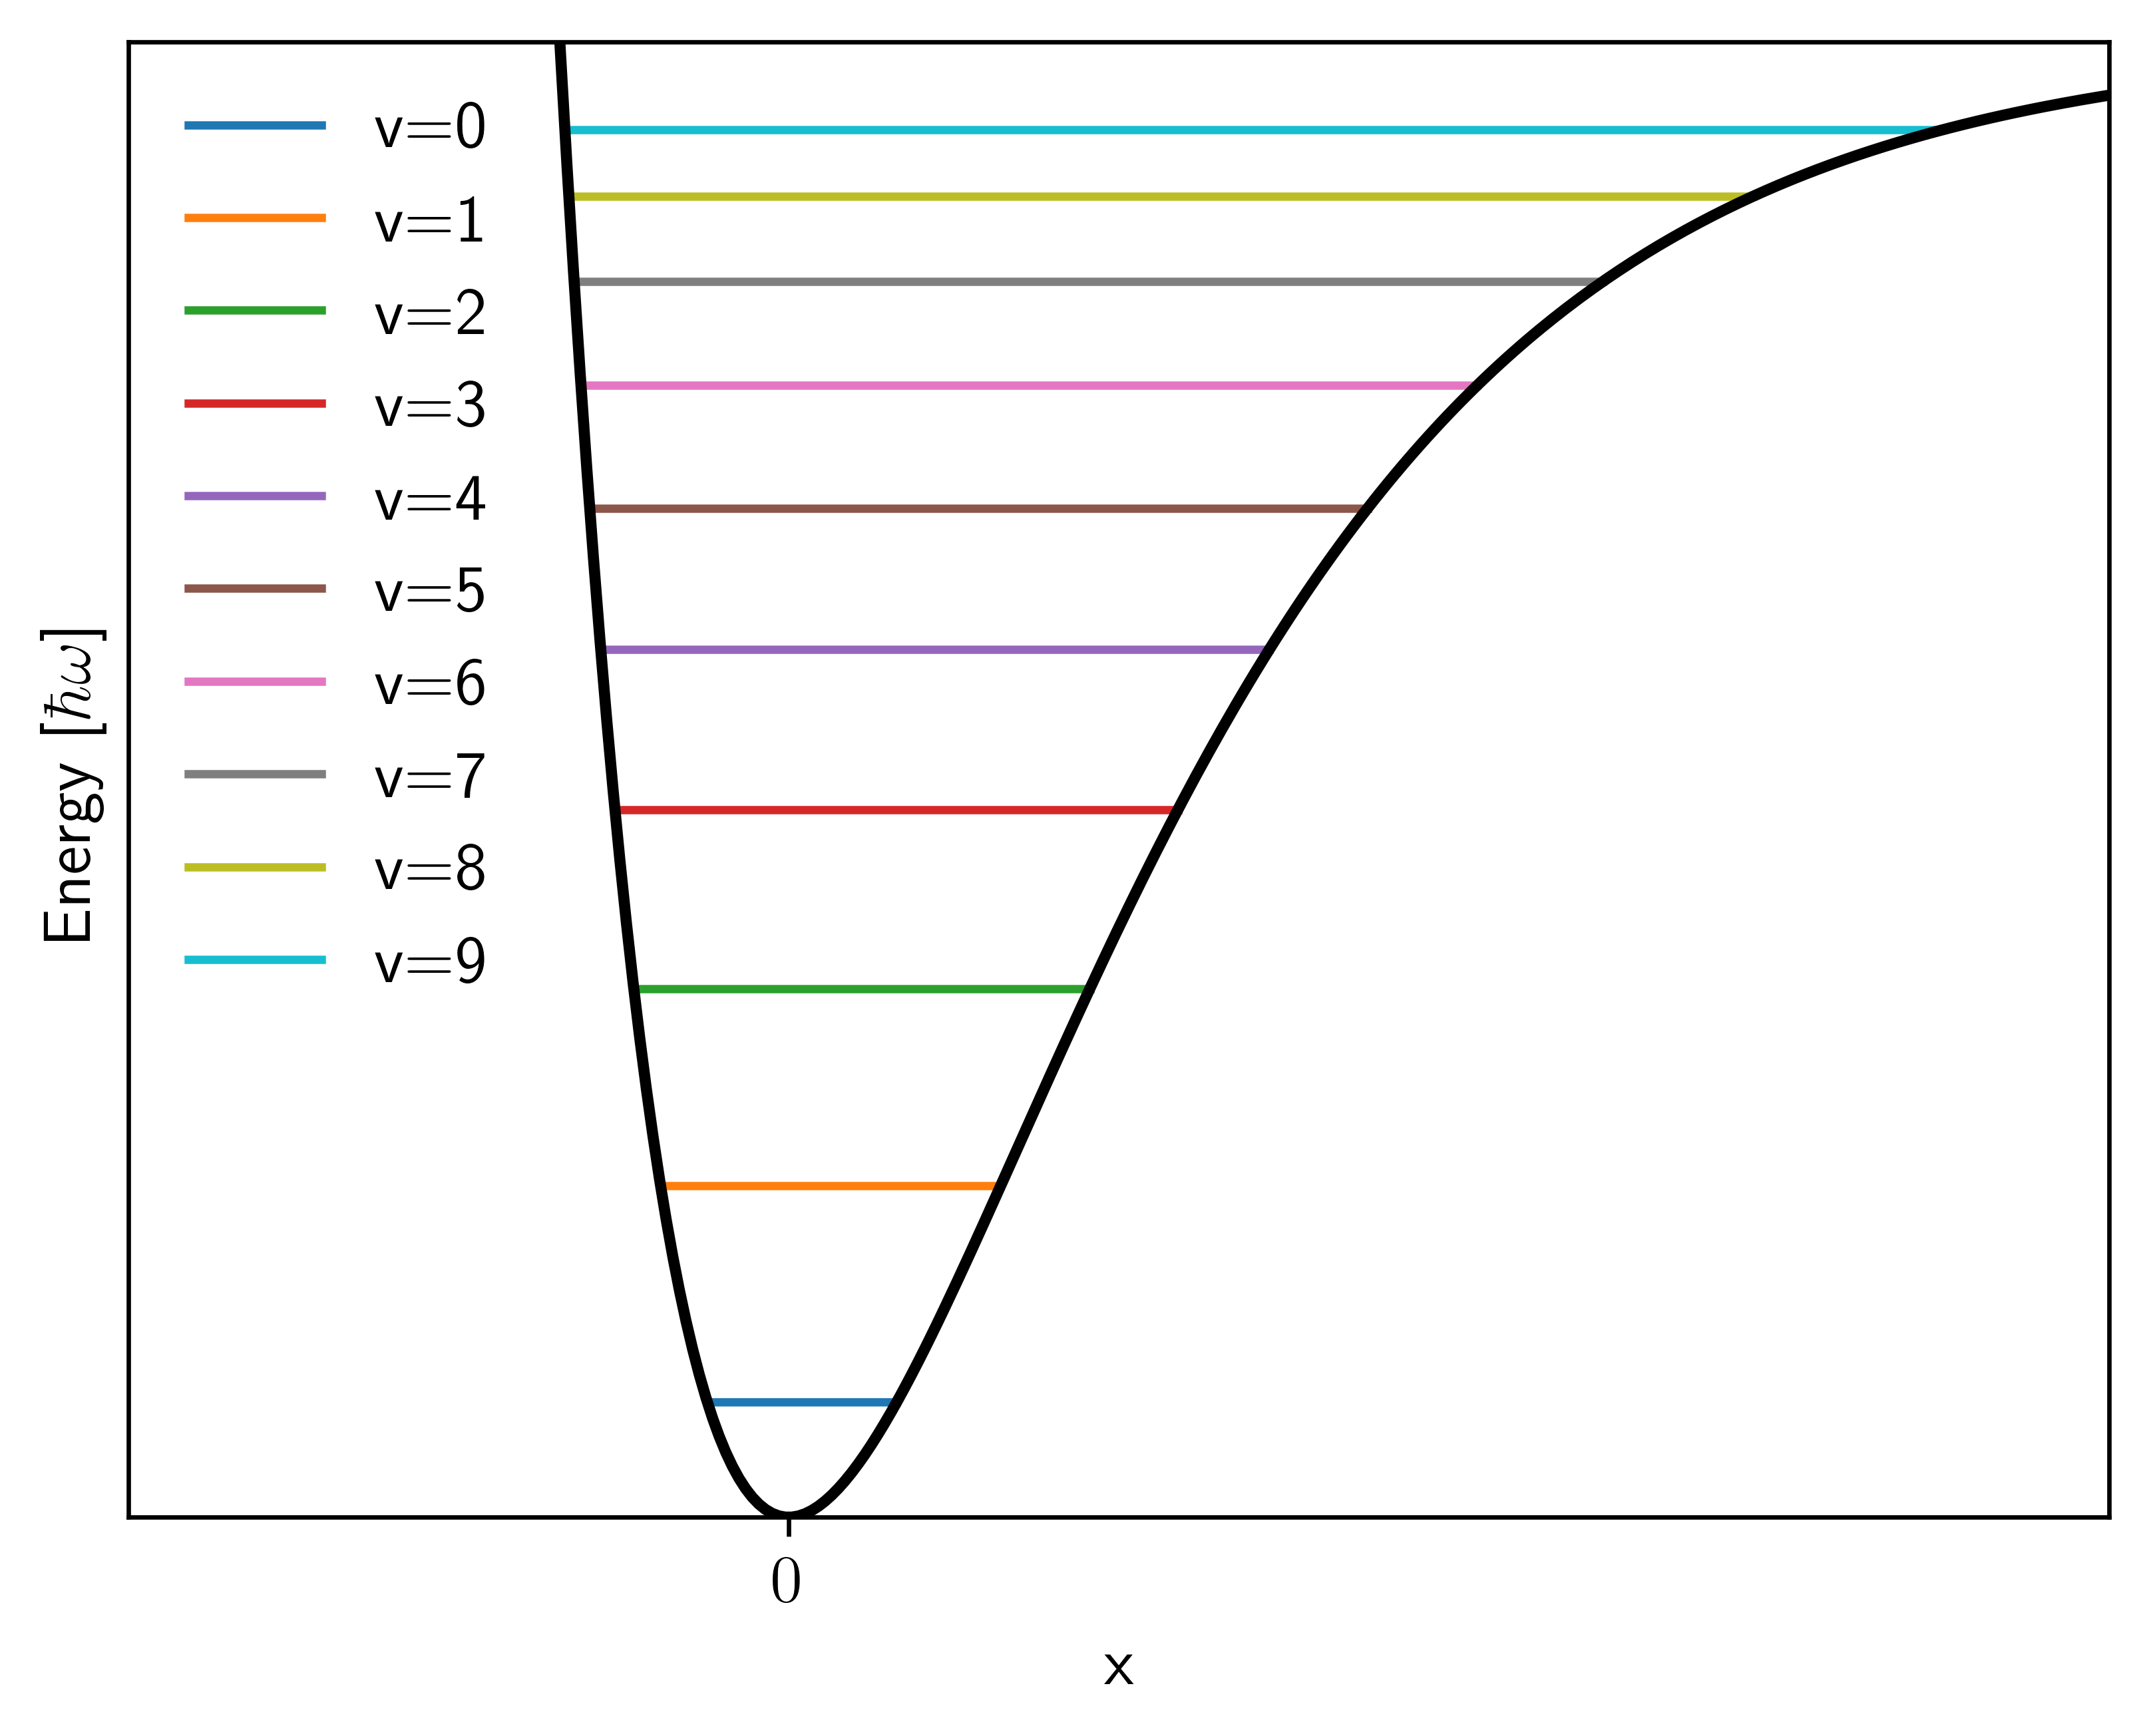
\includegraphics[width=\linewidth]{morse_potential_gina}
\end{wrapfigure}
We get around this by invoking something called \textbf{anharmonicity}, which is most definitely a story for another time. Basically this means that we use a modified potential that \emph{is not harmonic} (i.e. not $V=\frac{1}{2}kx^2$), which allows the bond to break. As a teaser, the energy levels of a classic type of \emph{anharmonic oscillator}, the \textbf{Morse potential}, are shown in the adjacent figure. You can see that the bond is now able to break, the energy is constant for large $R-R_e$ - and the energy spacings are all different too! More on this in a later lecture course.

The second problem, about how we describe non-diatomic molecules, will get an even briefer answer. Essentially, we can break all the molecular vibrations up and find treat \textbf{each vibration as a separate oscillator}. These are called the \textbf{normal modes} of a molecule, and are something you will meet later - especially in the context of molecular symmetry. The method rests on converting the internal molecular coordinates to the so-called \emph{normal coordinates} - if you think that sounds mathematical and tedious, then you are correct! Just be aware that we aren't solely limited to looking at diatomic molecules, and can actually describe real vibrations in complicated molecules (ask Prof. Ellis about his research, this is what he does all day!).

The final thing to consider is the \textbf{vibrational selection rules} - we haven't looked at these yet, and need to find out what vibrational transitions \emph{are actually allowed}. So without further ado...

\subsection{Vibrational Selection Rules}
Having discussed the rotational selection rules in gory detail, this section should be quite easy going - the selection rules are basically the same! Again we have a \textbf{gross} and \textbf{specific} selection rule. Here they are:
\begin{itemize}
	\item Gross Selection Rule: the \emph{dipole moment of the molecule \emph{must} change during the vibration}.
	\item Specific Selection Rule: $\Delta v = \pm 1$.
\end{itemize}
There we have it! So where do these come from? The first one has a similar reasoning behind it to the rotational selection rule. The electric field of the EM radiation can't \emph{grab hold} of the vibration if the dipole moment doesn't change during the vibration. If, as the molecule vibrates, the polarity of the molecule changes - then different bits of the molecule will feel \emph{different amounts of force from the radiation}, and the vibration will be driven harder and harder. Conversely, if the polarity is the same, then every bit of the molecule feels the same force, and the overall result is \emph{no vibration}. If a vibration can be driven by absorption or emission of photons (as described here), it is said to \textbf{infrared active}. 

The second selection rule doesn't really have a nice analogy to help explain it. It actually arises due to the TDM and properties of the \textbf{Hermite Polynomials} that we discussed in Chapter 3. Broadly, when a molecule absorbs some radiation that could excite a vibration, the only states for which the TDM is \textbf{non-zero} are those for which the \textbf{vibrational quantum number} goes up or down by 1. This is due to the symmetry of the \textbf{Hermite Polynomials} - have a look in Atkins' \emph{Molecular Quantum Mechanics} if you're interested! 

It's also worth pointing out (before an organic chemist tries to tell you all I'm talking nonsense), that this specific selection rule \textbf{only applies for harmonic oscillators}. As molecules aren't actually harmonic oscillators, this selection rule can be \textbf{relaxed} somewhat. This means that sometimes in vibrational spectra you'll see things like \textbf{overtones} where $\Delta v = \pm 2$ or $\pm 3$. We can also sometimes \textbf{excite rotations and vibrations simultaneously} - this is called \textbf{rovibrational spectroscopy}, and is something you'll talk about later. An exciting world awaits!

That's more or less it. Let's summarise the vibrational energy levels and selection rules.
\begin{myexampleblock}{\begin{center}Vibrational Spectroscopy\end{center}}
	\begin{center}
		\begin{itemize}
			\item Energy levels (in \si{\per\centi\metre}): $E = (v+\frac{1}{2})\tilde{v}$, where: $\tilde{v} = \frac{1}{2\pi c}\sqrt{\frac{k_f}{\mu}}$
			\item Gross selection rule: dipole moment \textbf{must change during the vibration}.
			\item Specific selection rule: $\Delta v = \pm 1$.
		\end{itemize}
		\end{center}
\end{myexampleblock}

\section{Conclusion}
Well, that's it! This is the end of our short course on introductory quantum mechanics for spectroscopy. I hope you've found it enjoyable and informative, and I'd be over the moon if you agreed with me that this is a beautiful subject worthy of further study! There's a lot of information in this handout, but don't be daunted - look at the \textbf{`course aims'} sheet attached, the idea of this is to tell you what will be considered `examinable', so you know where to target the revision. Some of what I've included in this last section is extra stuff, but I hope you found it interesting nonetheless.

I studied for my PhD in Aarhus, Denmark - the physicists there who graduated from their introductory quantum mechanics course had to make a pledge at the end. The pledge was:
\begin{quote}
	I solemnly swear not to kill Schr{\"o}dingers Cat.
\end{quote}
I think we can agree this would be a fitting end to this course.
















\appendixpage
\appendix
\chapter{Construction of Operators}
Construction of operators is actually quite straightforward. What we do is start from knowing two operators, the \textbf{position} and \textbf{momentum} operators - and then building all the rest from there. The position along $x$ ($\hat{x}$) and momentum along $x$ ($\hat{p_x}$) operators are given by:
\begin{align}
	\hat{x} &= x\times\\
	\hat{p_x} &= -i\hbar \frac{\partial}{\partial x}
\end{align}
So the position operator is just that we do $x$ times whatever comes later, and the momentum operator is that we take the first derivative with respect to $x$, and times it all by $-i\hbar$. These two equations are true provided that we are working in \textbf{position space} or \textbf{the position representation}. Don't worry too much about what this means for now. 

So how do we make operators? It's very simple! We take a classical observable that we want to measure, and find a classical expression for it. If we know the classical expression, then we can easily calculate the quantum mechanical operator just by swapping $x$ for $\hat{x}$ and classical linear momentum along x, $p_x$ for $\hat{p_x}$. For example, if I wanted to find the \textbf{kinetic energy operator}, $\hat{T}$, I would first note that classically:
\begin{equation}
	E_{Kin} = \frac{p_x^2}{2m}
\end{equation}
And therefore that:
\begin{equation}
	\hat{T} = \frac{\hat{p_x}^2}{2m}
\end{equation}
Substituing in the expression for $\hat{p_x}$ we had in the first place, gives me my quantum mechanical kinetic energy operator $\hat{T}$ as:
\begin{equation}
	\hat{T} = -\frac{\hbar^2}{2m}\frac{\partial^2}{\partial x^2}
\end{equation}
It's as easy as that! Similarly, I could find an operator for a \textbf{harmonic potential} (classically: $V = \frac{1}{2}k_fx^2$) as:
\begin{equation}
	\hat{V} = \frac{1}{2}k_f\hat{x}^2 = \frac{1}{2}k_fx^2
\end{equation}
Neat, right? Try and find the operator corresponding to \textbf{angular momentum around the z axis} as a challenge!

\chapter{More Advanced Mathematical Concepts in QM}
\section{Dirac Bra-ket Notation}
It turns out we end up doing a lot of integrals when we start to get into quantum mechanics. This can be a bit of a pain to keep writing out, so the English physicist and all-round legend Paul Dirac developed his \textbf{bra-ket notation} to make it all easier. In bra-ket notation, an integral can be written as follows:
\begin{equation}
	\int \phi^* \hat{O} \psi \mathrm{d}\tau = \bra{\phi}\hat{O}\ket{\psi}
\end{equation}
Where the $\bra{\phi}$ bit is called a `bra', and the $\ket{\psi}$ bit is called a `ket'. Strictly, the $\ket{\psi}$ represents the \textbf{quantum mechanical state} described by the wavefunction $\psi$. If I had a bra $\bra{\psi}$, that would represent the \textbf{complex conjugate} of the wavefunction $\psi$. Bra-ket notation makes everything a lot neater, for instance I can now write my Schr{\"o}dinger Equation as:
\begin{equation}
	\hat{H}\ket{\psi} = E\ket{\psi}
\end{equation}
And I can write my normalisation integrals as simply:
\begin{equation}
	\bra{\psi}\ket{\psi} = 1
\end{equation}
So you can see how it makes things a bit neater and cleaner! If you get really into this, you'll start to learn about how the bras and kets can represent \textbf{matrix elements}, which is a key concept for more advanced quantum mechanics. Some books also like to use this notation without ever explaining it and assuming that everyone knows what it is - so this should help you if you come across one of those!
\section{Hermitian Operators}
This is a really critical concept once you start to get more into the maths behind quantum mechanics. Hermitian operators are named after Charles Hermite of Hermite Polynomial fame. Using our new bra-ket notation, an operator $\hat{O}$ is defined as \textbf{Hermitian} if:
\begin{equation}
	\bra{\phi}\hat{O}\ket{\psi} = \bra{\psi}\hat{O}\ket{\phi}^*
\end{equation}
So the operator $\hat{O}$ is \textbf{Hermitian} if we can swap the states it's operating on and take a complex conjugate, and obtain the same result. Don't worry much about this, but hermitian operators have two very important qualities for quantum mechanics:
\begin{enumerate}
	\item The eigenvalues of a Hermitian operator are \textbf{necessarily real}.
	\item Eigenfunctions corresponding to different eigenvalues of a Hermitian operator are \textbf{necessarily orthogonal}
\end{enumerate}
These are important, because physical observables like energy have to be \textbf{real} - so the operators that give them must be \textbf{Hermitian}. The second means that eigenfunctions of different energy states can't overlap - which would be important if we were getting more into this. Consider this to be a titillating teaser of the importance.



\chapter{Classification of Molecular Rotors}
However, this expression is a \textbf{bit sneaky}. The problem we are going to have is that now we are a molecule rotating in 3D, we could quite plausibly have \textbf{different moments of inertia around different rotation axes}, and therefore we would have \textbf{different angular momenta around different rotation axes}. So strictly, we need to treat the rotation about each axis \textbf{separately}. This means that actually we can write:
\begin{equation}
	E_{\text{Rot.}} = \frac{J_a^2}{2I_a} + \frac{J_b^2}{2I_b} + \frac{J_c^2}{2I_c}
\end{equation}
What we have done here is call each of our three possible rotation axes $a, b$, and $c$. Then each axis has it's own angular momentum $J$ and own moment of inertia $I$. Comparing the two equations above we can see that our the square of our total angular momentum, $J^2$ is equal to the sum of the square of the components, that is:
\begin{equation}
	J^2 = J_a^2 + J_b^2 + J_c^2
\end{equation}
\chapter{Transition Dipole Moments}

\end{document}

